\documentclass{beamer}
\usefonttheme{serif} % default family is serif

\usepackage{beamerthemesplit}
\usetheme{CambridgeUS}
\usecolortheme{beaver}
\usepackage{subfigure}
\usepackage{multirow}
\usepackage{epsfig}
\usepackage[all,knot]{xy}
\xyoption{arc}
\usepackage{url}
\usepackage{multimedia}
\usepackage{hyperref}
\usepackage{setspace}
\usepackage{caption}
\usepackage{fixltx2e}
\usepackage[T1]{fontenc}
\usepackage[utf8]{inputenc}
\usepackage{amsmath}
\usepackage{txfonts}
\usepackage{amsfonts}
\usepackage[mathscr]{euscript}
\usepackage{amsfonts}
\usepackage{dsfont}

\usepackage[export]{adjustbox}% http://ctan.org/pkg/adjustbox
\usepackage{colortbl}
  \newcommand{\myrowcolour}{\rowcolor[gray]{0.925}}
\usepackage{booktabs}
\usepackage{siunitx}
\usepackage{tabularx}
\usepackage{tabulary}
\usepackage{multirow}

\usepackage{tikz}

\usepackage{morewrites}%Always room for a new write stream, permet de creer de nouveau glossaire avec la commande newglossary sinon ca ne marche pas
\usepackage{libertine} % to make \bfseries and \scshape work together

\usepackage{makecell}

\let\olditem\item
\renewcommand{\item}{\setlength{\itemsep}{\fill}\olditem}

\renewcommand\theadalign{cb}
%\renewcommand\theadfont{\bfseries}
\renewcommand\theadgape{\Gape[4pt]}
\renewcommand\cellgape{\Gape[4pt]}

\usepackage[skins,theorems]{tcolorbox}
\tcbset{highlight math style={enhanced, colframe=red,colback=white,arc=0pt,boxrule=1pt}}

\usepackage[acronyms,symbols,nonumberlist,sort=standard]{glossaries}

\setbeamertemplate{caption}{\raggedright\insertcaption\par}
\setbeamerfont{caption}{size=\scriptsize}
\setbeamertemplate{itemize items}[triangle]


\title[LML, CRIStAL, Univ. Lille]{ \bfseries \scshape \large Reconstruction of high-resolution velocity fields in turbulent flows from low-resolution measurements}
\author[L.V.Nguyen]{\bfseries \scshape \footnotesize Linh Van NGUYEN {\vskip -1em}}
\institute[]{\inst{} \scshape \scriptsize LML FRE 3723, CRIStAL-CNRS UMR 9189 \and \vskip-1em \inst{} \scshape  \scriptsize Universit\'e de Lille, 59655 Villeneuve d'Ascq}
\date[\today]{\scshape \tiny \today \\ {\vskip 1em}
{\scriptsize \centering
\begin{tabular}[t]{@{}l@{\hspace{5pt}}p{.28\textwidth}@{}}
Jury members: & Dr. Etienne M\'EMIN \\
& Pr. Olivier MICHEL\\
& Pr. Danaila LUMINITA\\
& Pr. Nicolas DOBIGEON
\end{tabular}%
\begin{tabular}[t]{@{}l@{\hspace{5pt}}p{.28\textwidth}@{}}
Supervisors: & Dr. Jean-Philippe LAVAL \\ 
& Dr. Pierre CHAINAIS
\end{tabular}
}
{\vskip 2em}
}

\titlegraphic{
	
\includegraphics[height=1cm]{./figures/logos/LML.png}
	\hspace*{0.15cm}~%
	
\includegraphics[height=1cm]{./figures/logos/crystal.png}
	\hspace*{0.15cm}~%
	
\includegraphics[height=1cm]{./figures/logos/lille1.png}
	\hspace*{0.15cm}~%
	
\includegraphics[height=1cm]{./figures/logos/ECLille.png}
	\hspace*{0.15cm}~%
	
\includegraphics[height=1cm]{./figures/logos/CNRS.png}
	\hspace*{0.15cm}~%
	
\includegraphics[height=0.75cm]{./figures/logos/haut_france.jpg}	
}

\newcommand{\backupbegin}{
   \newcounter{finalframe}
   \setcounter{finalframe}{\value{framenumber}}
}
\newcommand{\backupend}{
   \setcounter{framenumber}{\value{finalframe}}
}

%\AtBeginSection[]{
%  \begin{frame}
%  \vfill
%  \centering
%  \begin{beamercolorbox}[sep=8pt,center,shadow=true,rounded=true]{title}
%    \usebeamerfont{title}\insertsectionhead\par%
%  \end{beamercolorbox}
%  \vfill
%  \end{frame}
%}

\everymath{\displaystyle}
\DeclareMathOperator*{\argmax}{\arg\!\max}
\DeclareMathOperator*{\argmin}{\arg\!\min}

\DeclareMathOperator{\sign}{sign}
\DeclareMathOperator{\prox}{prox}

\newcommand{\mybold}[1]{\ensuremath{\operatorname{\boldsymbol{#1}}}}
\newcommand{\mydef}{\triangleq}
\newcommand{\mytrans}{\intercal}
\newcommand{\mypseudo}{\dagger}
\newcommand{\myhat}[1]{\ensuremath{\operatorname{\hat{#1}}}}
\newcommand{\myexp}[1]{\ensuremath{\operatorname{\exp{ \left(#1\right)}}}}
\newcommand{\mysign}[1]{\ensuremath{\operatorname{\sign{\left(#1\right)}}}}
\newcommand{\mydot}{\cdot} 

\newcommand{\R}{{\rm I\!R}}
\newcommand{\subjectto}{\:\:\:\:\:\: s.t. \:\:\:\:\:\:}
\newcommand{\Df}{D_f}
\newcommand{\dimsh}{P}
\newcommand{\dimsl}{Q}
\newcommand{\dimth}{N}
\newcommand{\dimtl}{M}
\newcommand{\dimpsh}{p}
\newcommand{\dimpsl}{q}
\newcommand{\dimpth}{n}
\newcommand{\dimptl}{m}
\newcommand{\dimdict}{K}
\newcommand{\dimtrunc}{L}

\newcommand{\dimpacc}{r} % accumulative patch size
\newcommand{\dimpsr}{s} % searching region size
\newcommand{\nlmfilparam}{\sigma} % accumulative patch size \tau

\newcommand{\neighbor}{\mathcal{N}}
\newcommand{\mymapto}{\longmapsto}
\newcommand{\mymapfrom}{\mathrel{\reflectbox{\ensuremath{\mymapto}}}}

\newcommand{\z}{\mybold{z}}
\newcommand{\y}{\mybold{y}}
\newcommand{\x}{\mybold{x}}
\newcommand{\Z}{\mathbf{Z}}
\newcommand{\Y}{\mathbf{Y}}
\newcommand{\X}{\mathbf{X}}
\newcommand{\B}{\mathbf{B}}
\newcommand{\I}{\mathbf{I}}
\newcommand{\Diag}{\mathbf{D}}
\newcommand{\Umat}{\mathbf{U}}
\newcommand{\Vmat}{\mathbf{V}}

\newcommand{\LR}{\y}
\newcommand{\HR}{\z}
\newcommand{\LF}{\z_{lf}}
\newcommand{\HF}{\z_{hf}}
\newcommand{\HFest}{\hat{\z }_{hf}}

\newcommand{\h}{\mybold{h}}
\newcommand{\n}{\mybold{n}}
\newcommand{\boundHF}{\mybold{b}}

\newcommand{\knot}{{\circ}}
\newcommand{\ext}{{e}} % denote the generalization data for prediction

\newcommand{\Interp}{\varmathbb{I}}
\newcommand{\Sub}{\varmathbb{S}}
\newcommand{\LPF}{\varmathbb{L}}

\newcommand{\distr}{\mathscr{N}} 
\newcommand{\loss}{\mathcal{L}}

\newcommand{\normtwo}[1]{\ensuremath{\operatorname{\Arrowvert  \mathit{#1} \Arrowvert^2_2 }}}
\newcommand{\Mdist}[2]{\ensuremath{\operatorname{\Arrowvert \mathit{#1} \Arrowvert^2_{\mathit{#2}} }}}
\newcommand{\normone}[1]{\ensuremath{\operatorname{\Arrowvert \mathit{#1} \Arrowvert_1 }}}
\newcommand{\normzero}[1]{\ensuremath{\operatorname{\Arrowvert  \mathit{#1} \Arrowvert_0 }}}
\newcommand{\normp}[1]{\ensuremath{\operatorname{\Arrowvert  \mathit{#1} \Arrowvert_p }}}

\newcommand{\detmat}[1]{\ensuremath{\operatorname{\left|  \mathit{#1} \right| }}}
\newcommand{\cov}[1]{\ensuremath{\operatorname{cov \left\lbrace  \mathit{#1} \right\rbrace }}}
\newcommand{\E}[1]{\ensuremath{\operatorname{E \left[  \mathit{#1} \right] }}}
\newcommand{\tr}[1]{\ensuremath{\operatorname{tr \left\lbrace  \mathit{#1} \right\rbrace }}}
\newcommand{\Conv}{\mathop{\scalebox{1.5}{\raisebox{-0.2ex}{$\ast$}}}}

\newcommand{\pinv}[1]{\ensuremath{\operatorname{  \mathit{#1} ^\dagger}}}
%\newcommand{\featmap}[1]{\ensuremath{\operatorname{  \mathcal{F} \left(#1\right)}}}
\newcommand{\featmap}[1]{\ensuremath{\operatorname{ \varphi \left(\mathit{#1}\right)}}}

%\newcommand{\dict}{\mathds{D}}
%\newcommand{\dictco}{\mathds{A}}
\newcommand{\dict}{\mathbf{D}}
\newcommand{\dictco}{\mathbf{A}}
\newcommand{\adict}{\boldsymbol{d}}
\newcommand{\adictco}{\boldsymbol{a}}

\newcommand{\patchlow}[1]{\ensuremath{\operatorname{\mathit{\mybold{p}_{\ell}^{#1}}}}}
\newcommand{\patchhigh}[1]{\ensuremath{\operatorname{\mathit{\mybold{p}_h^{#1}}}}}
\newcommand{\dictlow}{\dict_\ell}
\newcommand{\dicthigh}{\dict_h}
\newcommand{\adictcolow}[1]{\ensuremath{\operatorname{\boldsymbol{a}_\ell^{\mathit{#1}}}}}
\newcommand{\adictcohigh}[1]{\ensuremath{\operatorname{\mathit{\boldsymbol{a}_h^{#1}}}}}
\newcommand{\adictlow}[1]{\ensuremath{\operatorname{\boldsymbol{d}_\ell^{\mathit{#1}}}}}
\newcommand{\adicthigh}[1]{\ensuremath{\operatorname{\mathit{\boldsymbol{d}_h^{#1}}}}}

\newcommand{\extractlow}[1]{\ensuremath{\operatorname{\mathcal{R}_{\ell}^{\mathit{#1}}}}}
\newcommand{\extracthigh}[1]{\ensuremath{\operatorname{\mathit{\mathcal{R}_h^{#1}}}}}
\newcommand{\extract}[1]{\ensuremath{\operatorname{\mathcal{R}^{\mathit{#1}}}}}


\newcommand{\mytrace}[1]{\ensuremath{\operatorname{\text{Tr} \left( #1 \right)}}}


\begin{document}
\begin{frame}[noframenumbering]
\titlepage
\end{frame}

% % % % % % % % % % % % % % % % % % % % % % % % % % % % % % % % % % % % % % % % % % % % % %
% % % % % % % % % % % % % % % % % % % % % % % % % % % % % % % % % % % % % % % % % % % % % %
% % % % % % % % % % % % % % % % % % % % % % % % % % % % % % % % % % % % % % % % % % % % % % 

\section[Outline]{}
\frame{\tableofcontents}


% % % % % % % % % % % % % % % % % % % % % % % % % % % % % % % % % % % % % % % % % % % % % %
% % % % % % % % % % % % % % % % % % % % % % % % % % % % % % % % % % % % % % % % % % % % % %
% % % % % % % % % % % % % % % % % % % % % % % % % % % % % % % % % % % % % % % % % % % % % % 

\section[Problem definition]{Problem definition}
\subsection[Context of the present work]{Context of the present work}
\begin{frame}
\frametitle{Turbulence is multiscale}
	\begin{itemize}
		\item \textbf{\color{red}Large scales} carry most of kinetic energy, responsible for flow dynamics and transportation of matter
		\item \textbf{\color{red}Small scales} are more related to dissipation properties; more universal
	\end{itemize}
	\begin{overprint}
	\onslide<1>	
	\begin{figure}
		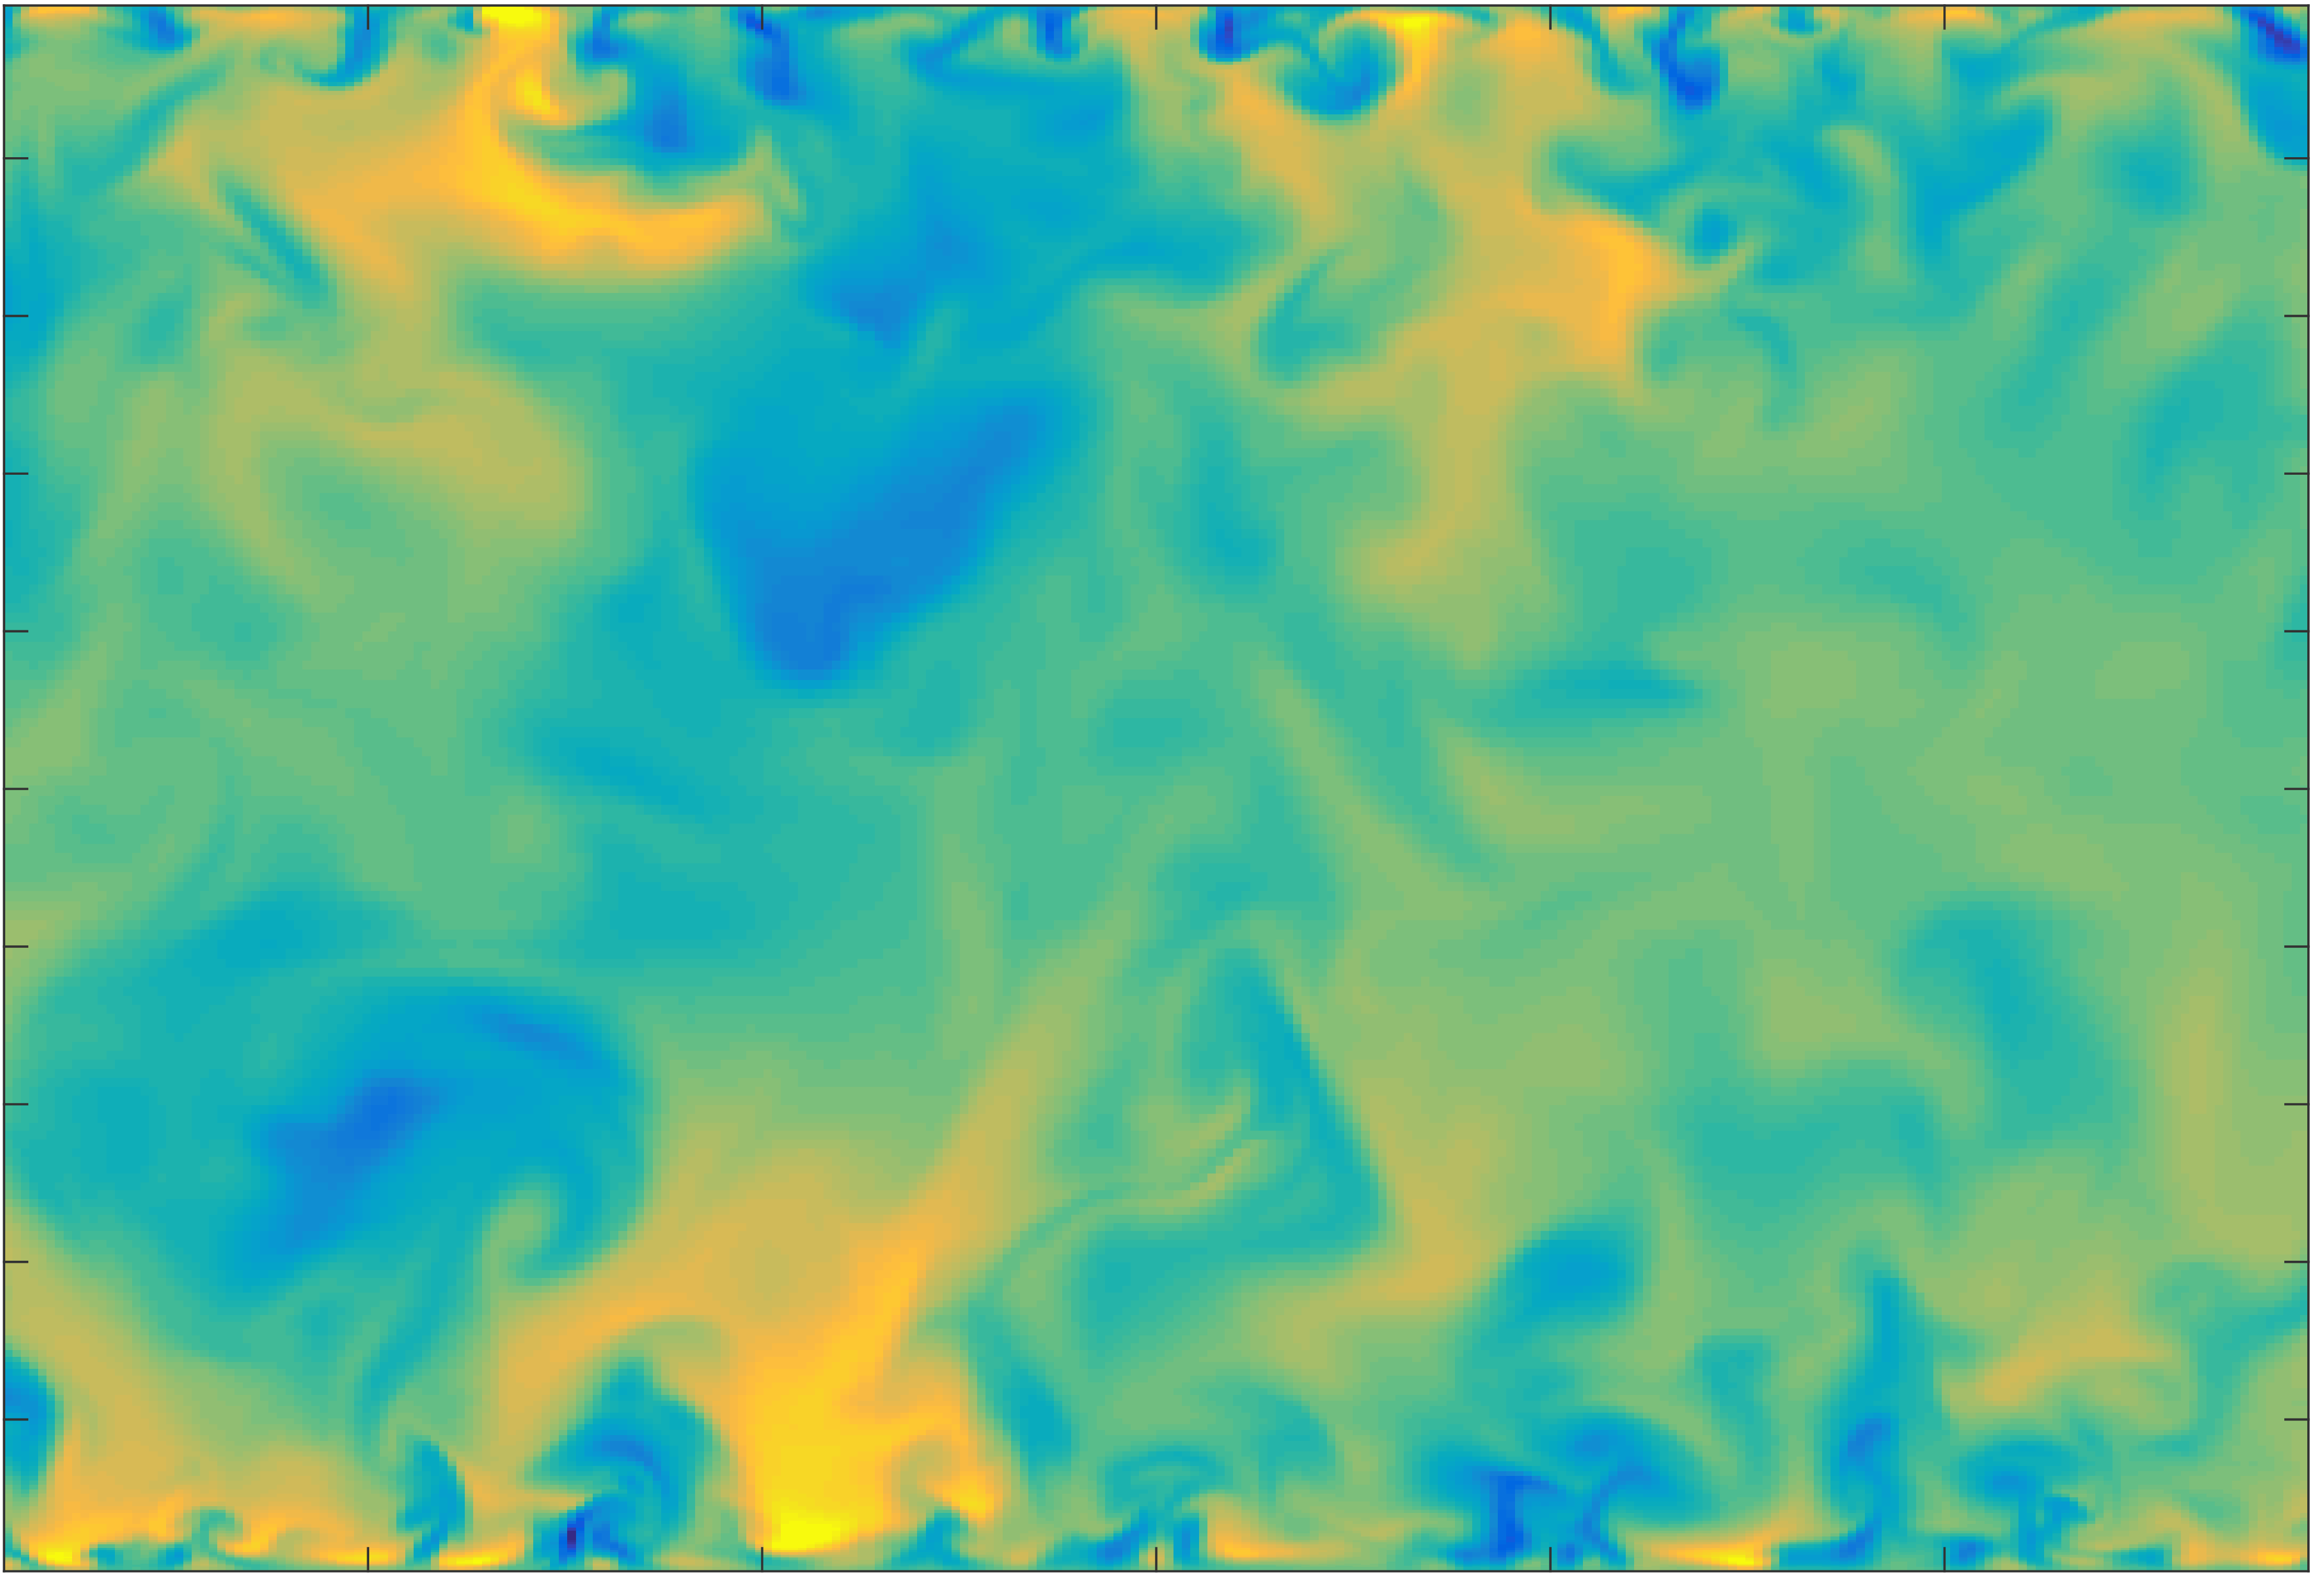
\includegraphics[height=3.75cm,valign=t]{./figures/turbulence/Uorg.png}
		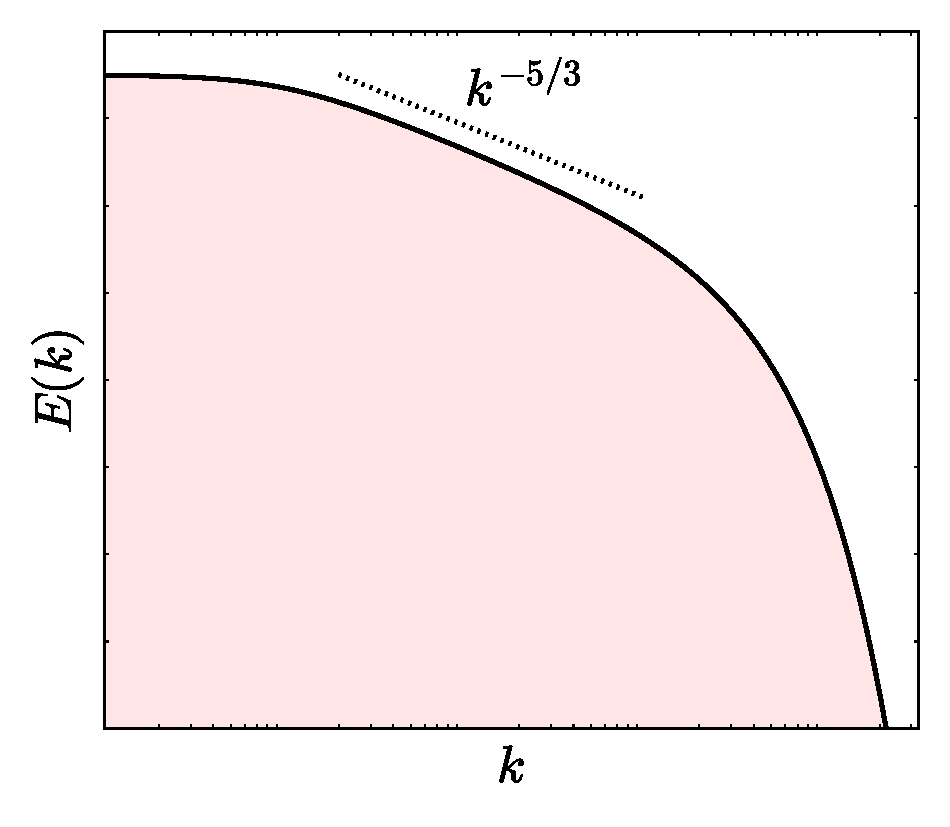
\includegraphics[height=4.1cm,valign=t]{./figures/turbulence/turbulence_spectra_allranges.eps}
		\caption*{Sample streamwise velocity field of a channel flow ($ Re_\tau = 550$) and a synthesized spectrum (all scales)}
	\end{figure}	
	\onslide<2>	
	\begin{figure}
		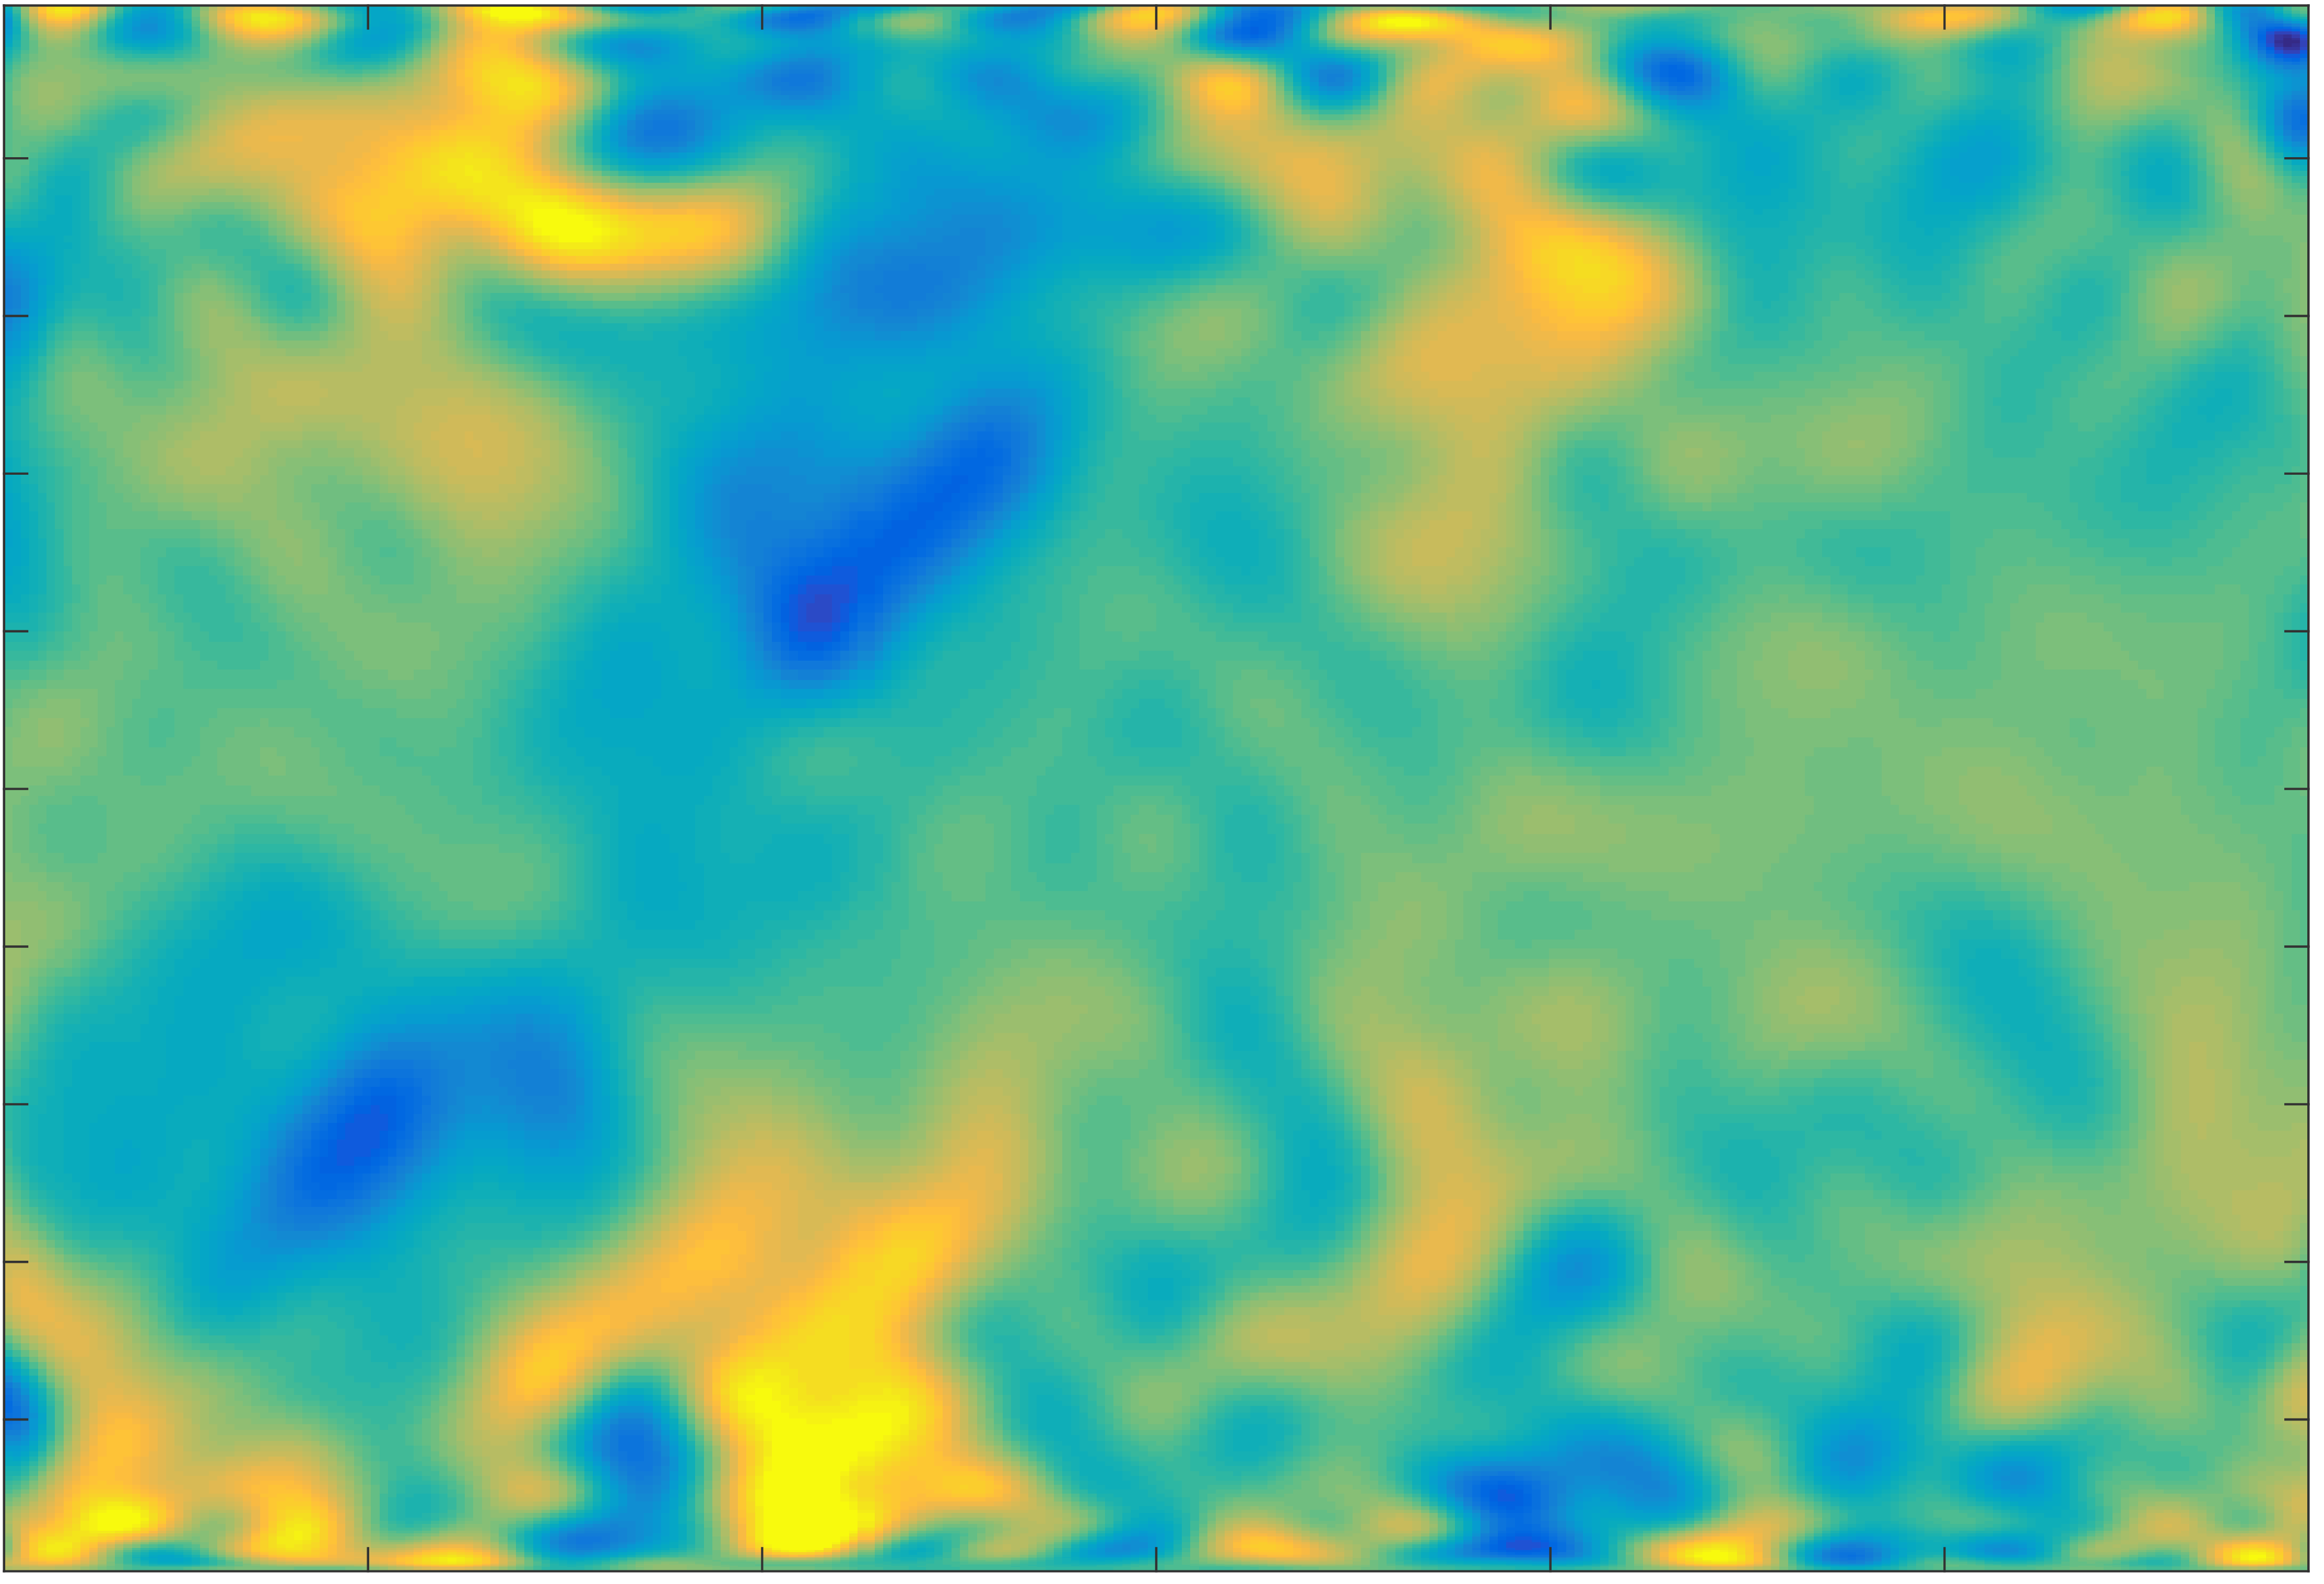
\includegraphics[height=3.75cm,valign=t]{./figures/turbulence/Ularge.png}
		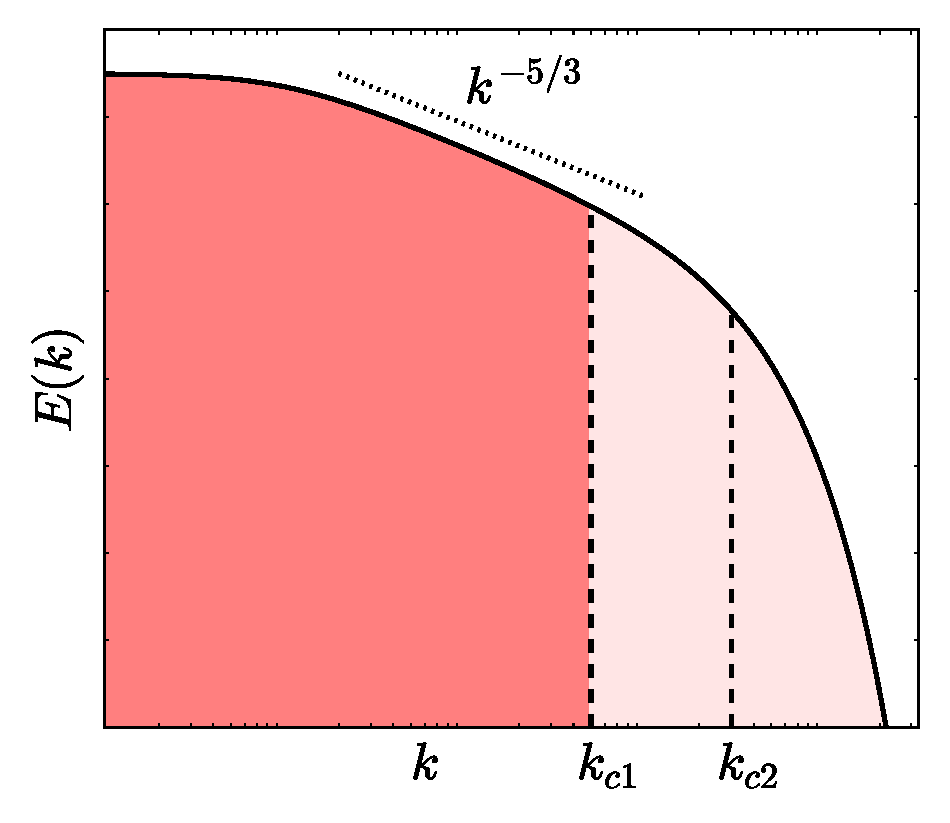
\includegraphics[height=4.1cm,valign=t]{./figures/turbulence/turbulence_spectra_variousranges1.eps}
		\caption*{Sample streamwise velocity field of a channel flow ($ Re_\tau = 550$) and a synthesized spectrum (large scales)}
	\end{figure}
	\onslide<3>	
	\begin{figure}
		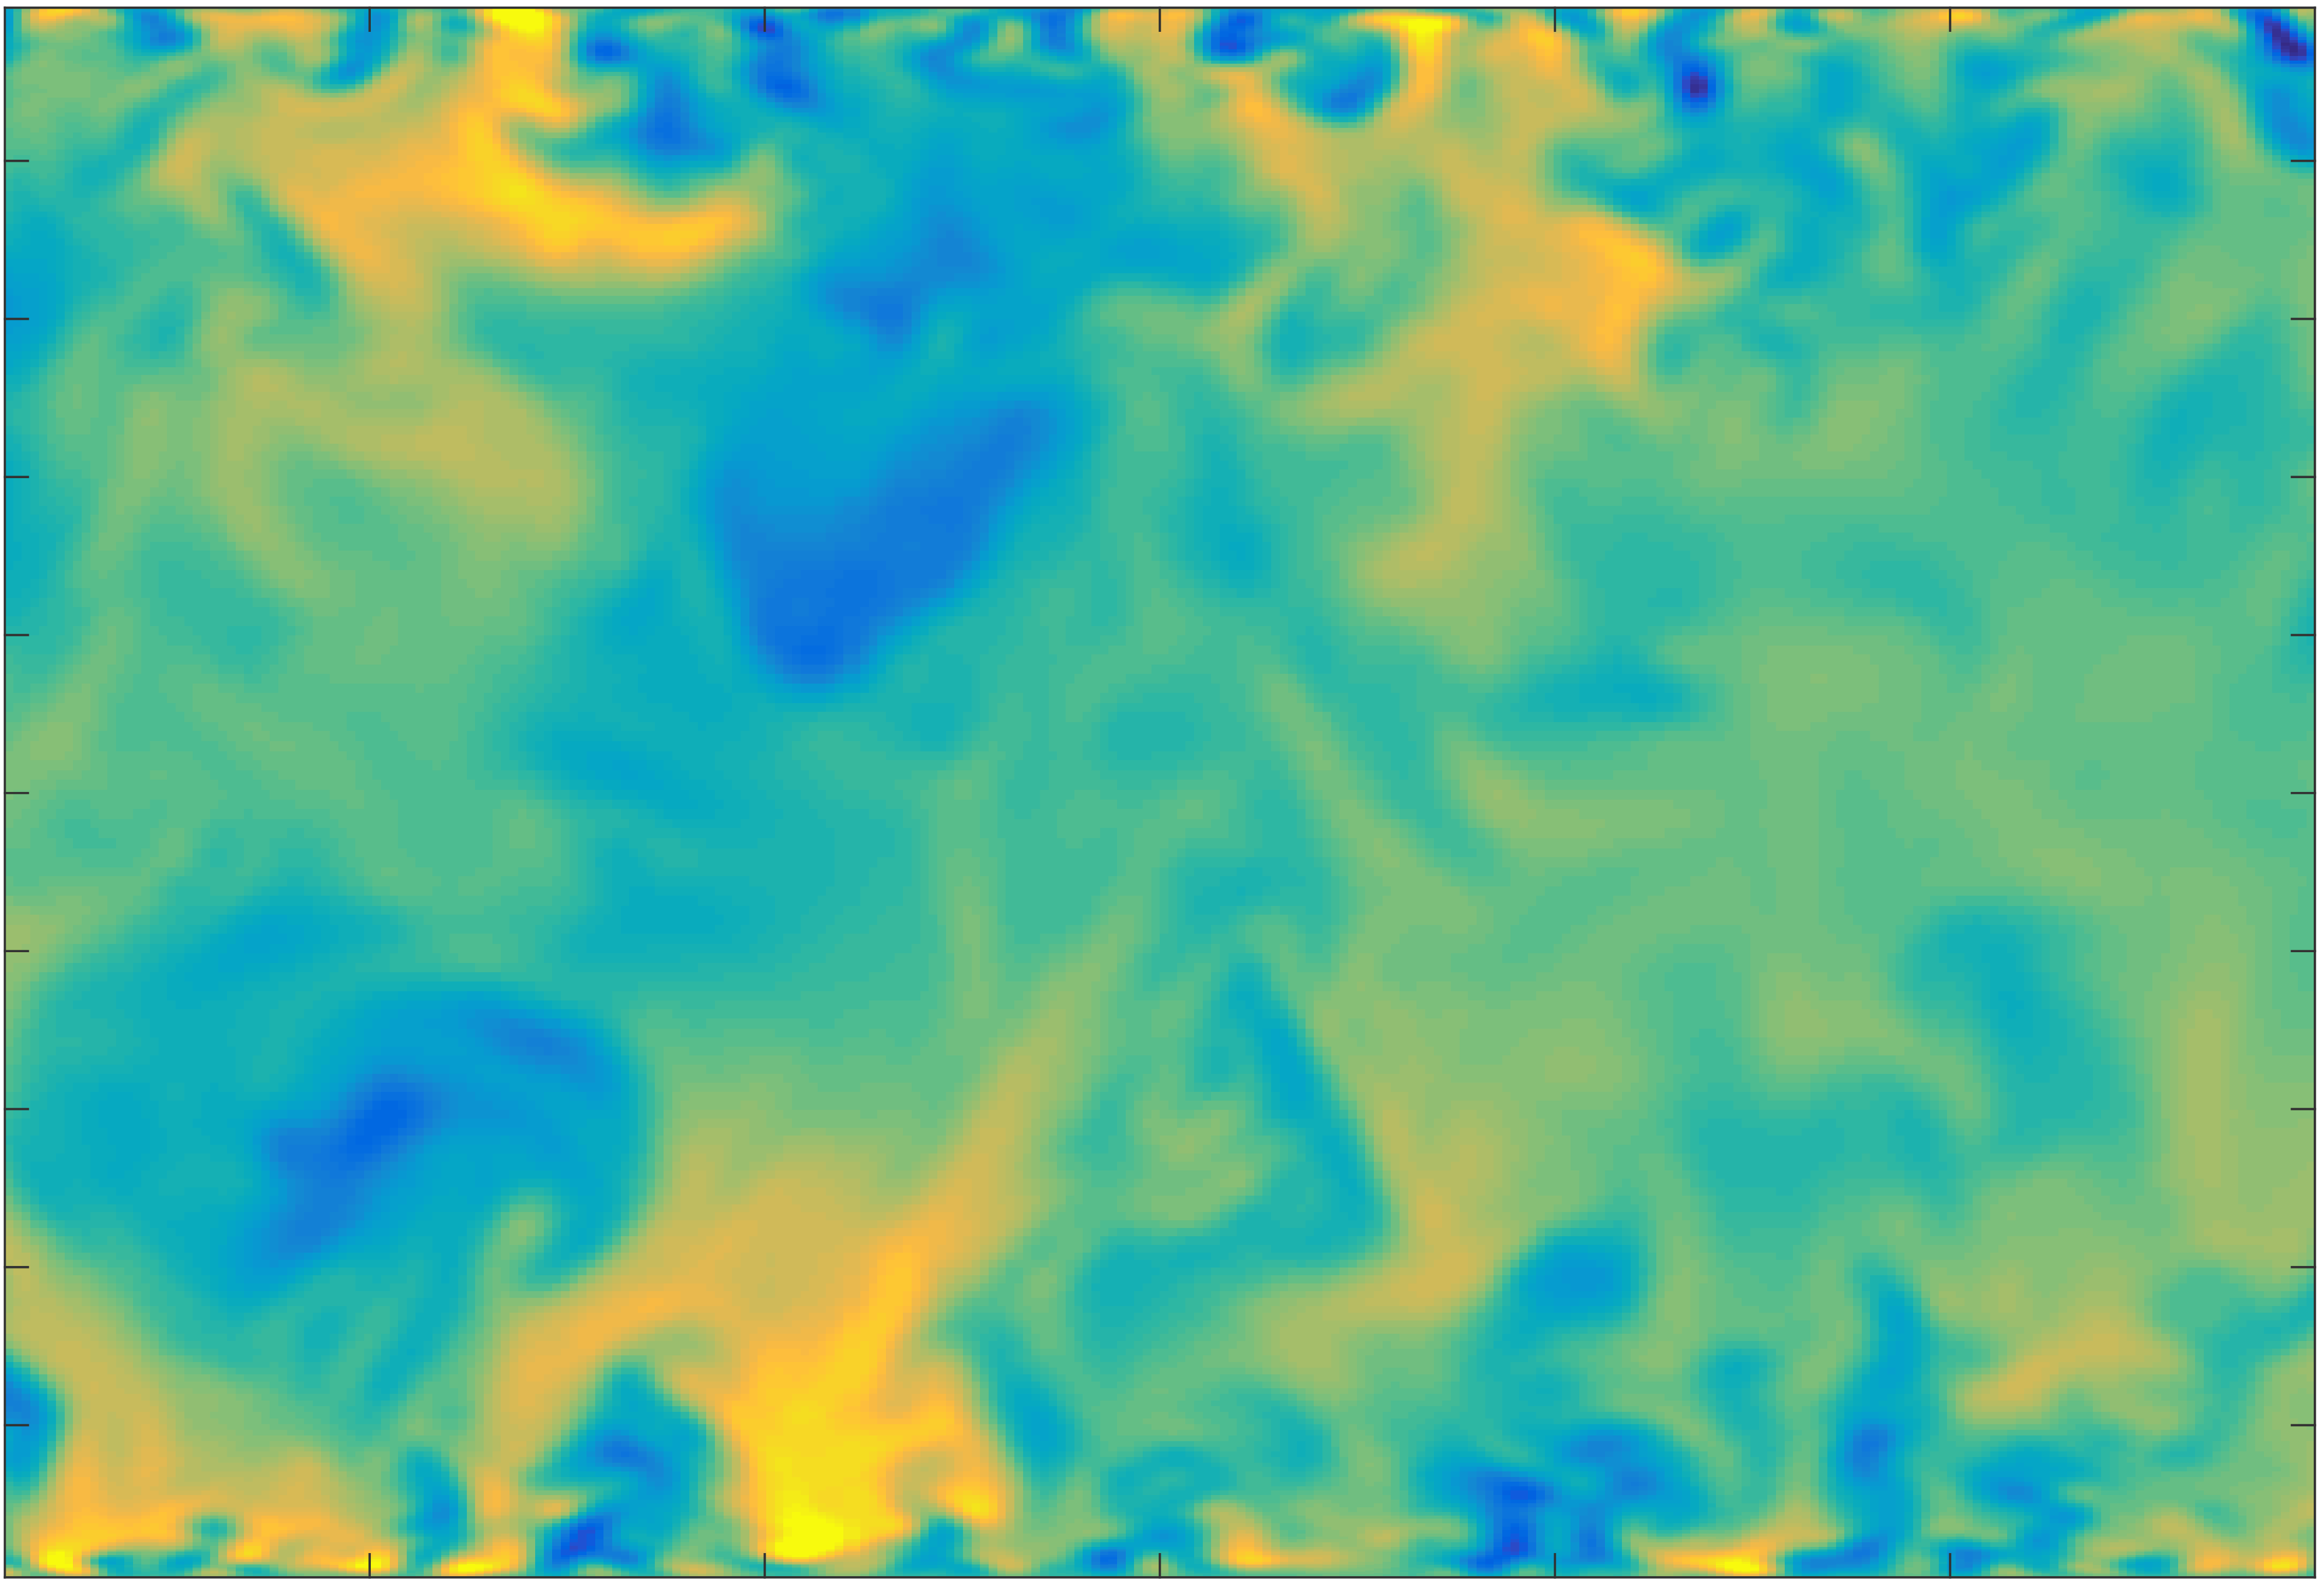
\includegraphics[height=3.75cm,valign=t]{./figures/turbulence/Ulargemid.png}
		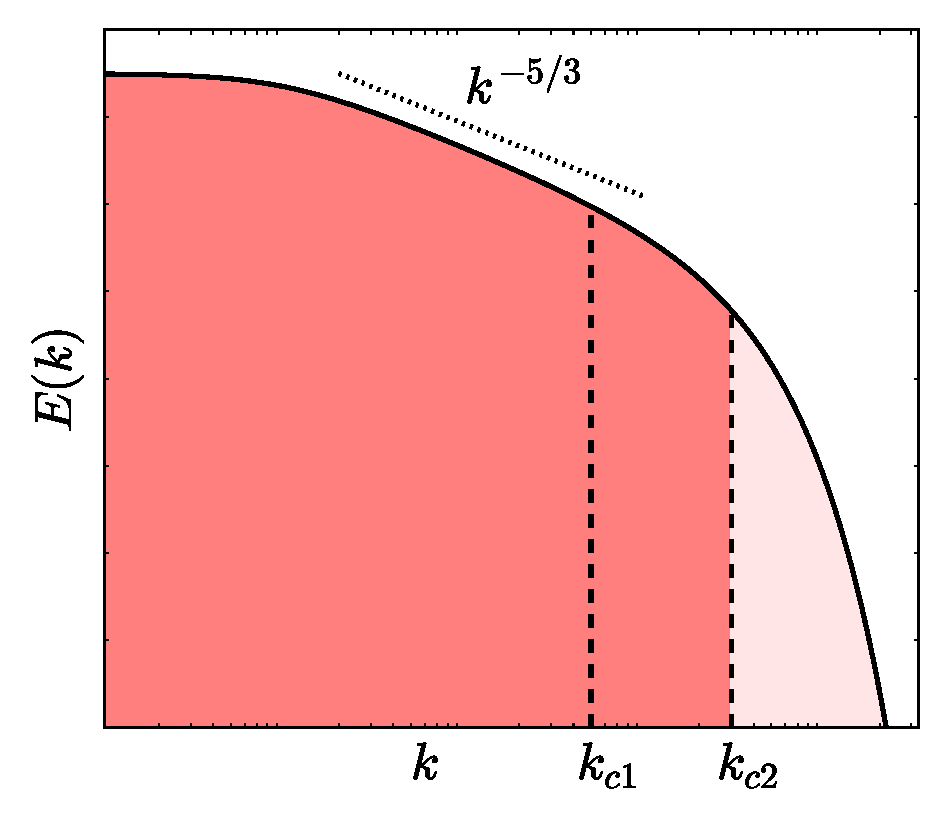
\includegraphics[height=4.1cm,valign=t]{./figures/turbulence/turbulence_spectra_variousranges12.eps}
		\caption*{Sample streamwise velocity field of a channel flow ($ Re_\tau = 550$) and a synthesized spectrum (large scales)}
	\end{figure}	
	\onslide<4>	
	\begin{figure}
		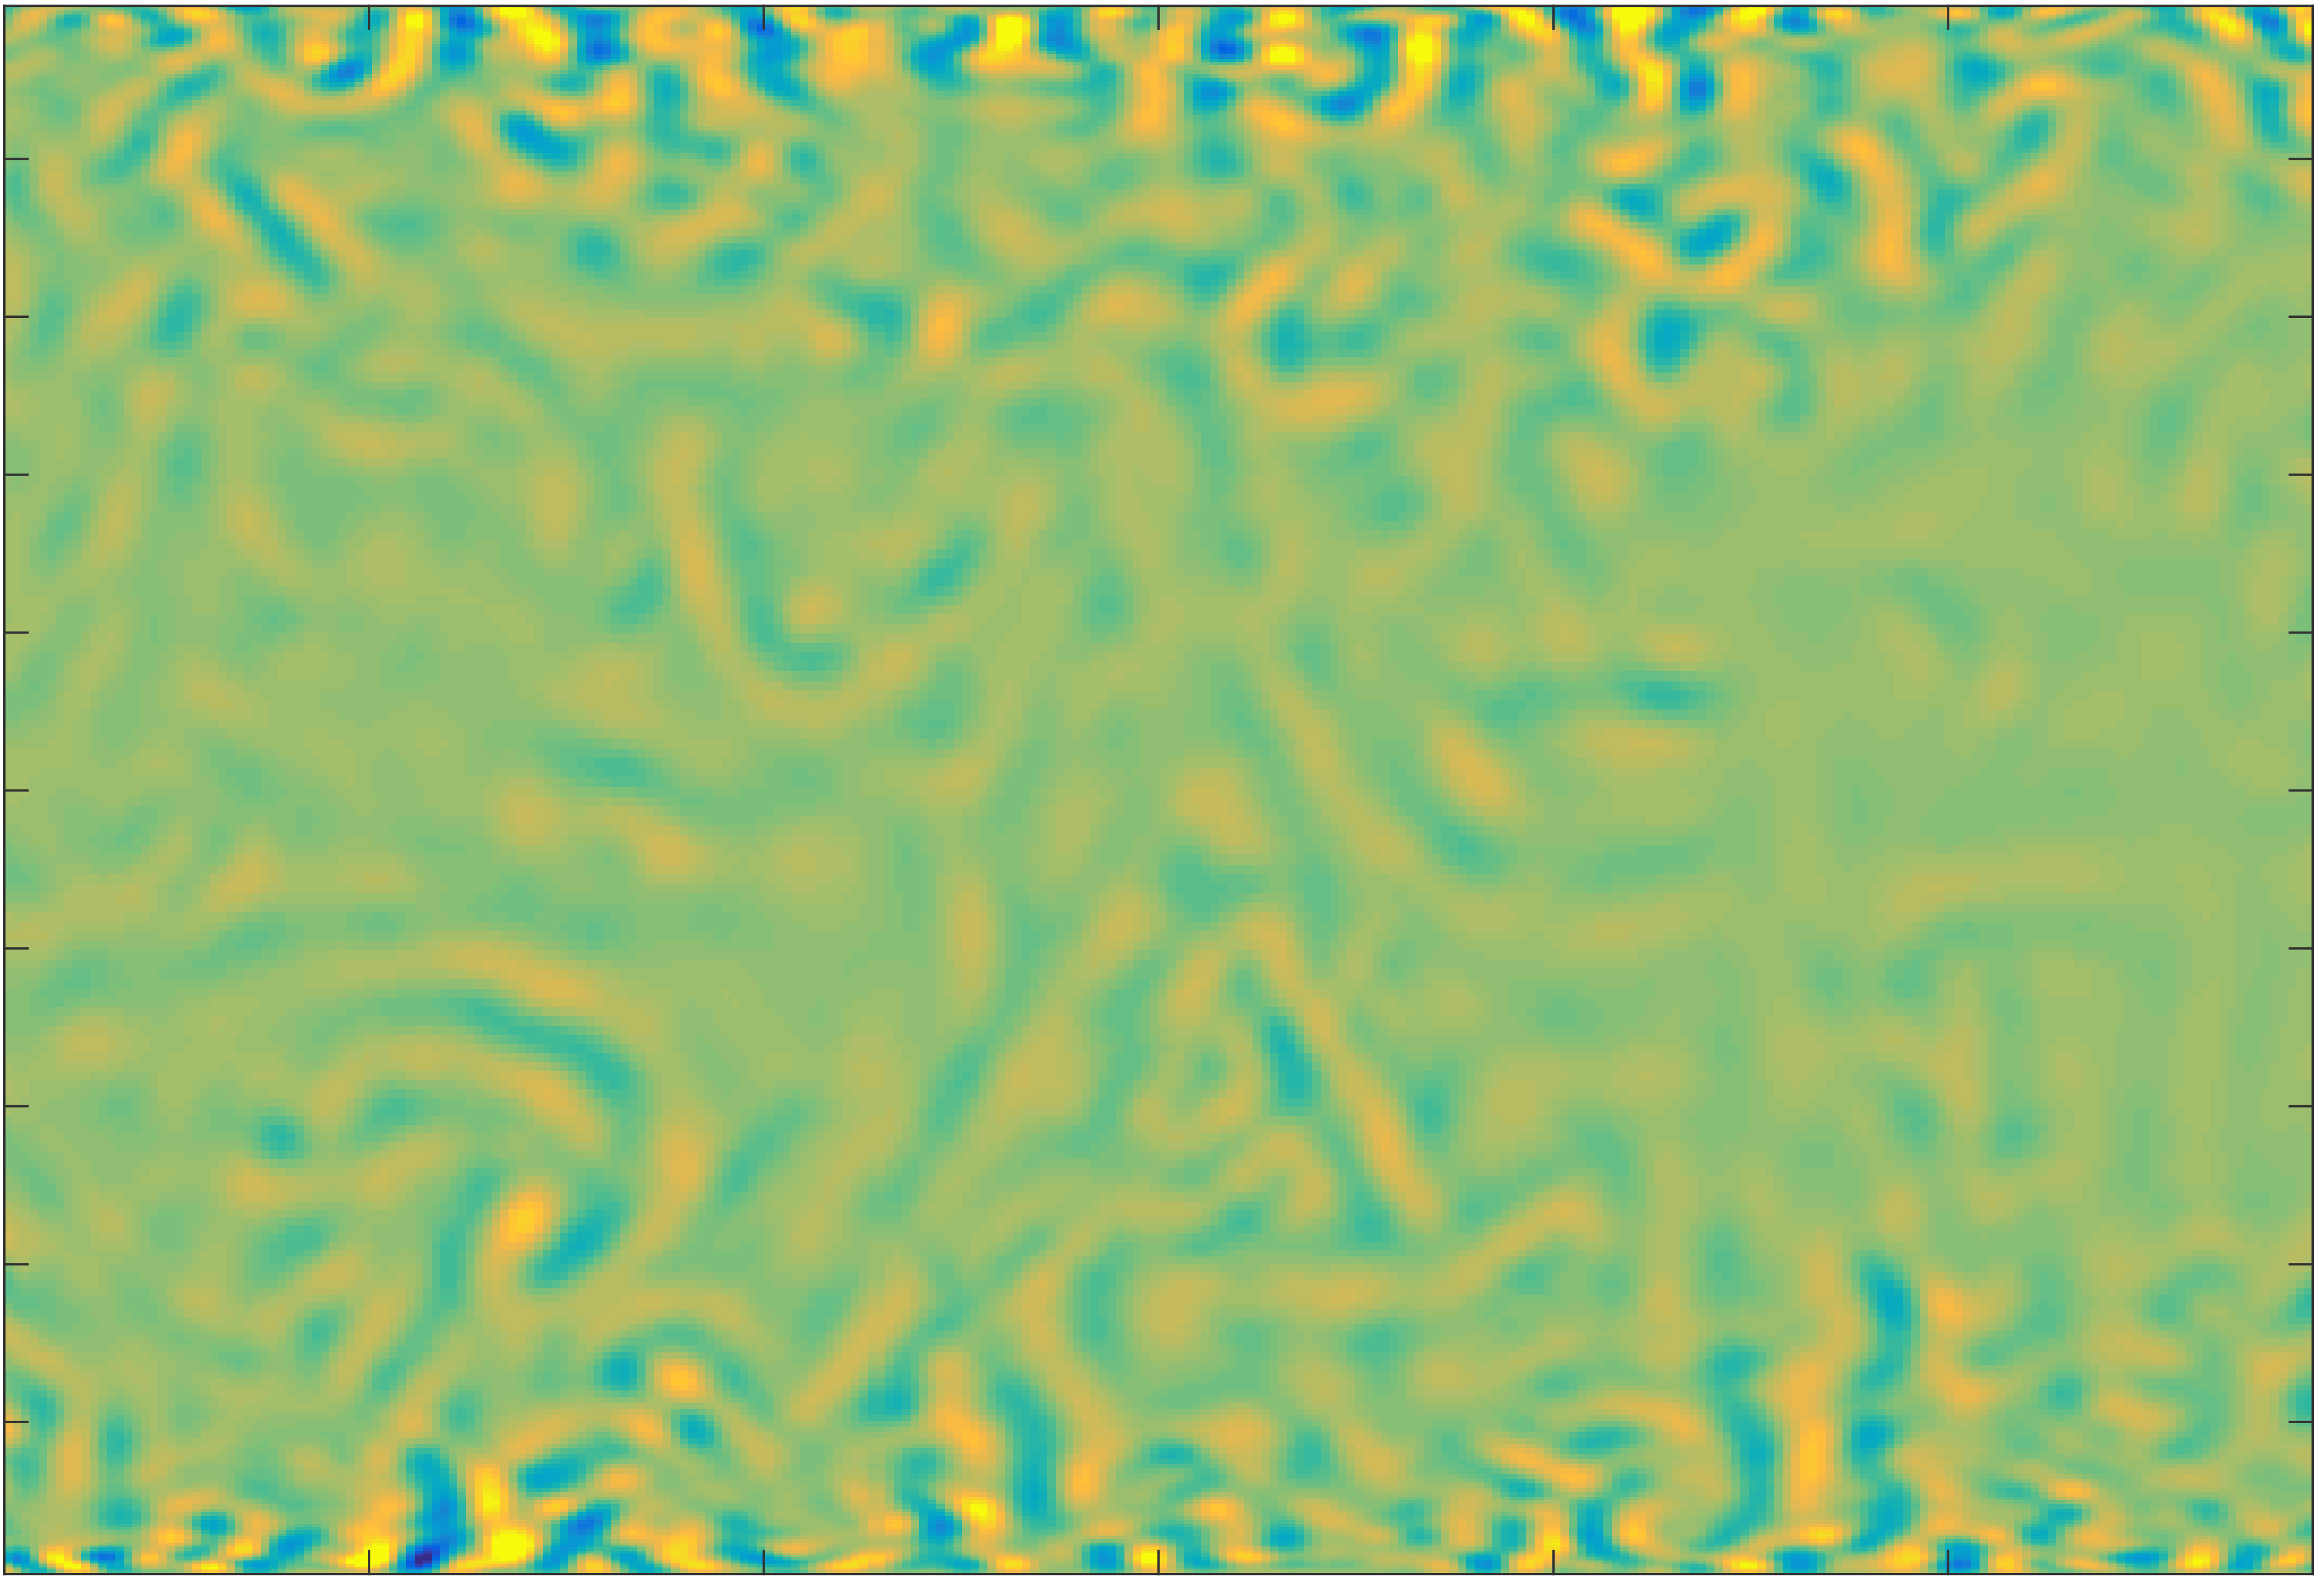
\includegraphics[height=3.75cm,valign=t]{./figures/turbulence/Umid.png}
		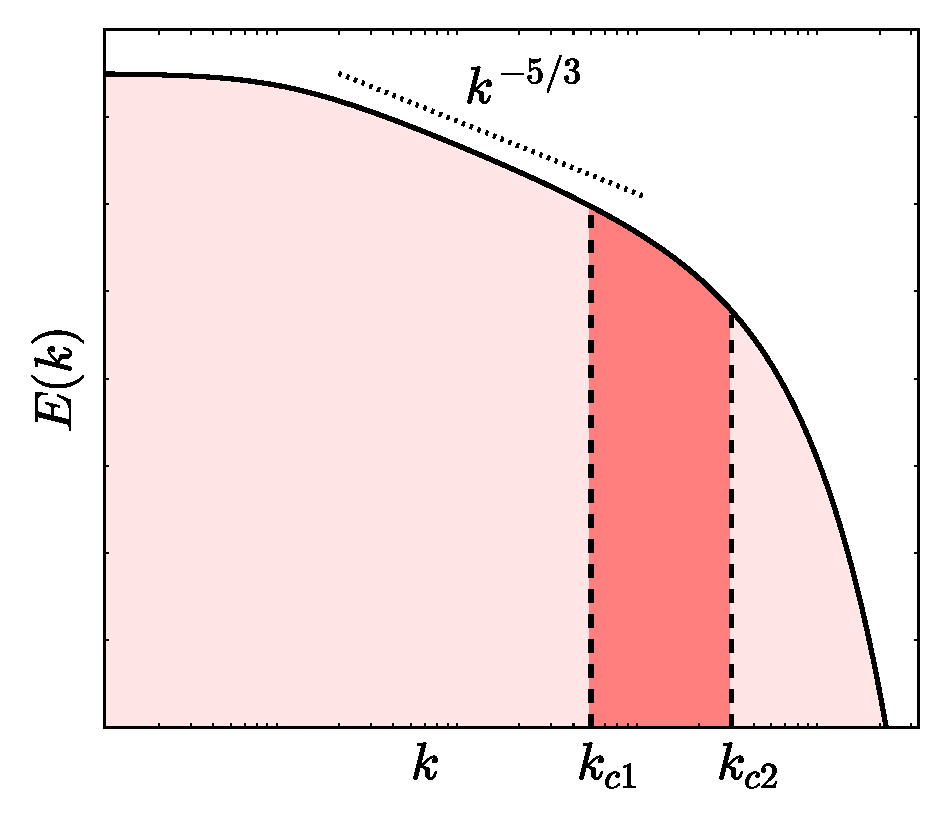
\includegraphics[height=4.1cm,valign=t]{./figures/turbulence/turbulence_spectra_variousranges2.eps}
		\caption*{Sample streamwise velocity field of a channel flow ($ Re_\tau = 550$) and a synthesized spectrum (mid scales)}
	\end{figure}
	\onslide<5>	
	\begin{figure}
		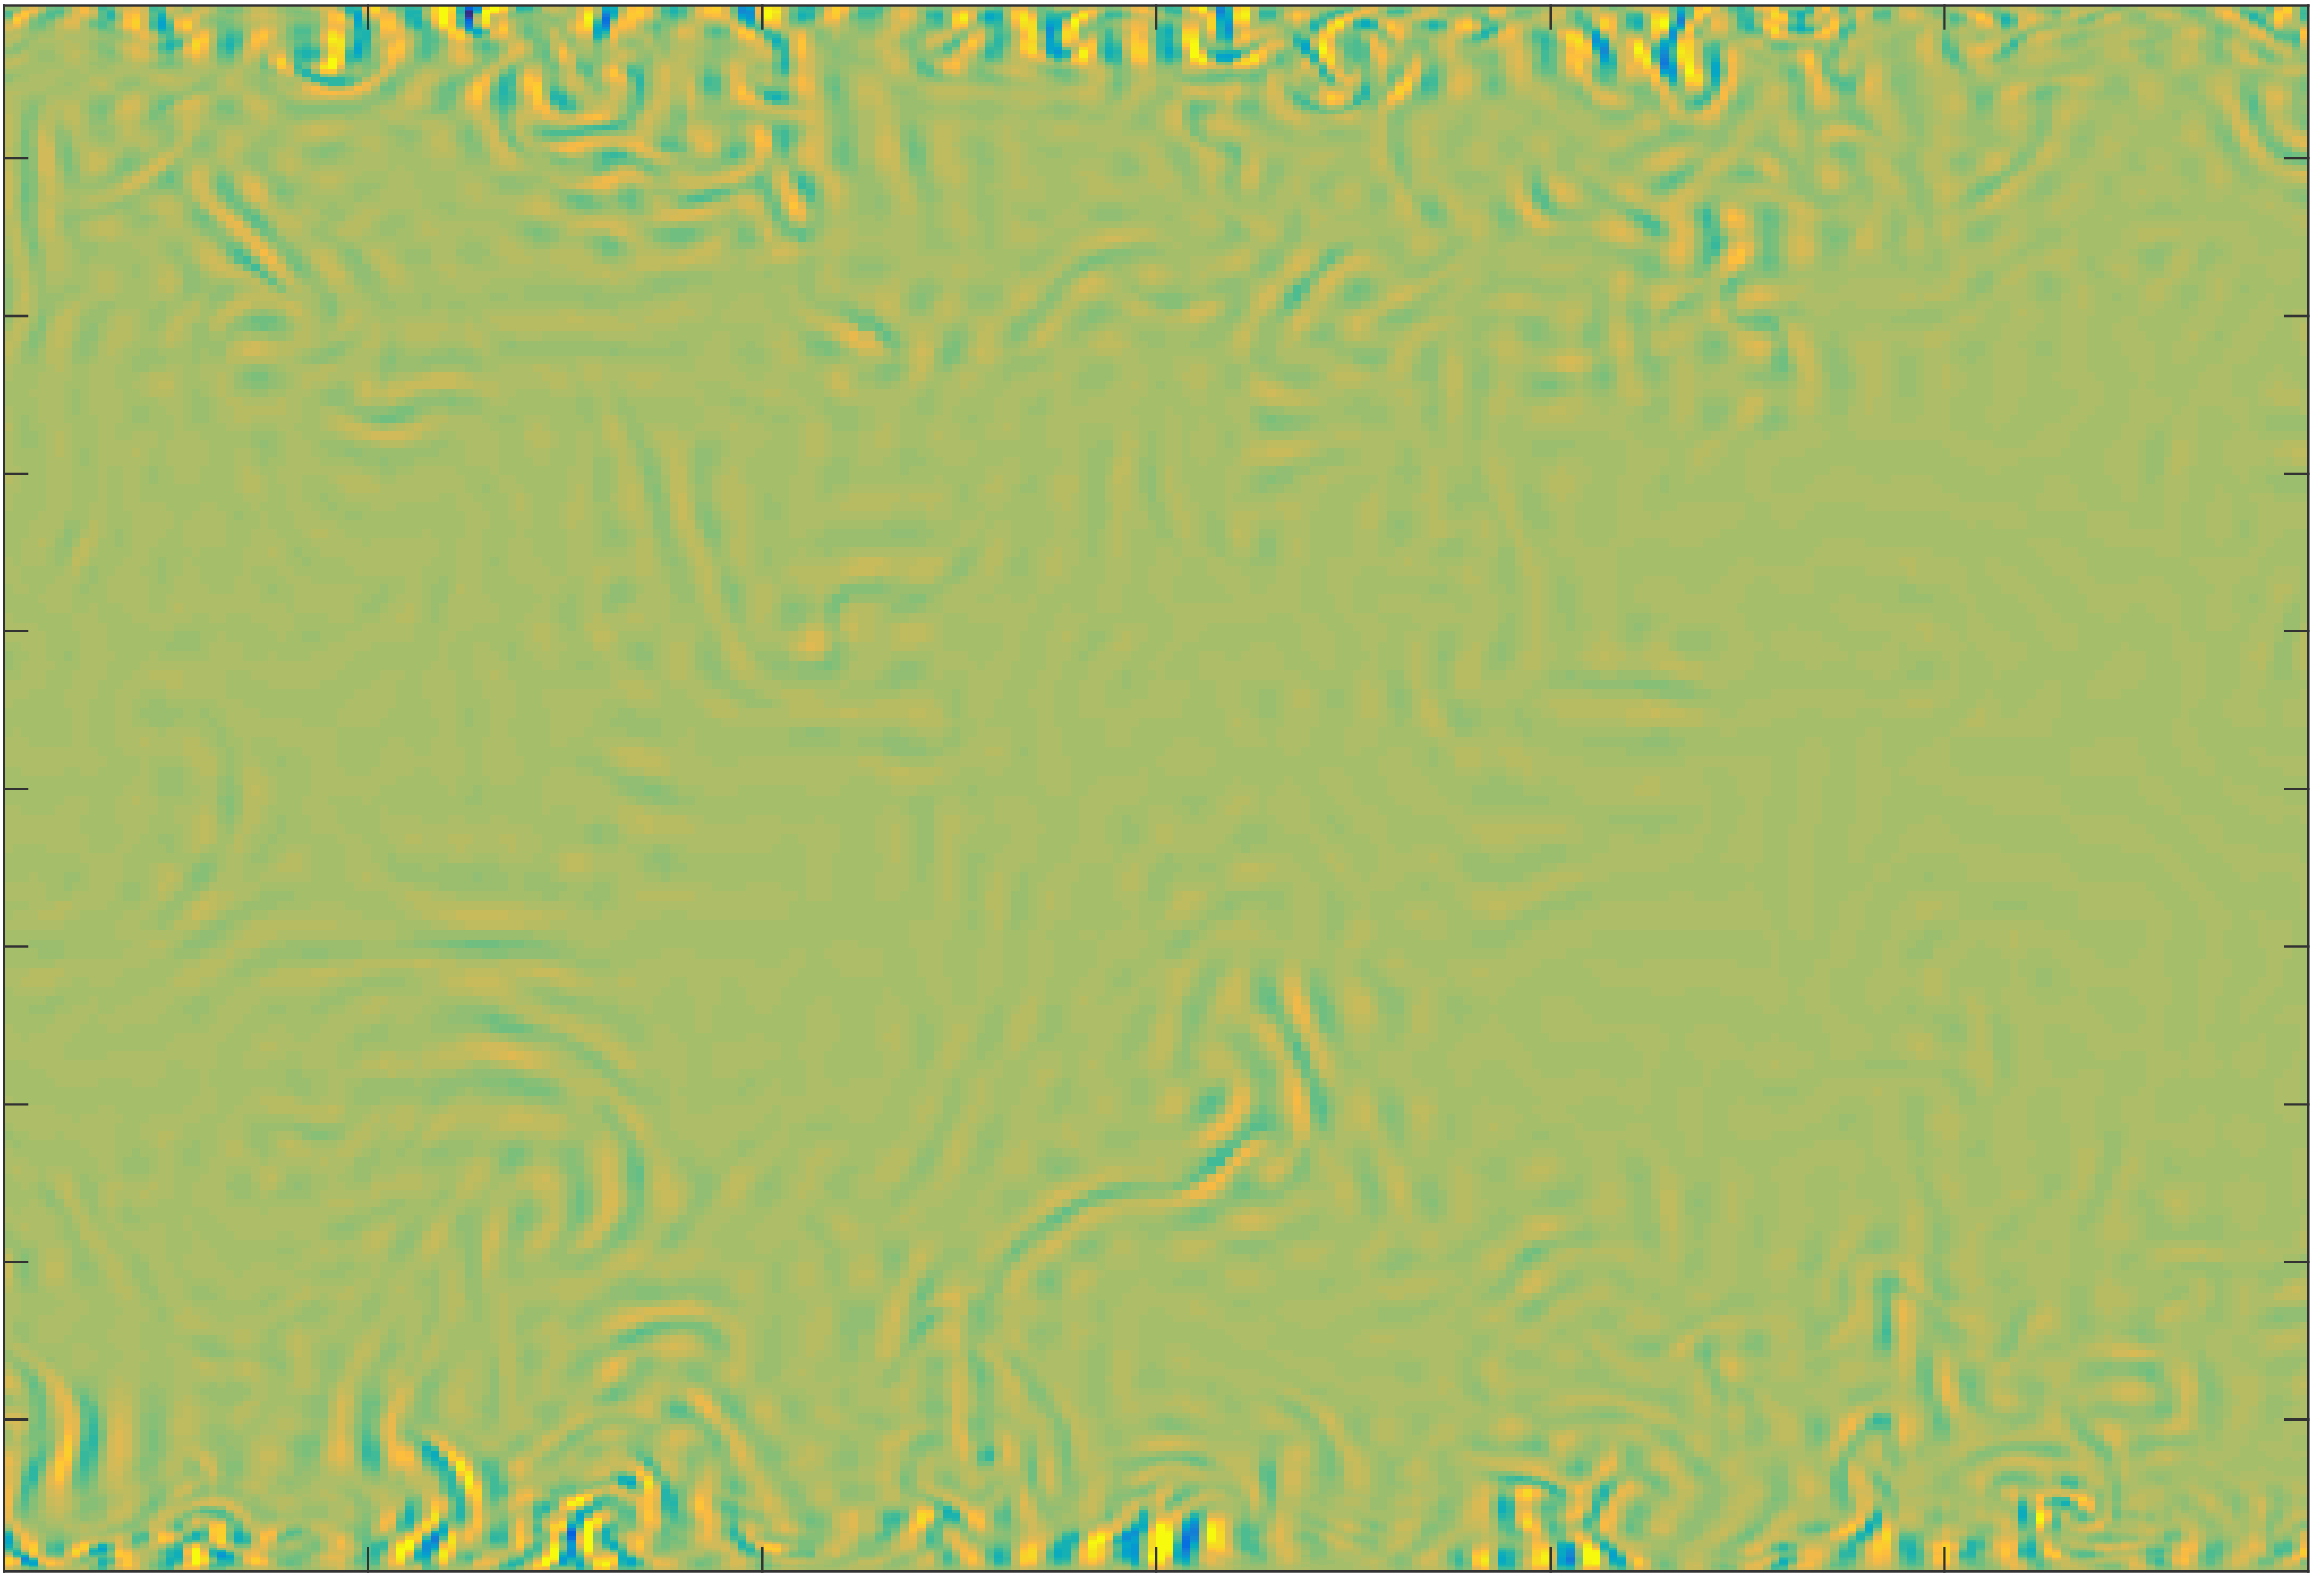
\includegraphics[height=3.75cm,valign=t]{./figures/turbulence/Usmall.png}
		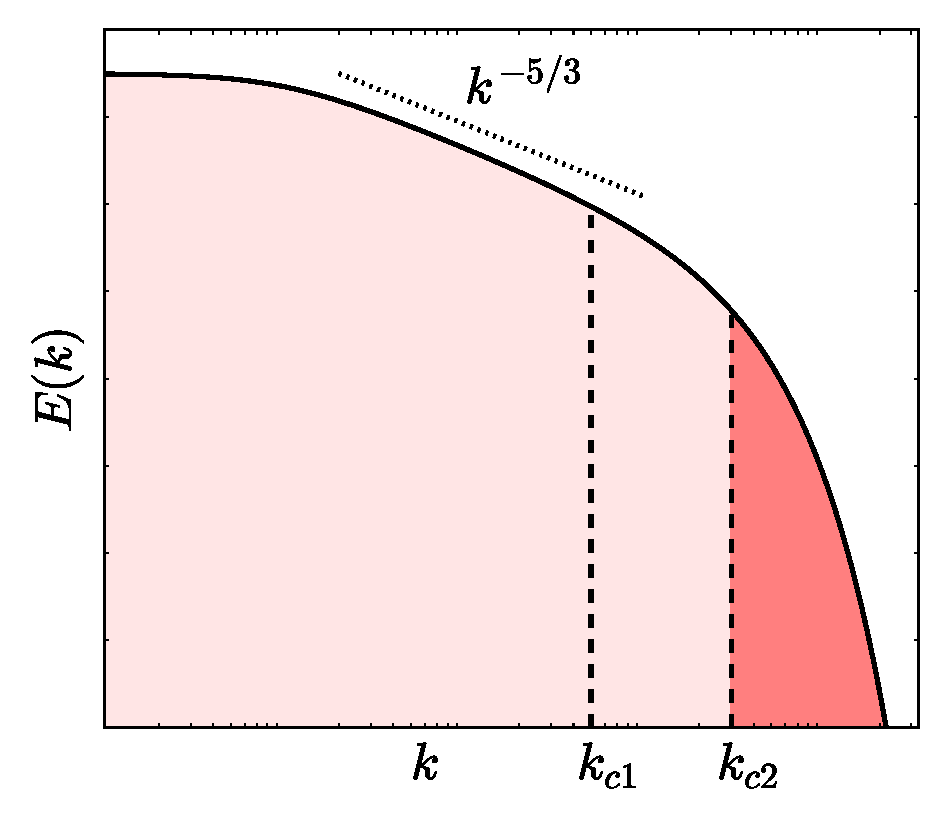
\includegraphics[height=4.1cm,valign=t]{./figures/turbulence/turbulence_spectra_variousranges3.eps}
		\caption*{Sample streamwise velocity field of a channel flow ($ Re_\tau = 550$) and a synthesized spectrum (small scales)}
	\end{figure}
	\onslide<6>	
	\begin{figure}
		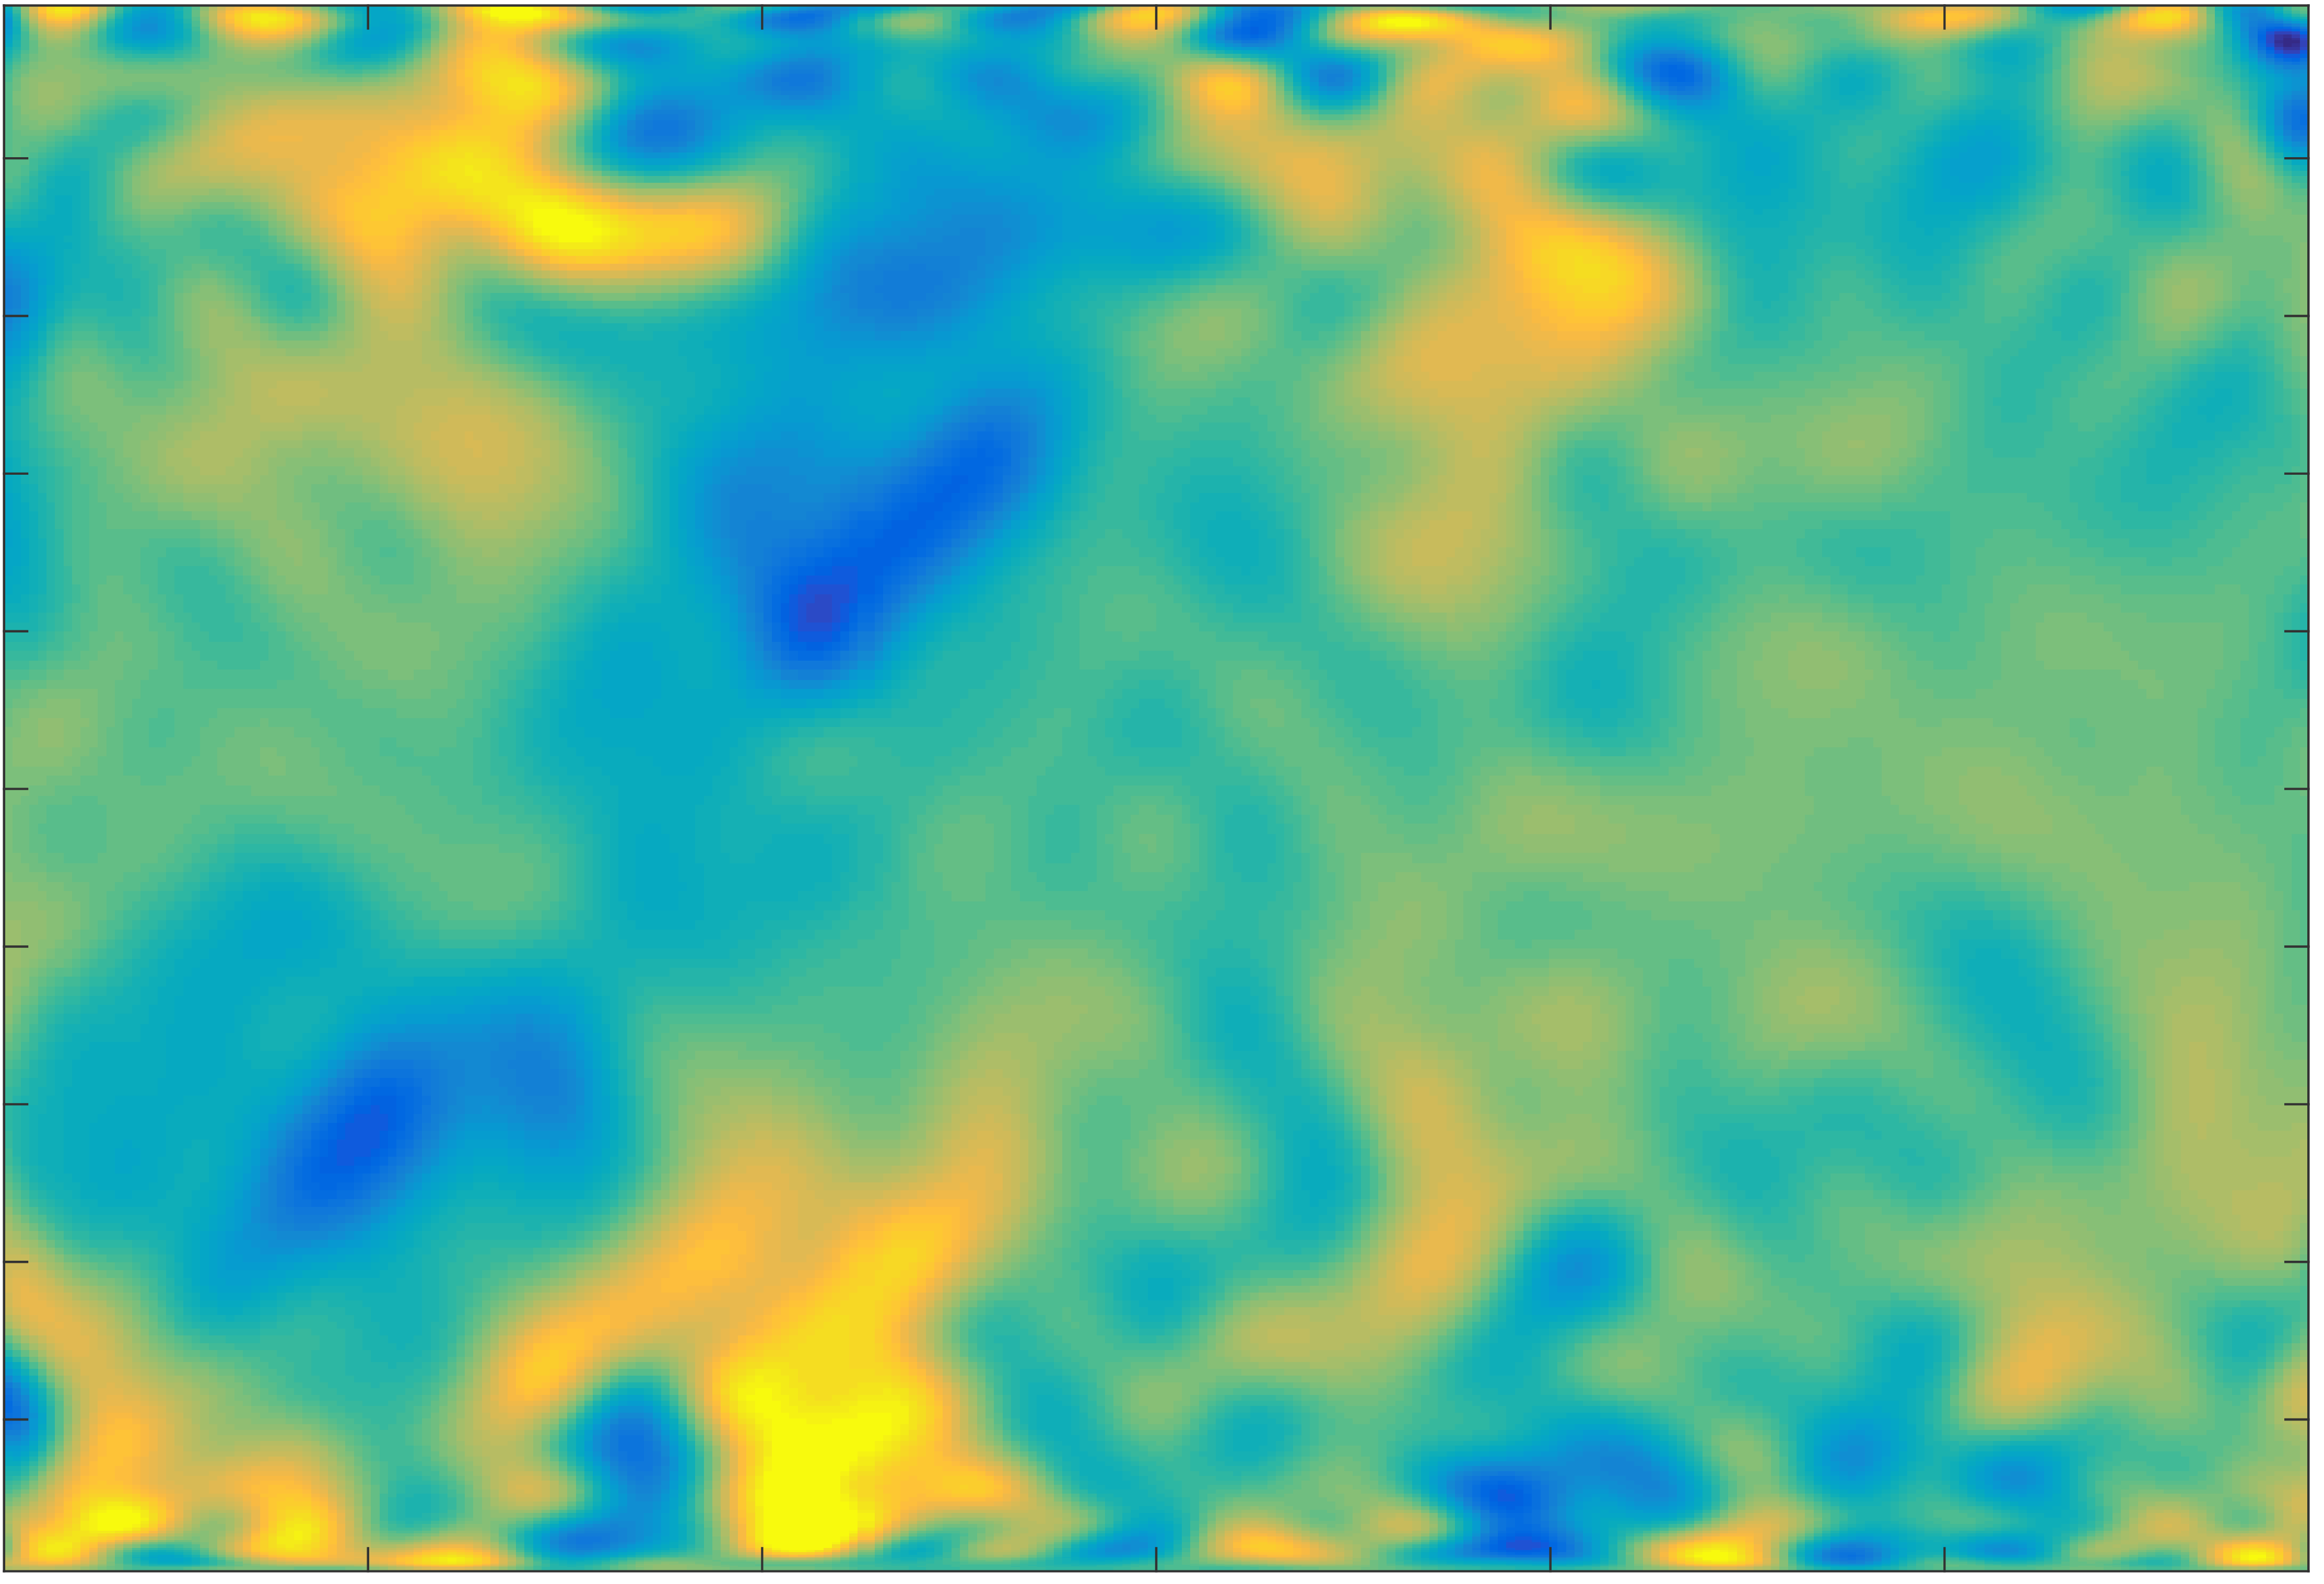
\includegraphics[height=3.75cm,valign=t]{./figures/turbulence/Ularge.png}
		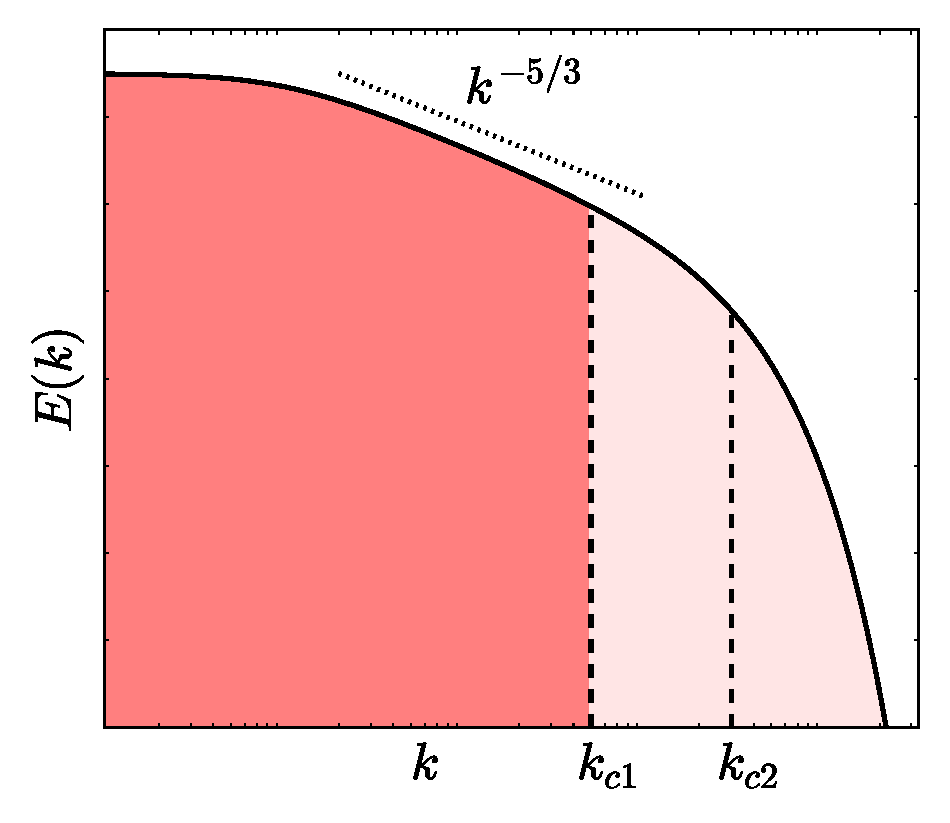
\includegraphics[height=4.1cm,valign=t]{./figures/turbulence/turbulence_spectra_variousranges1.eps}
		\caption*{Sample streamwise velocity field of a channel flow ($ Re_\tau = 550$) and a synthesized spectrum (large scales)}
	\end{figure}
	\onslide<7>	
	\begin{figure}
		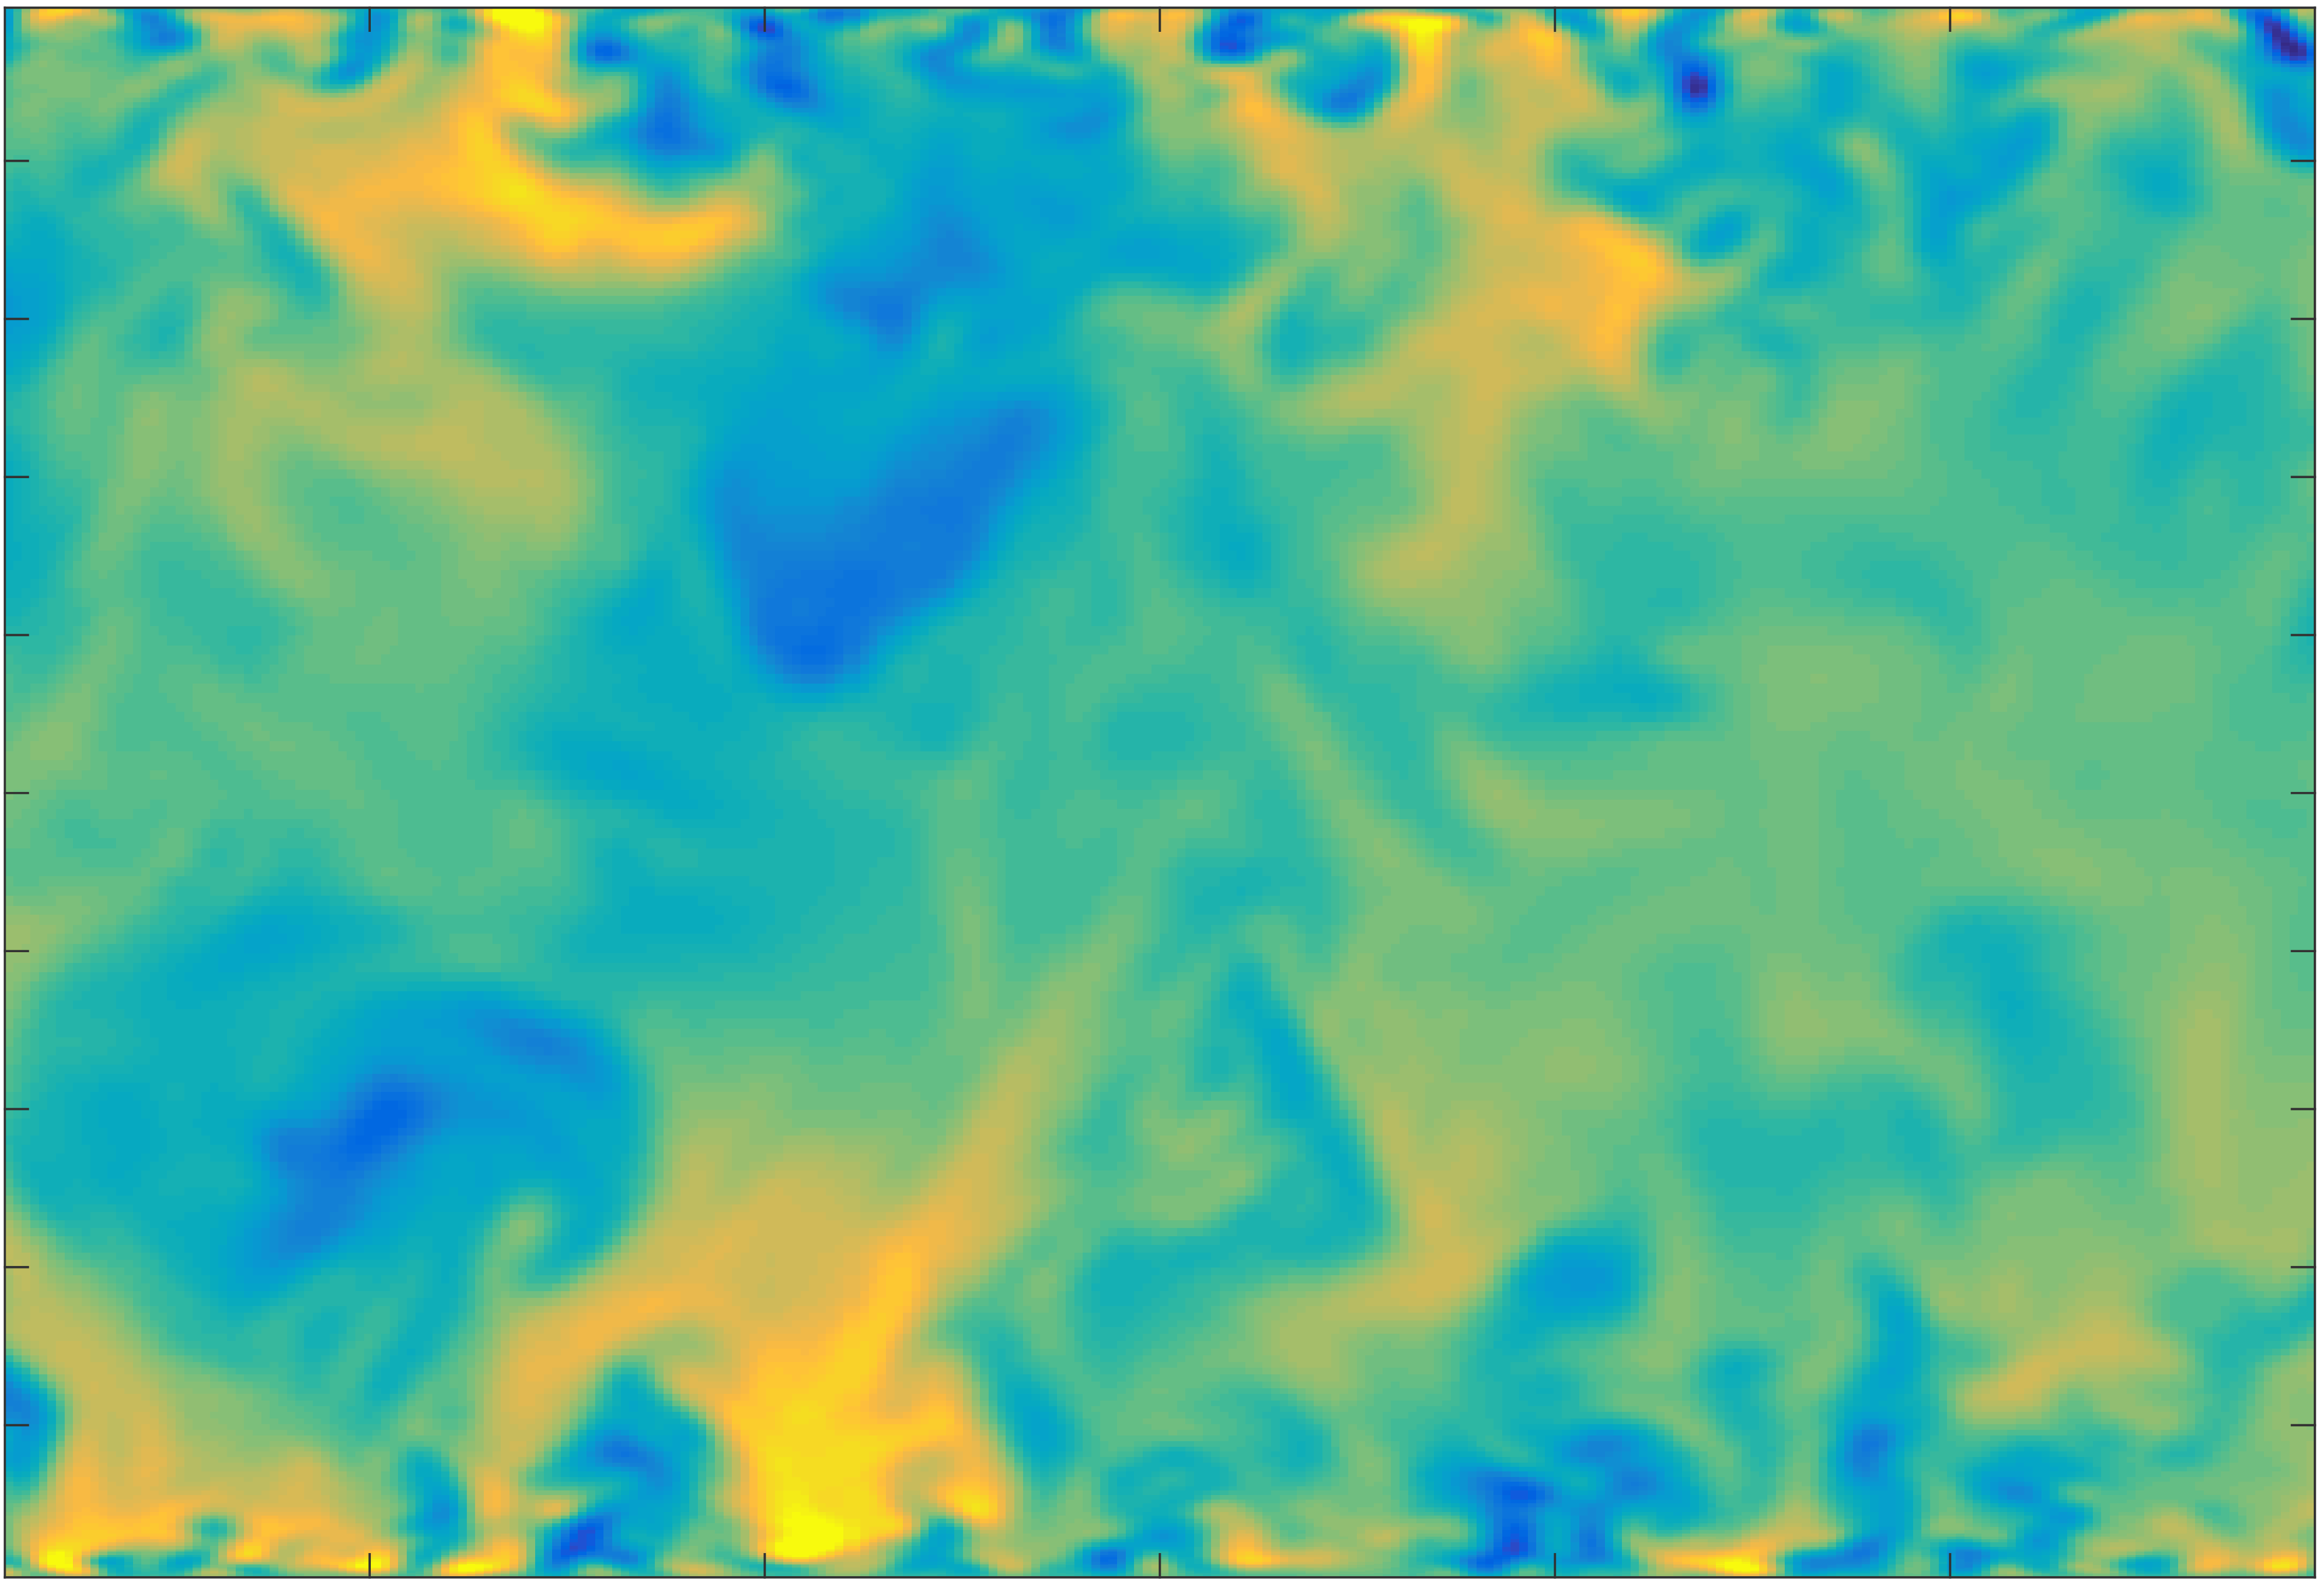
\includegraphics[height=3.75cm,valign=t]{./figures/turbulence/Ulargemid.png}
		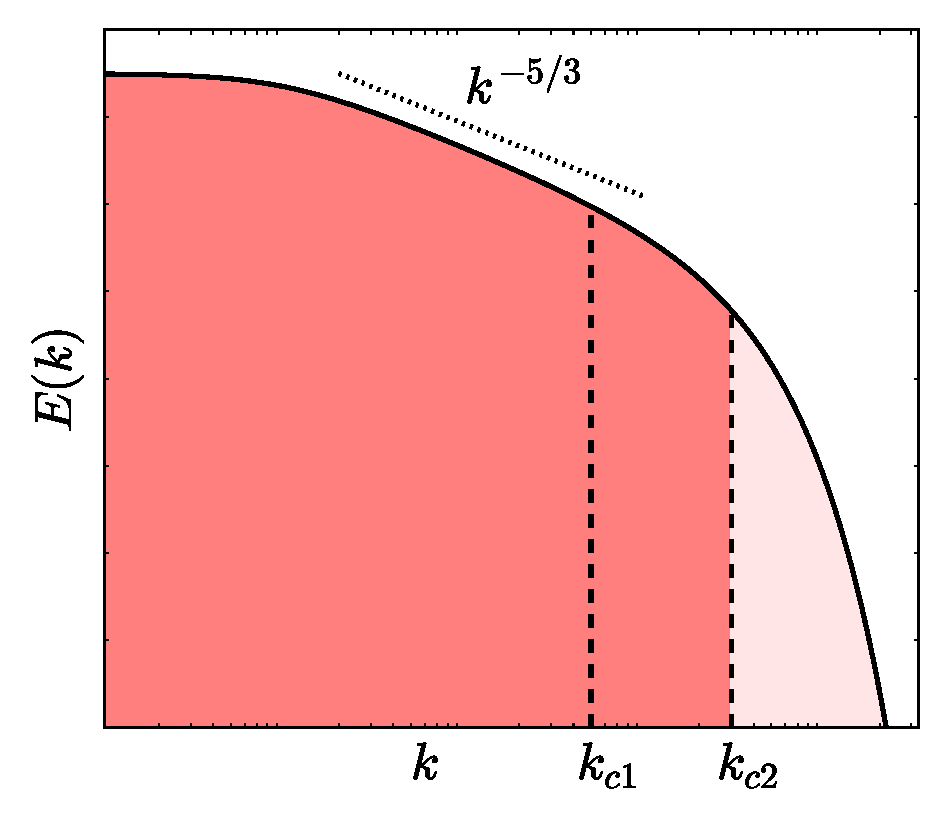
\includegraphics[height=4.1cm,valign=t]{./figures/turbulence/turbulence_spectra_variousranges12.eps}
		\caption*{Sample streamwise velocity field of a channel flow ($ Re_\tau = 550$) and a synthesized spectrum (large scales)}
	\end{figure}		
	\end{overprint}
\end{frame}

\begin{frame}
\frametitle{Importance of small scales}
	\begin{itemize}
		\item Better insight on turbulence physics (dissipation, coherent structures)
		\item Validation of turbulence models (Large Eddy Simulation)
	\end{itemize}
	\pause
	\begin{overprint}
	\onslide<2>	
	\begin{figure}
		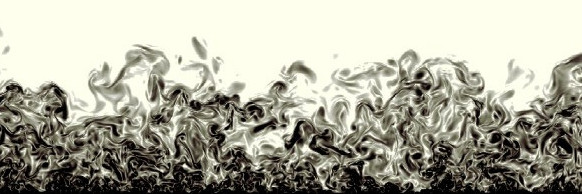
\includegraphics[width=.9\textwidth]{./figures/turbulence/nearwallturb.jpg}
		\caption*{Turbulent boundary layers (photo credit: Juan A. Sillero)}
	\end{figure}
	\onslide<3>	
	\begin{figure}
		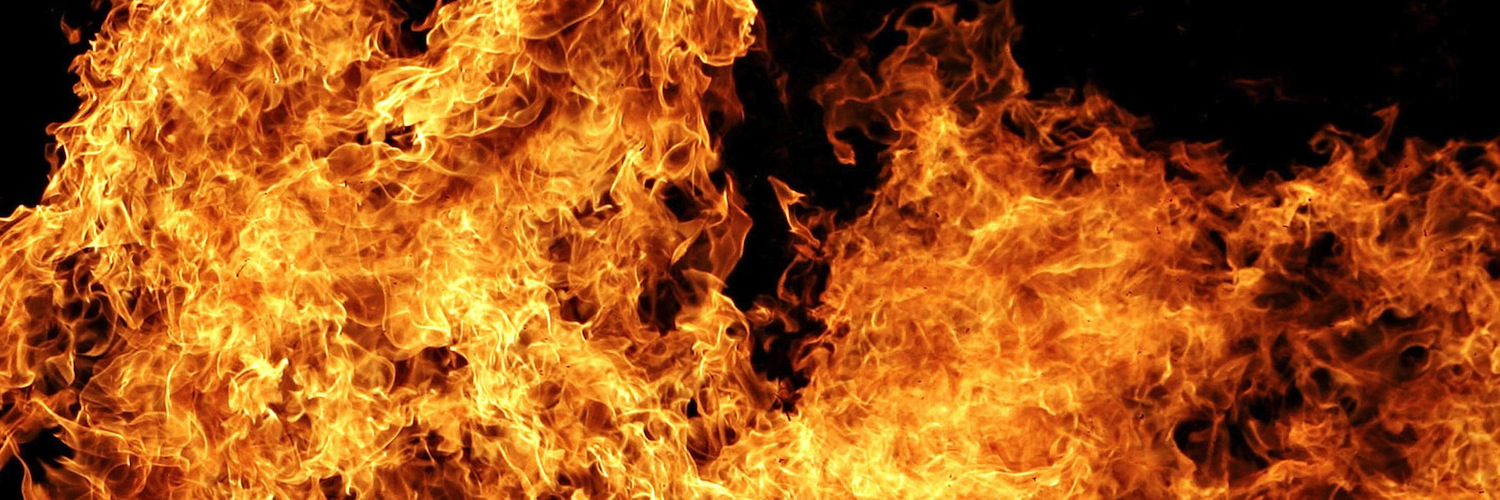
\includegraphics[width=.9\textwidth]{./figures/turbulence/flame.jpg}
		\caption*{Turbulent combustion and reacting flows (photo credit: TESLa, Colorado University)}
	\end{figure}
	\end{overprint}
\end{frame}

\begin{frame}
\frametitle{Motivations of the thesis}
	\begin{block}{\textbf{Problem}: cannot access a full range of scales}
		\begin{itemize}
			\item \textbf{\color{red}Experiments:}
				\begin{itemize}
					\item \textbf{Optical measurement} (PIV, PTV): compromise between frequency, resolution and field-of-view
					\item \textbf{Hot wire anemometer} (HWA): high frequency but point-measurement
				\end{itemize}
			\item \textbf{\color{red}Simulations:} only accessible from Direct Numerical Simulation, but
				\begin{itemize}
					\item limited to low to moderate $ Re $ and/or simple geometries
					\item excessive computational cost to converge statistics
				\end{itemize}
		\end{itemize}
	\end{block}	
	\vfill
	\begin{block}{\textbf{Our main objectives}:}
		\begin{itemize}
			\item Computational methods to reconstruct partly unresolved scales
			\item Model assessment using numerical database
		\end{itemize}
	\end{block}	
\end{frame}

\begin{frame}
\frametitle{Numerical experiment setup}
	\begin{block}{\textbf{Setup of complementary measurements}:}
		\begin{itemize}
			\item High-Time-Low-Space (\textbf{HTLS}) of size $ \dimsl \times \dimth $
			\item Low-Time-High-Space (\textbf{LTHS}) of size $ \dimsh \times \dimtl $ ($ \dimsl \ll  \dimsh, \dimtl \ll  \dimth$)
		\end{itemize}
	\end{block}
	\vfill
	\begin{figure}
	\centering 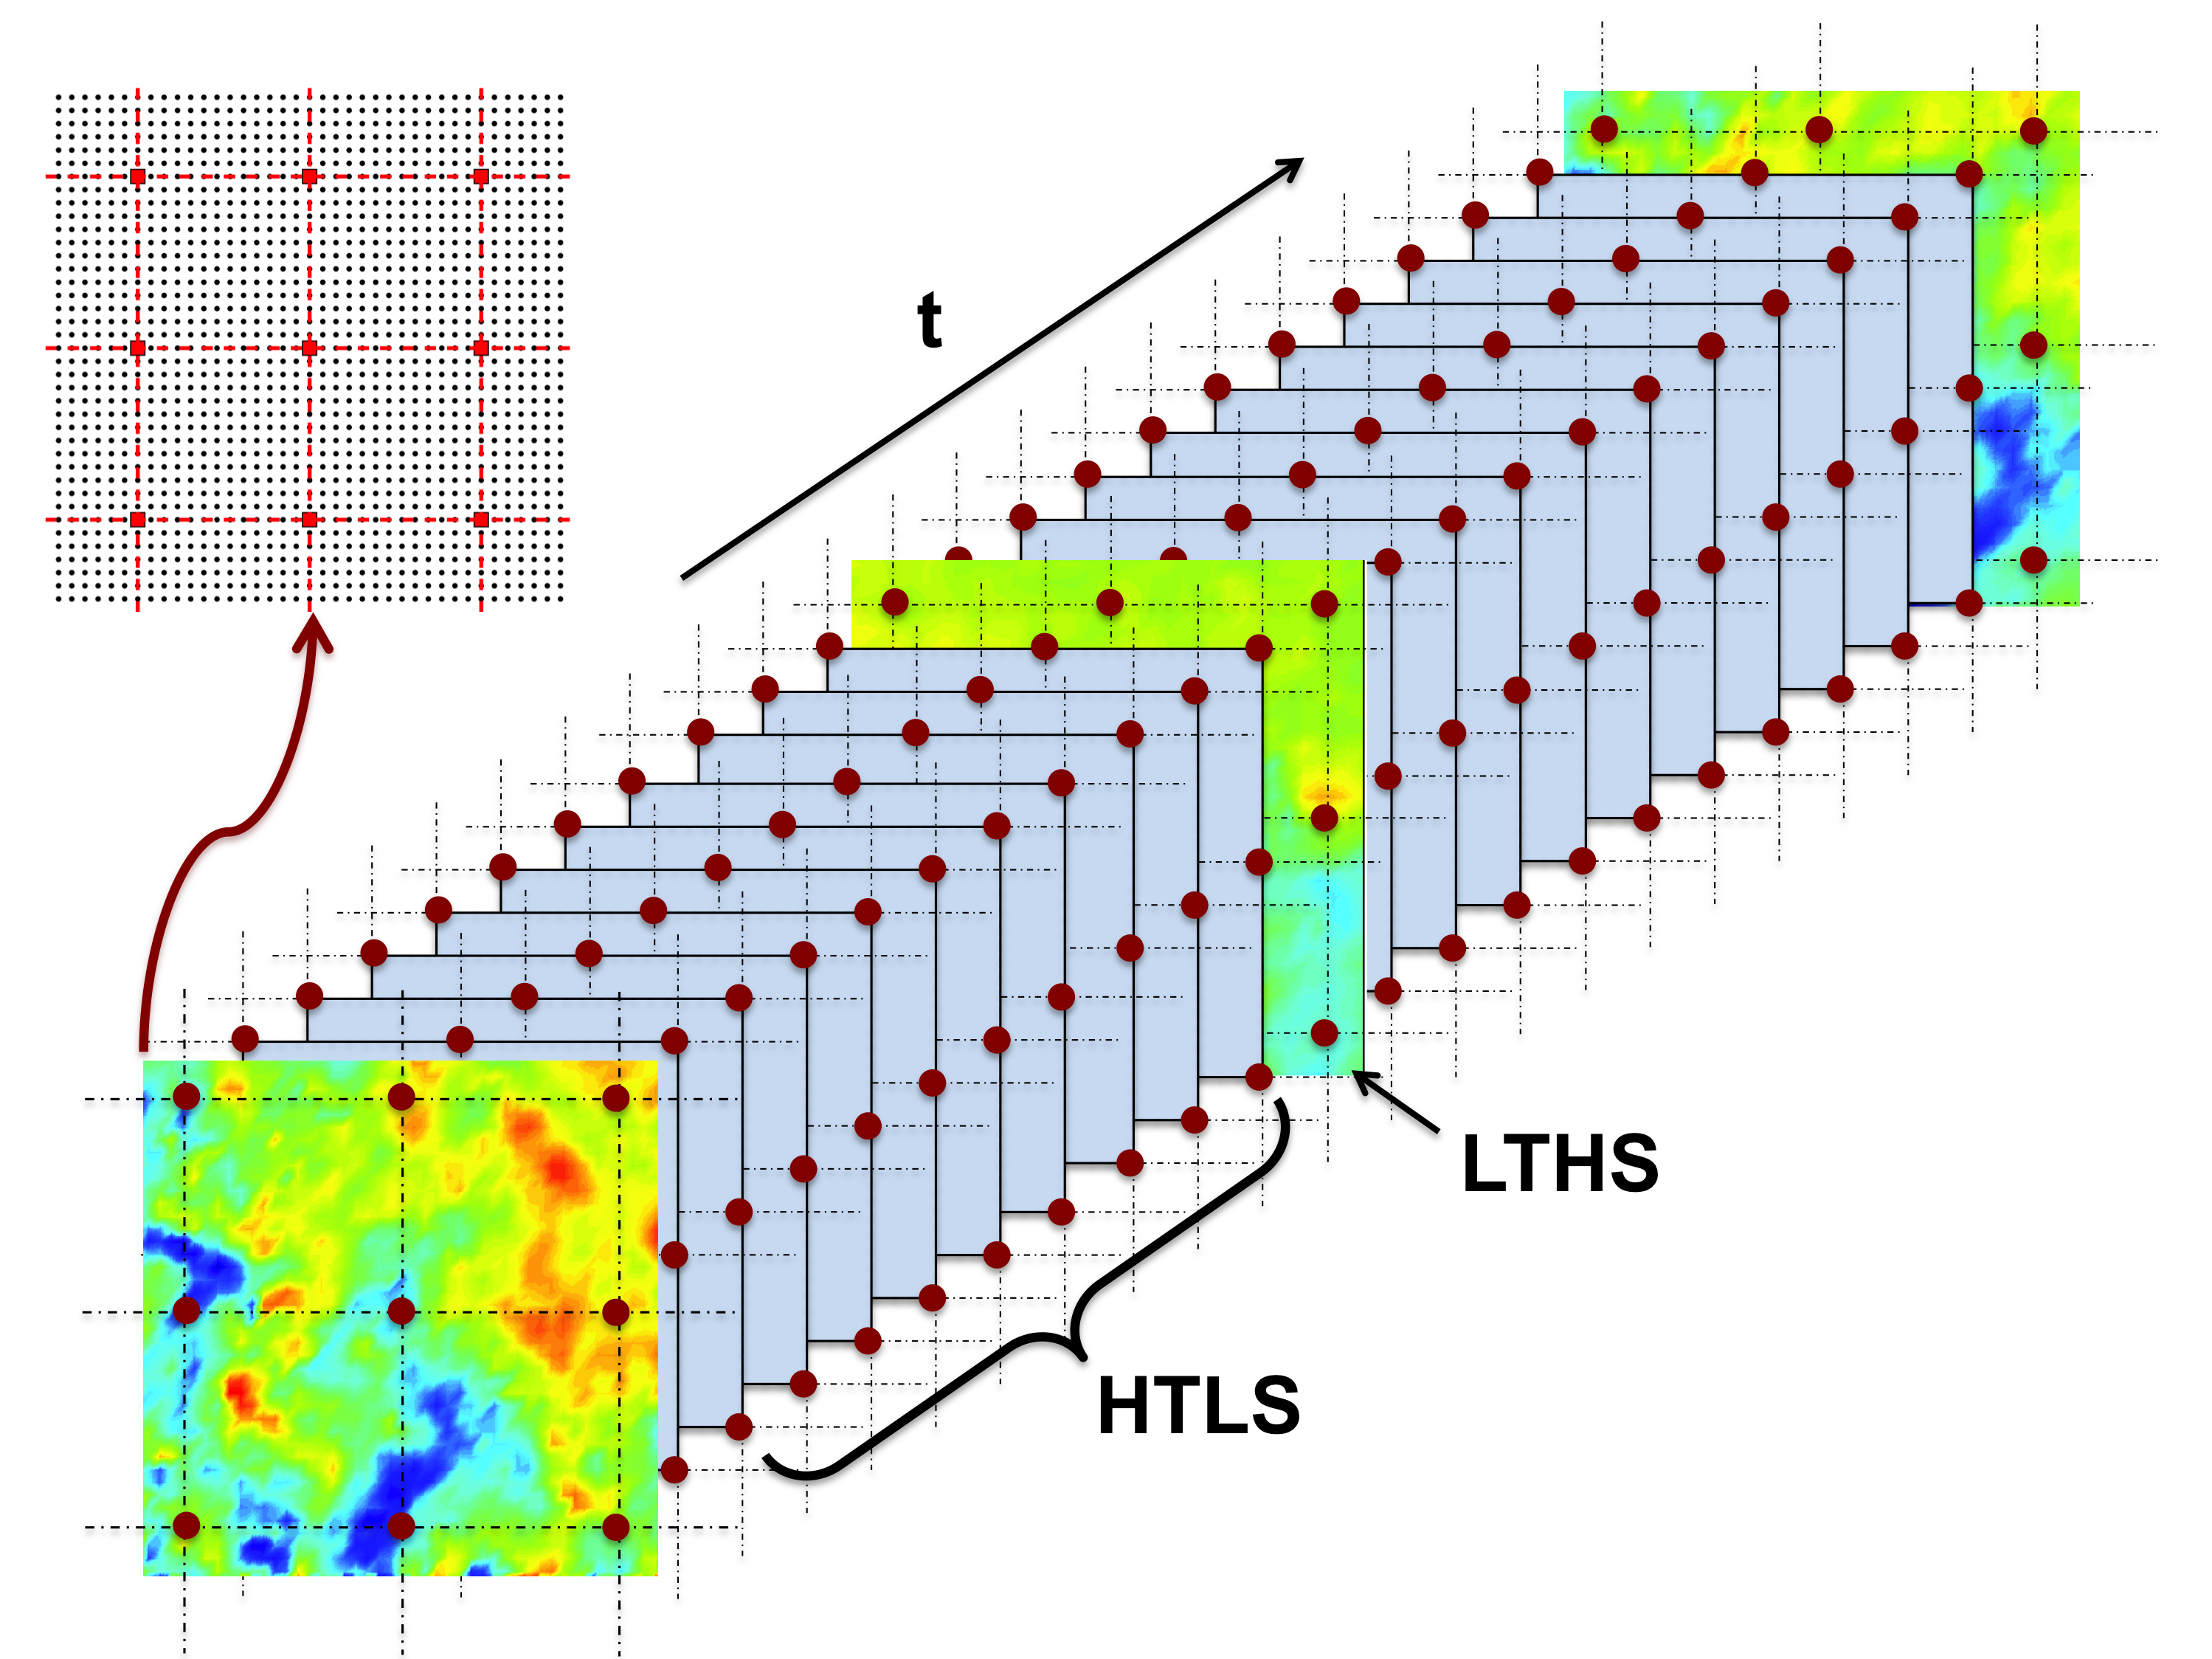
\includegraphics[width=0.58\textwidth]{./figures/experimentalsetup/experiment_setup.png}
	\end{figure}
\end{frame}

\begin{frame}
\frametitle{Example: WALLTURB project {\footnotesize \cite{coudert2011double}}}
	\vspace{-0.1cm}
	\begin{itemize}
		\item Complementary measurements: \textbf{HWA} as \textbf{HTLS} ($ 11 \times 13 $, 30 kHz), \\ \textbf{PIV} as \textbf{LTHS} ($ 143 \times 161 $, 4 Hz)
		\item Reconstruct \textbf{HTHS} ($ 143 \times 161 $, 30 kHz) using regression {\footnotesize \cite{Dekou2016}}
	\end{itemize}
	\vspace{-0.2cm}
	\begin{figure}
	\centering 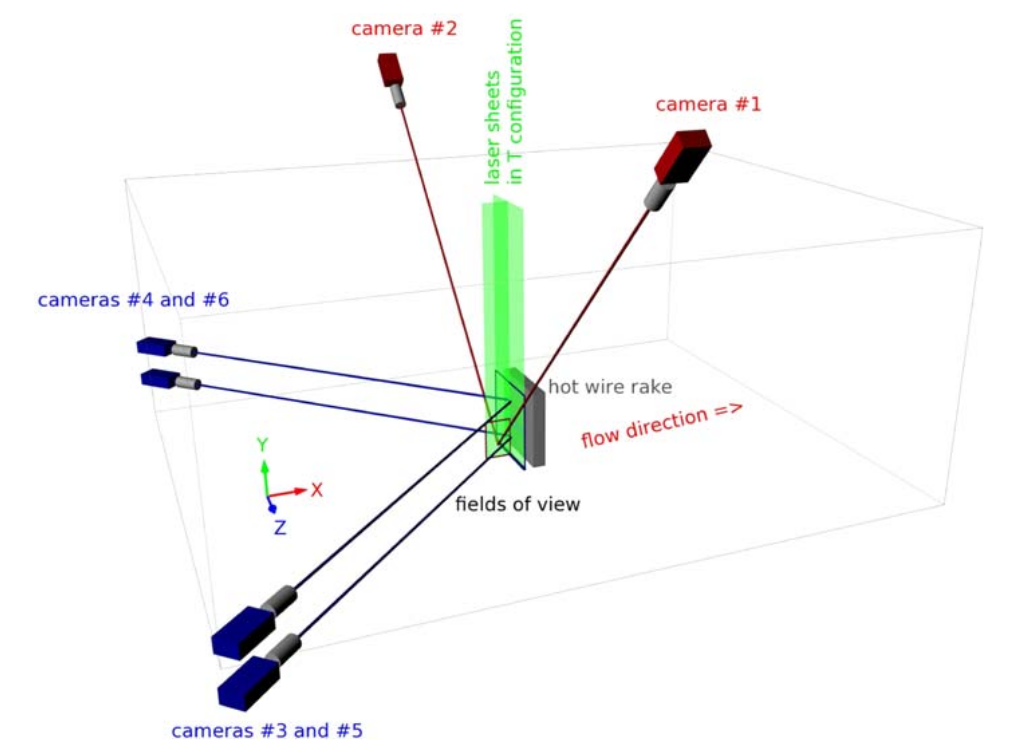
\includegraphics[width=0.6\textwidth]{./figures/experimentalsetup/Windtunnel4.png}
	\end{figure}		
\end{frame}

\subsection[The two problems]{The two addressed problems}
\begin{frame}
\frametitle{Problem definition: inverse problem}
	\begin{figure}
		\begin{overprint}
			\onslide<1>	
			\centerline{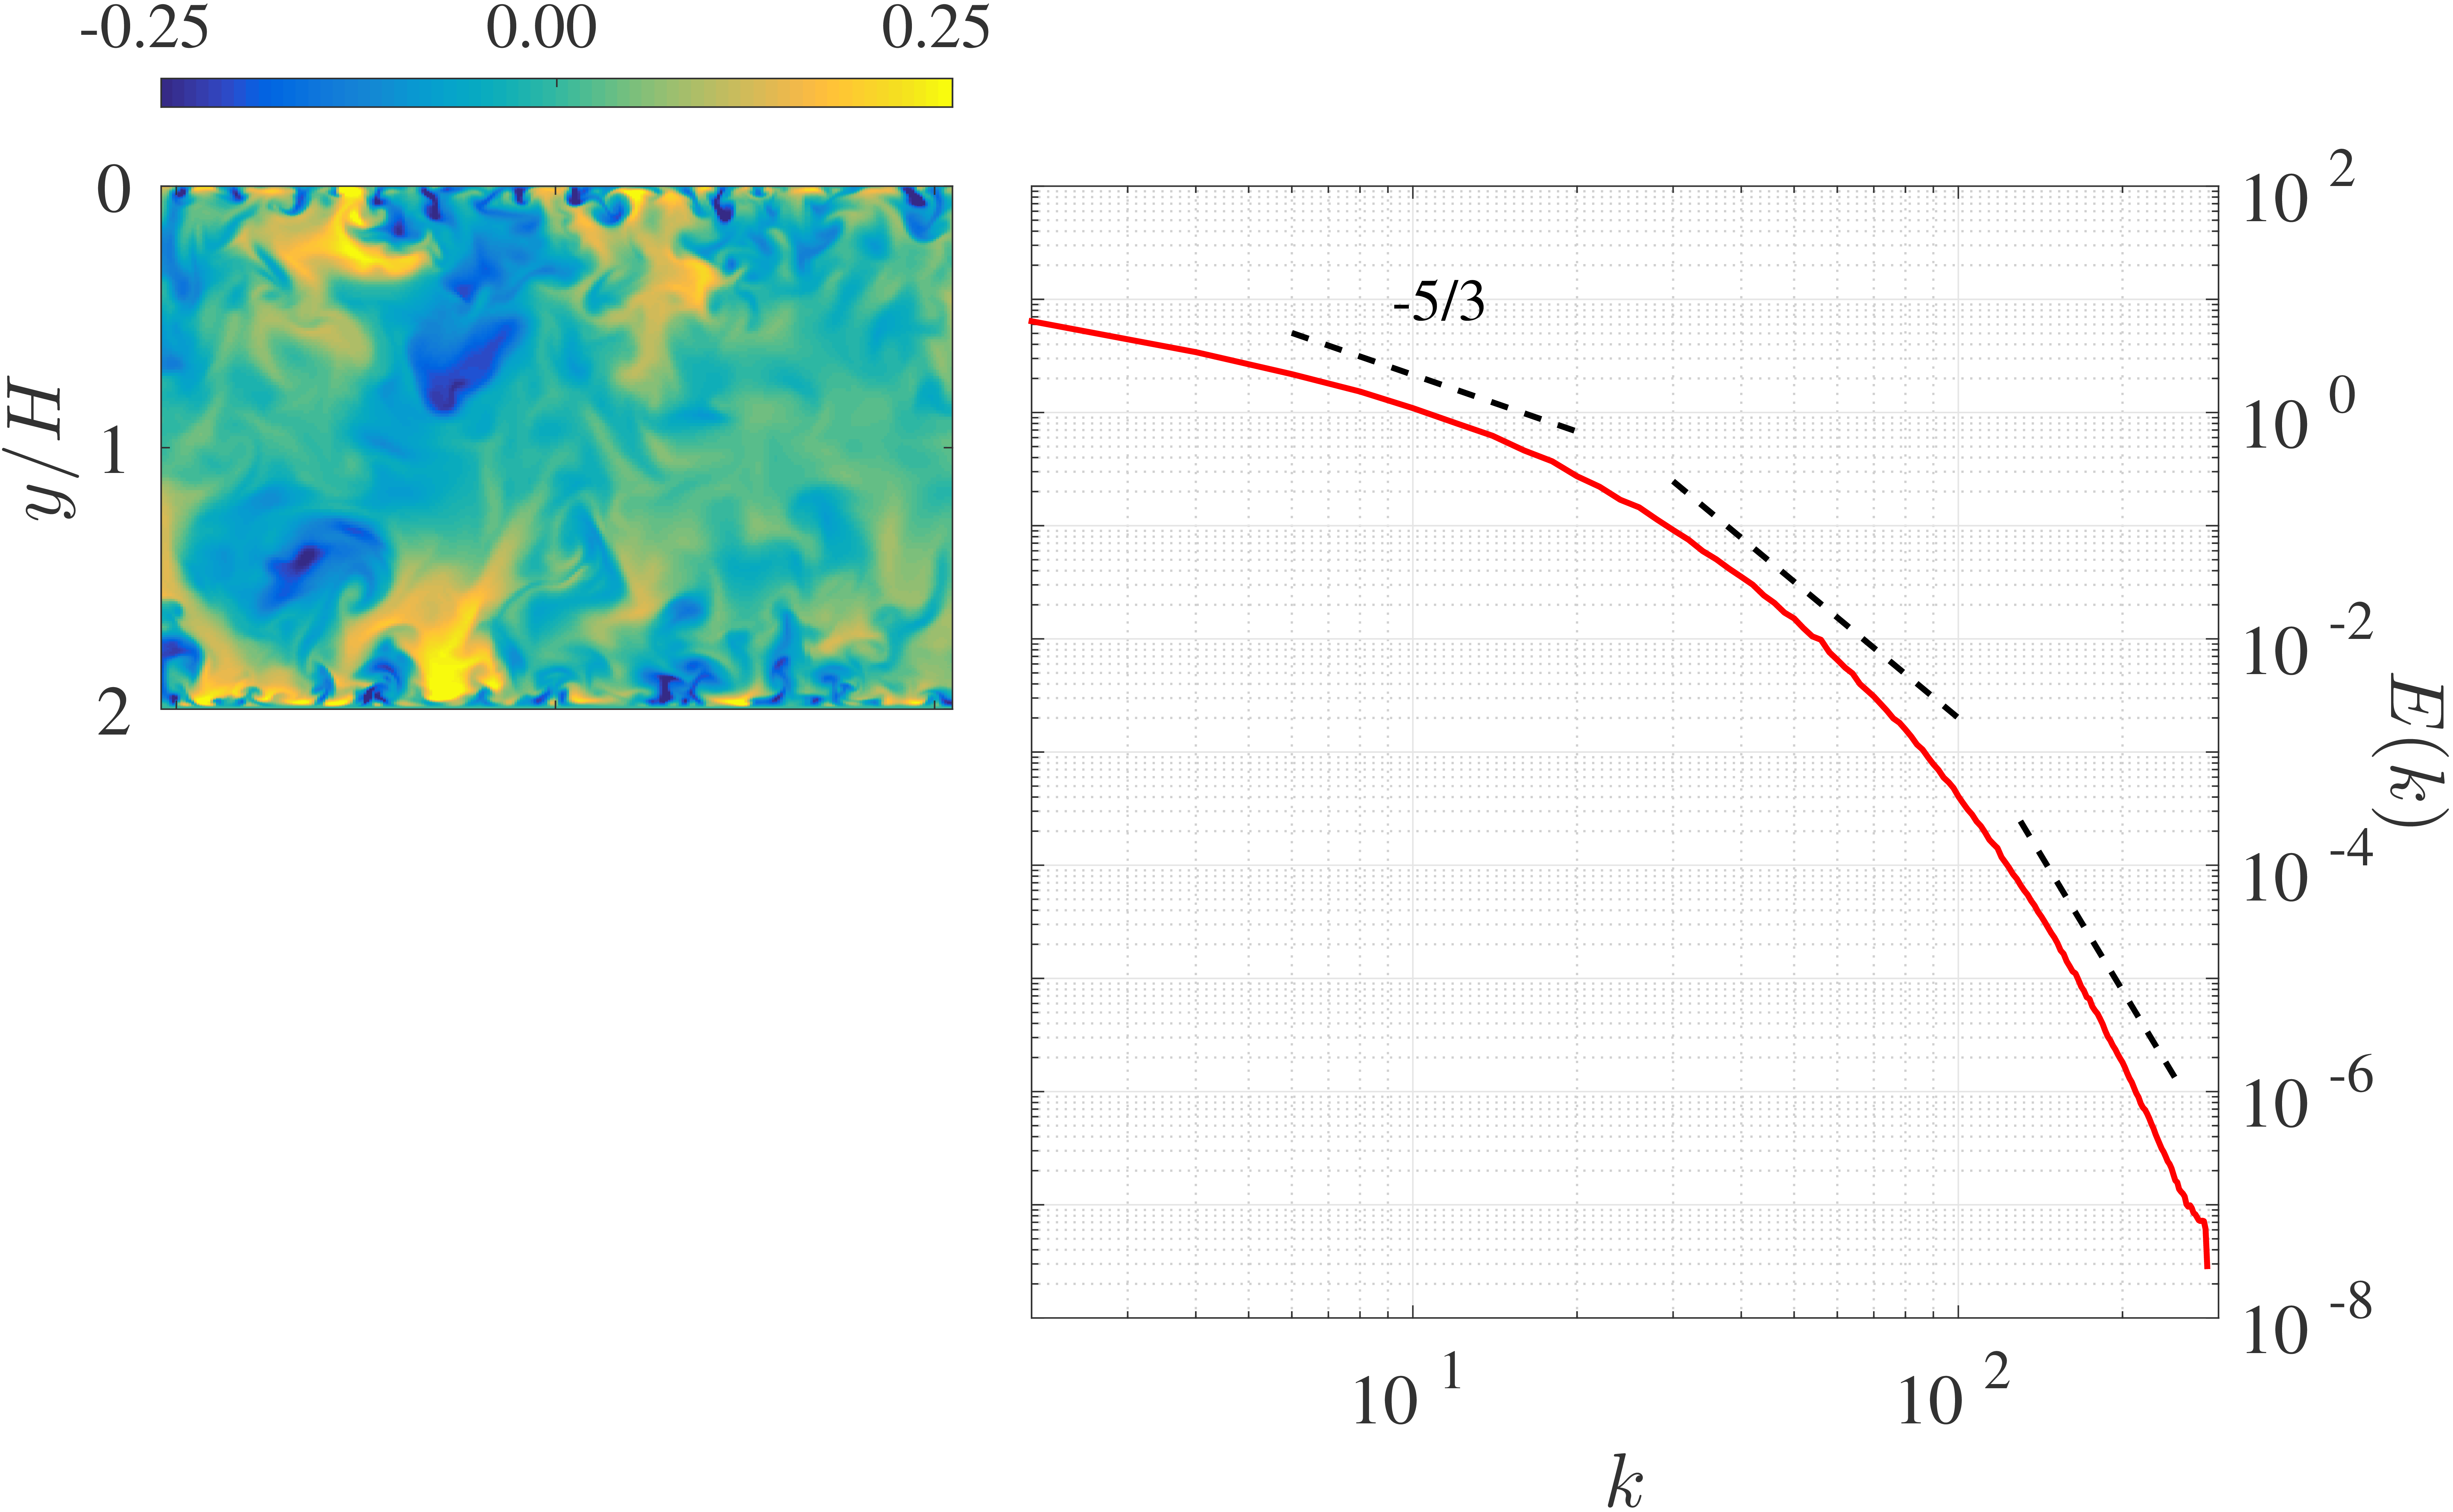
\includegraphics[width=0.85\textwidth]{./figures/turbulence/channel/samplevels_spectrum_spanwise_refDNS_ref.png}}
			\caption*{A sample streamwise velocity field from DNS of a turbulent channel flow ($ Re_\tau = 550 $) and the spectrum in space}
			\onslide<2>	
			\centerline{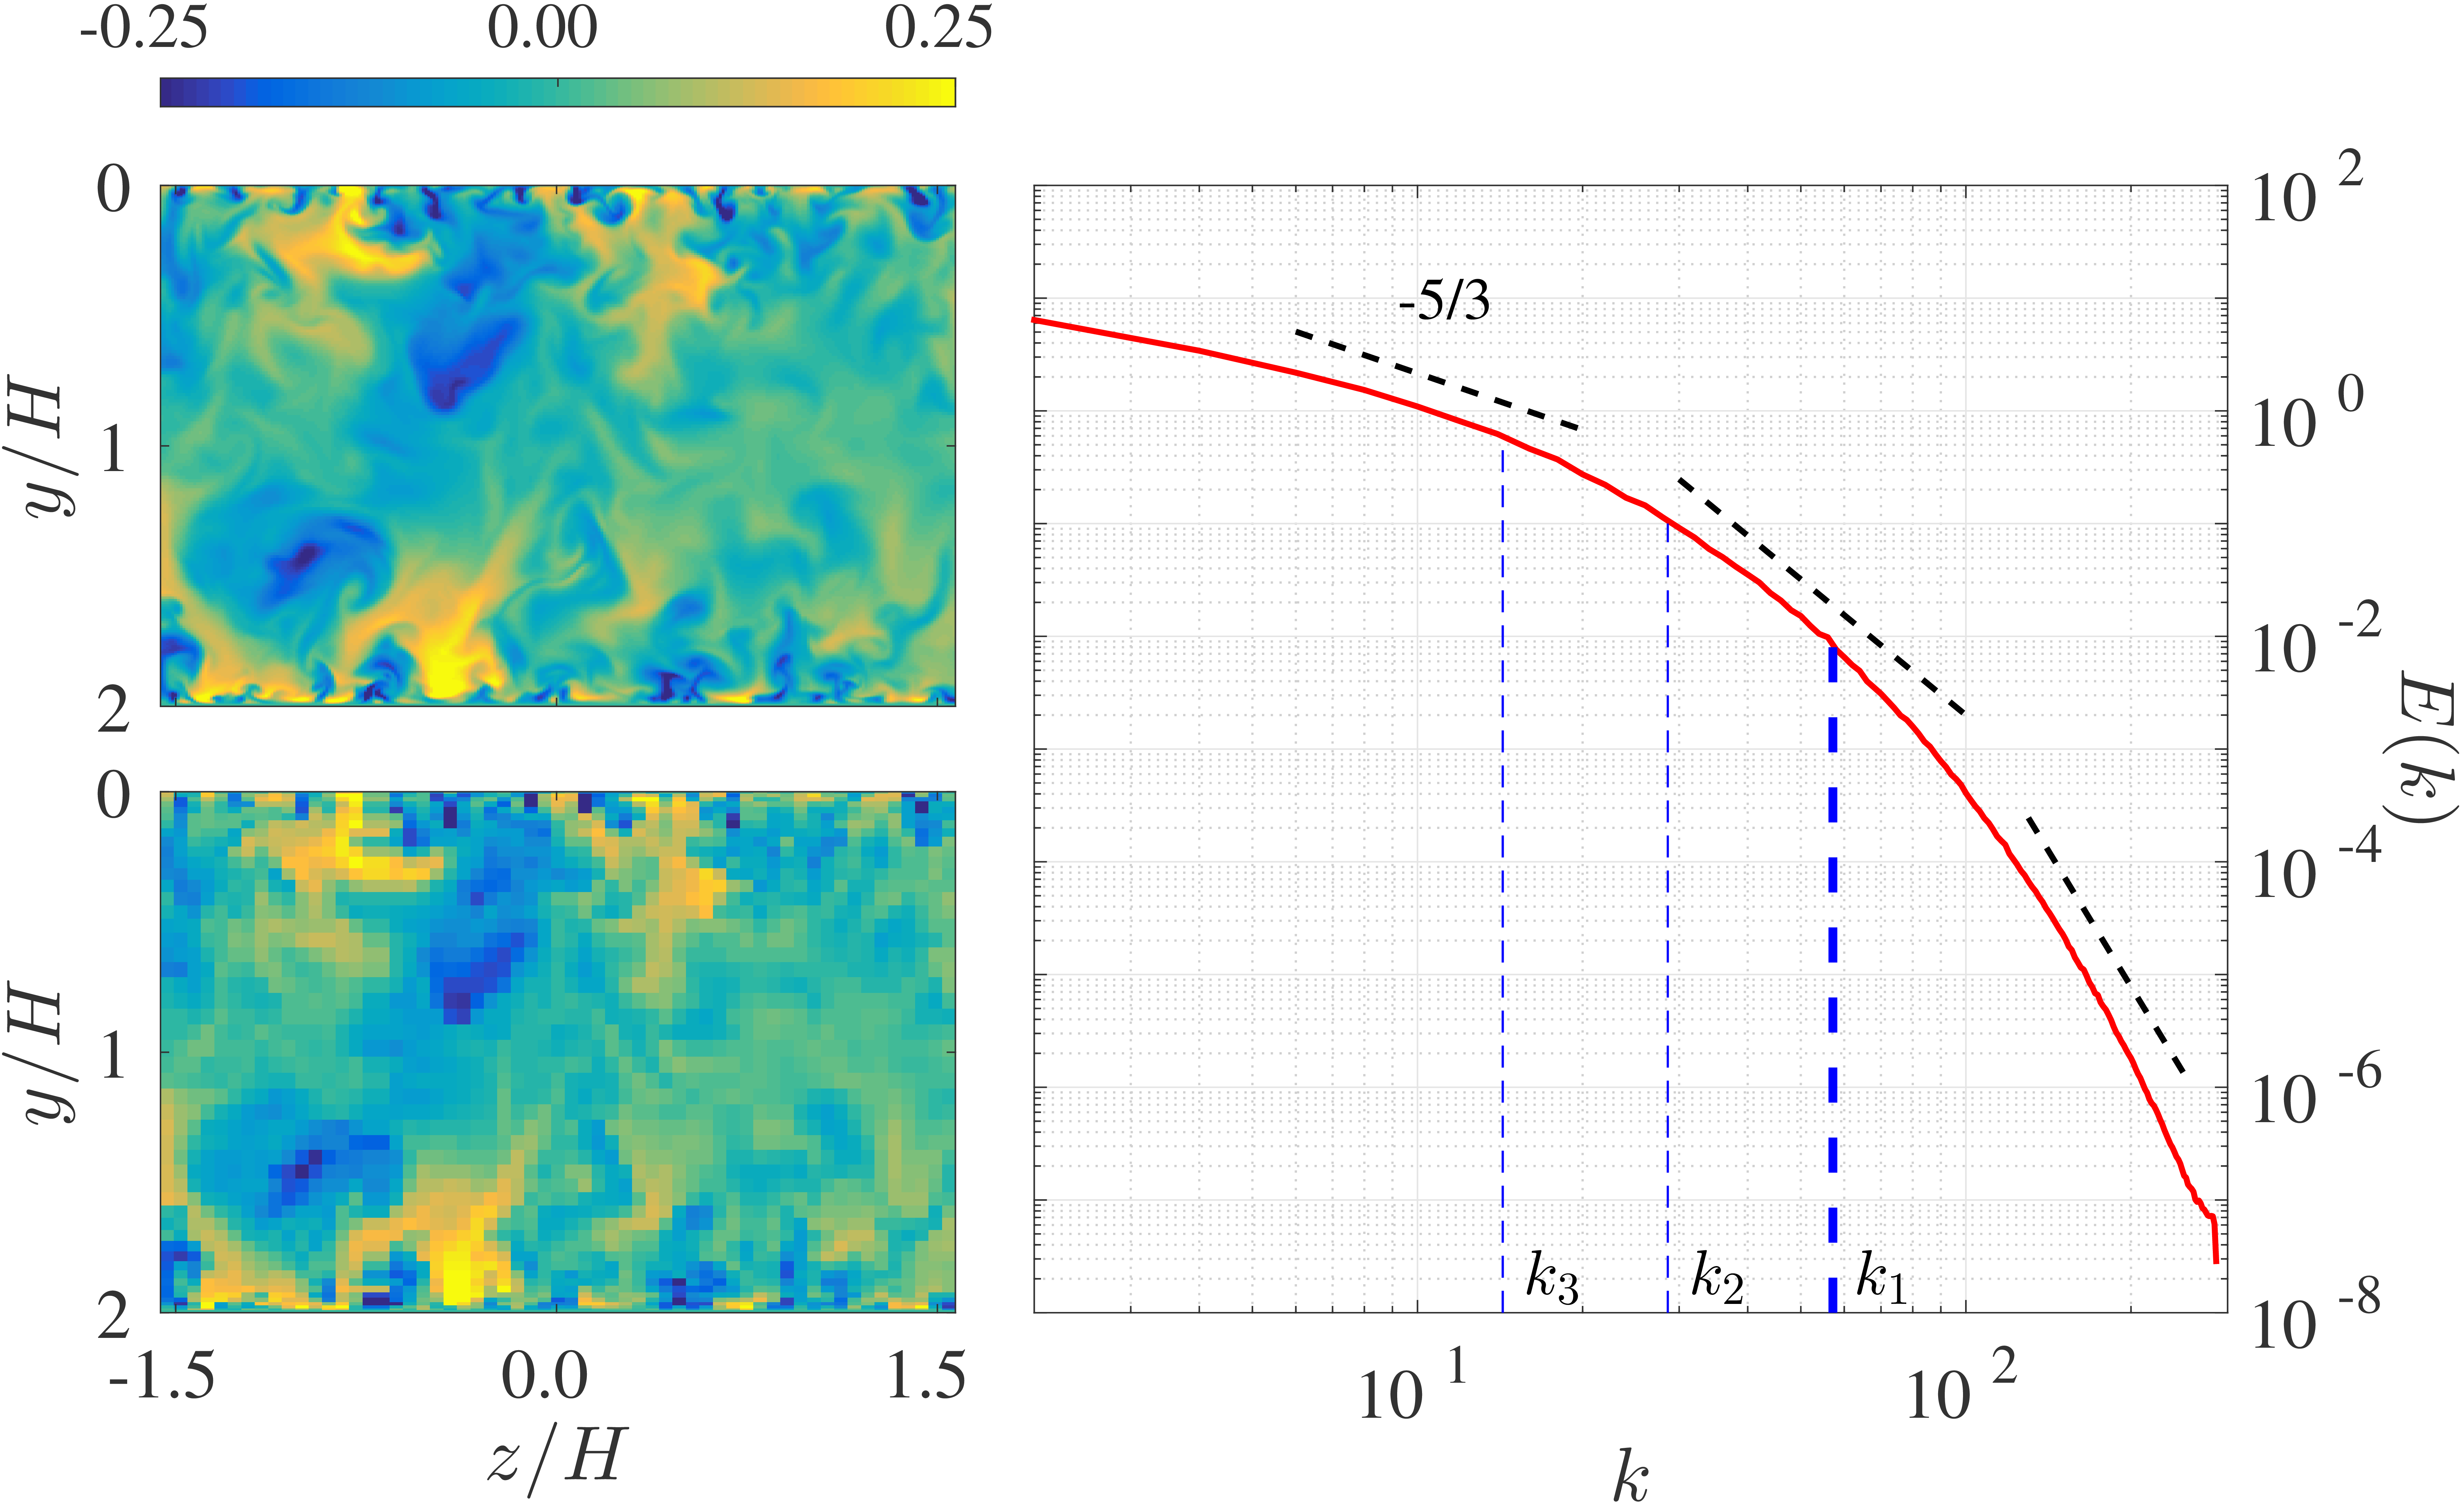
\includegraphics[width=0.85\textwidth]{./figures/turbulence/channel/samplevels_spectrum_spanwise_refDNS_kc1.png}}
			\caption*{Subsample by $ 5 \times 5 $ ($ k_1 $)}
			\onslide<3>	
			\centerline{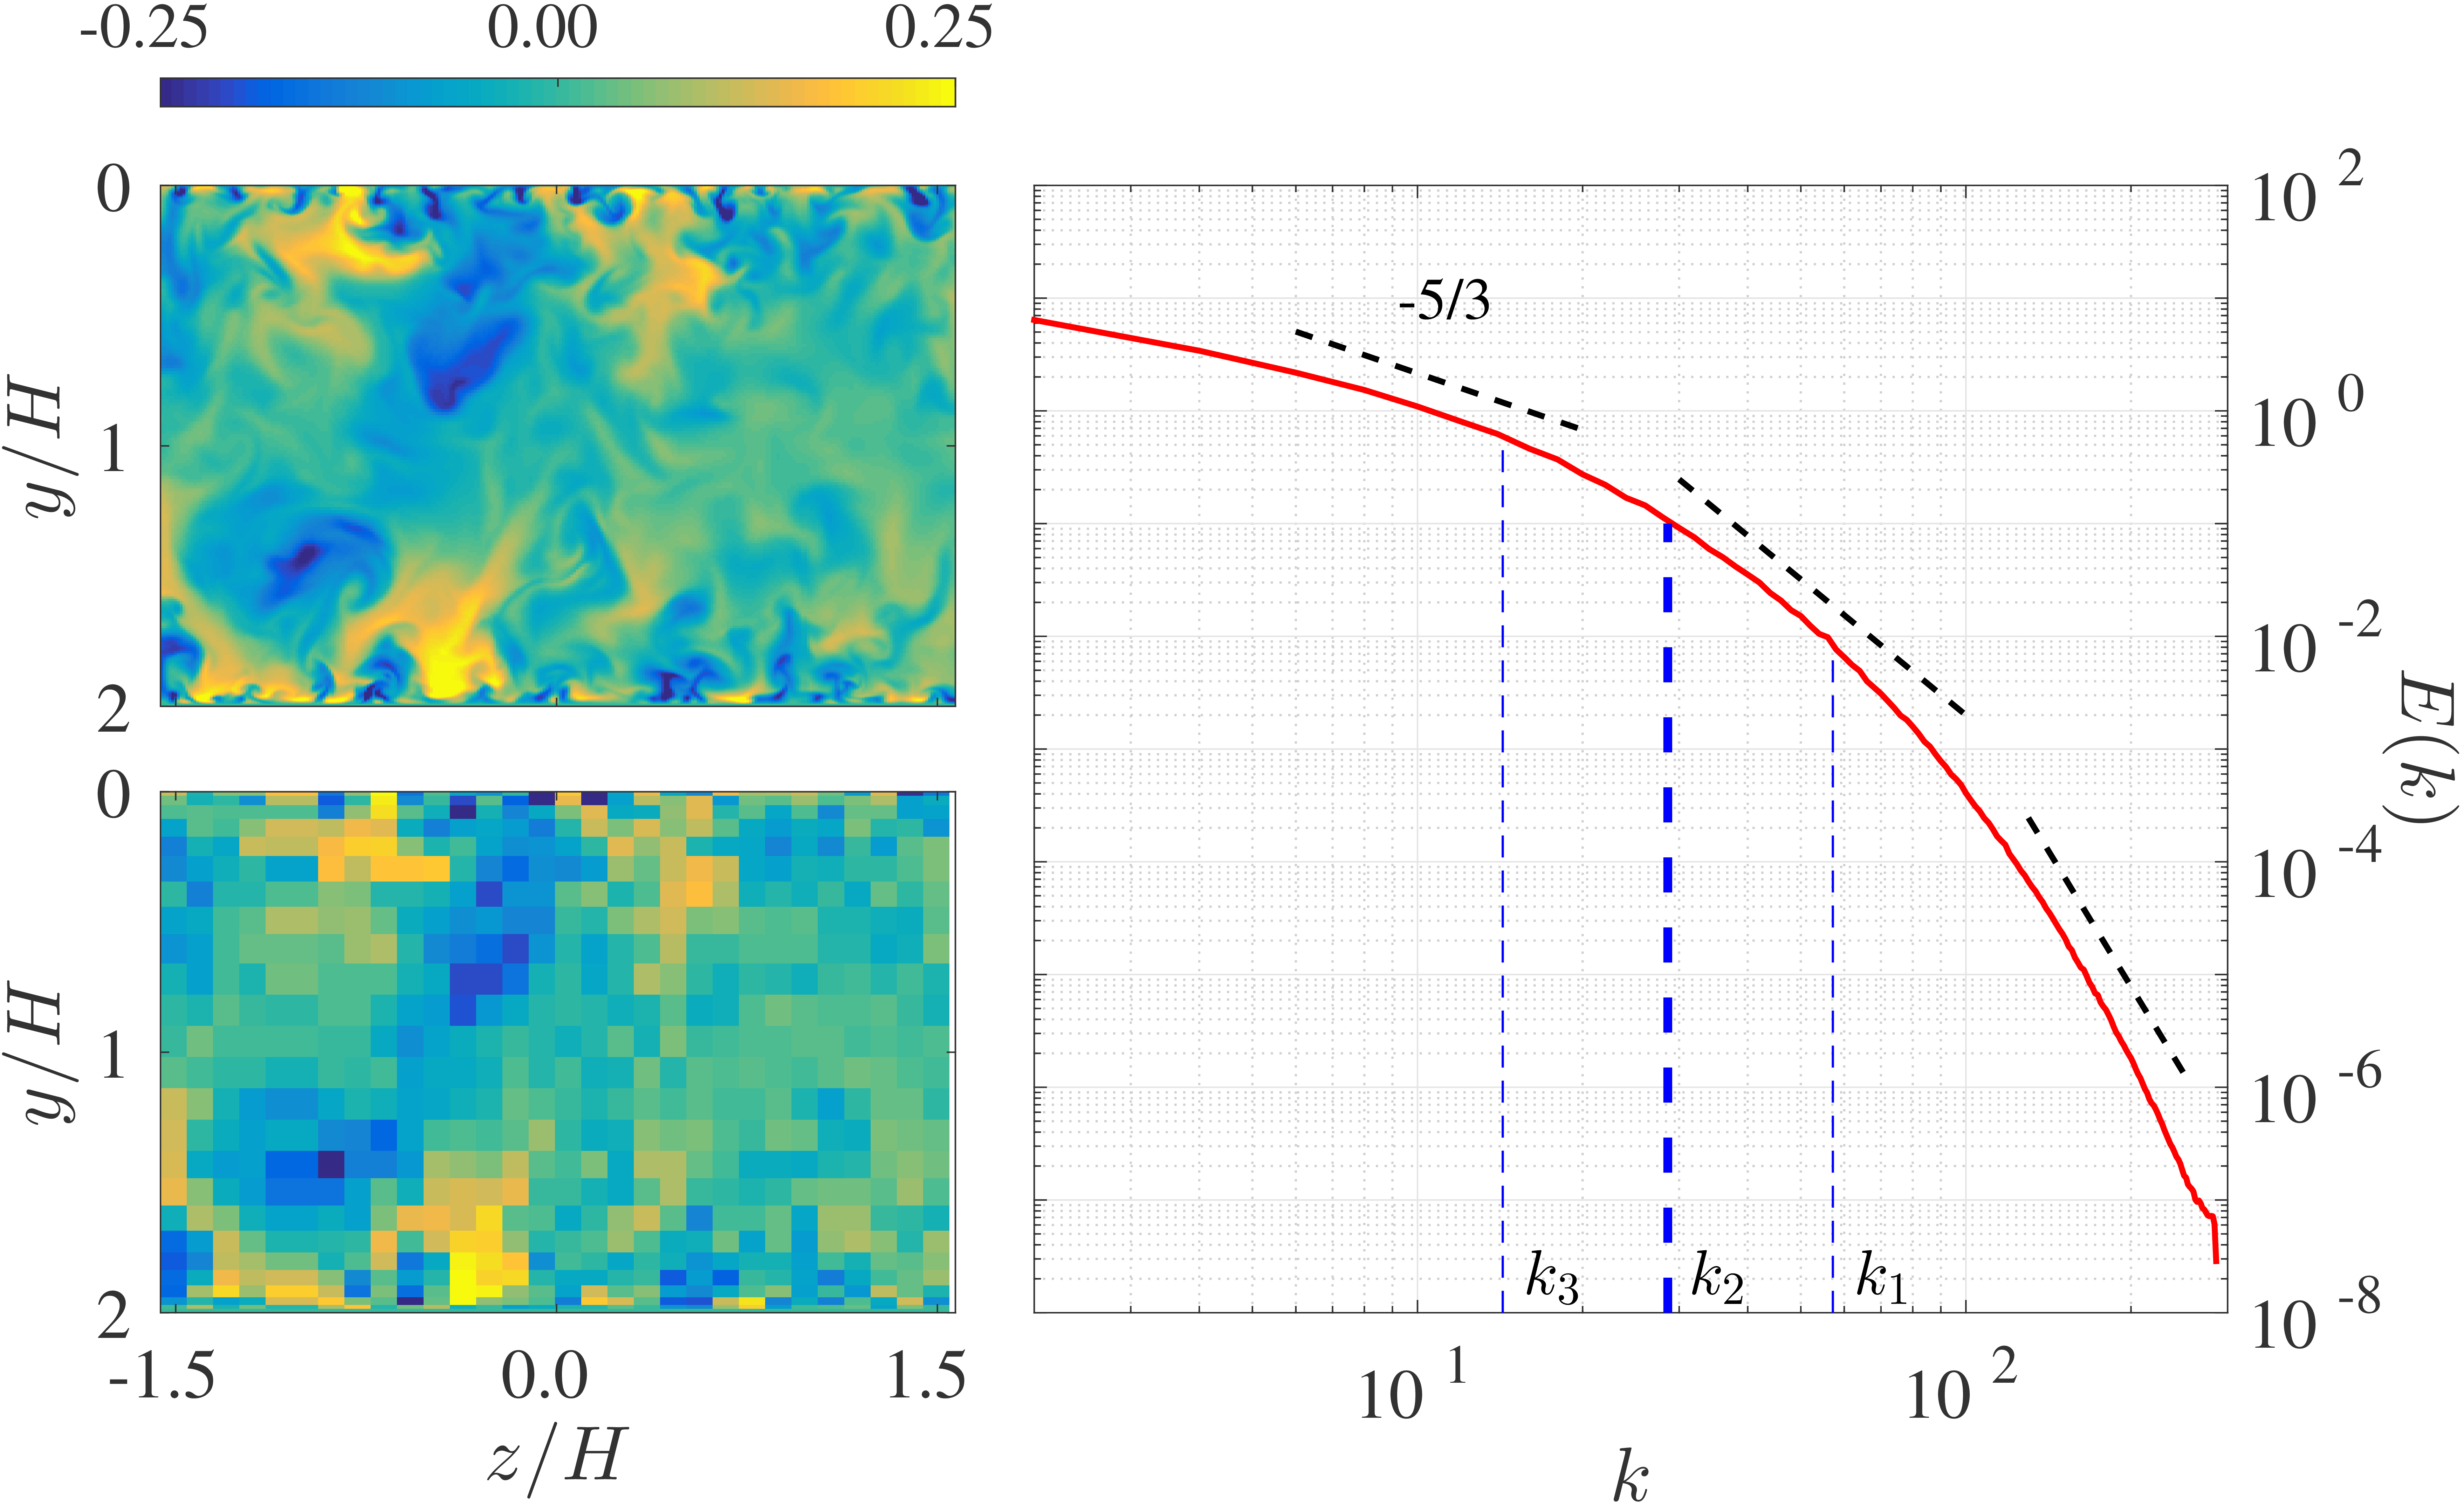
\includegraphics[width=0.85\textwidth]{./figures/turbulence/channel/samplevels_spectrum_spanwise_refDNS_kc2.png}}
			\caption*{Subsample by $ 10 \times 10 $ ($ k_2 $)}
			\onslide<4>	
			\centerline{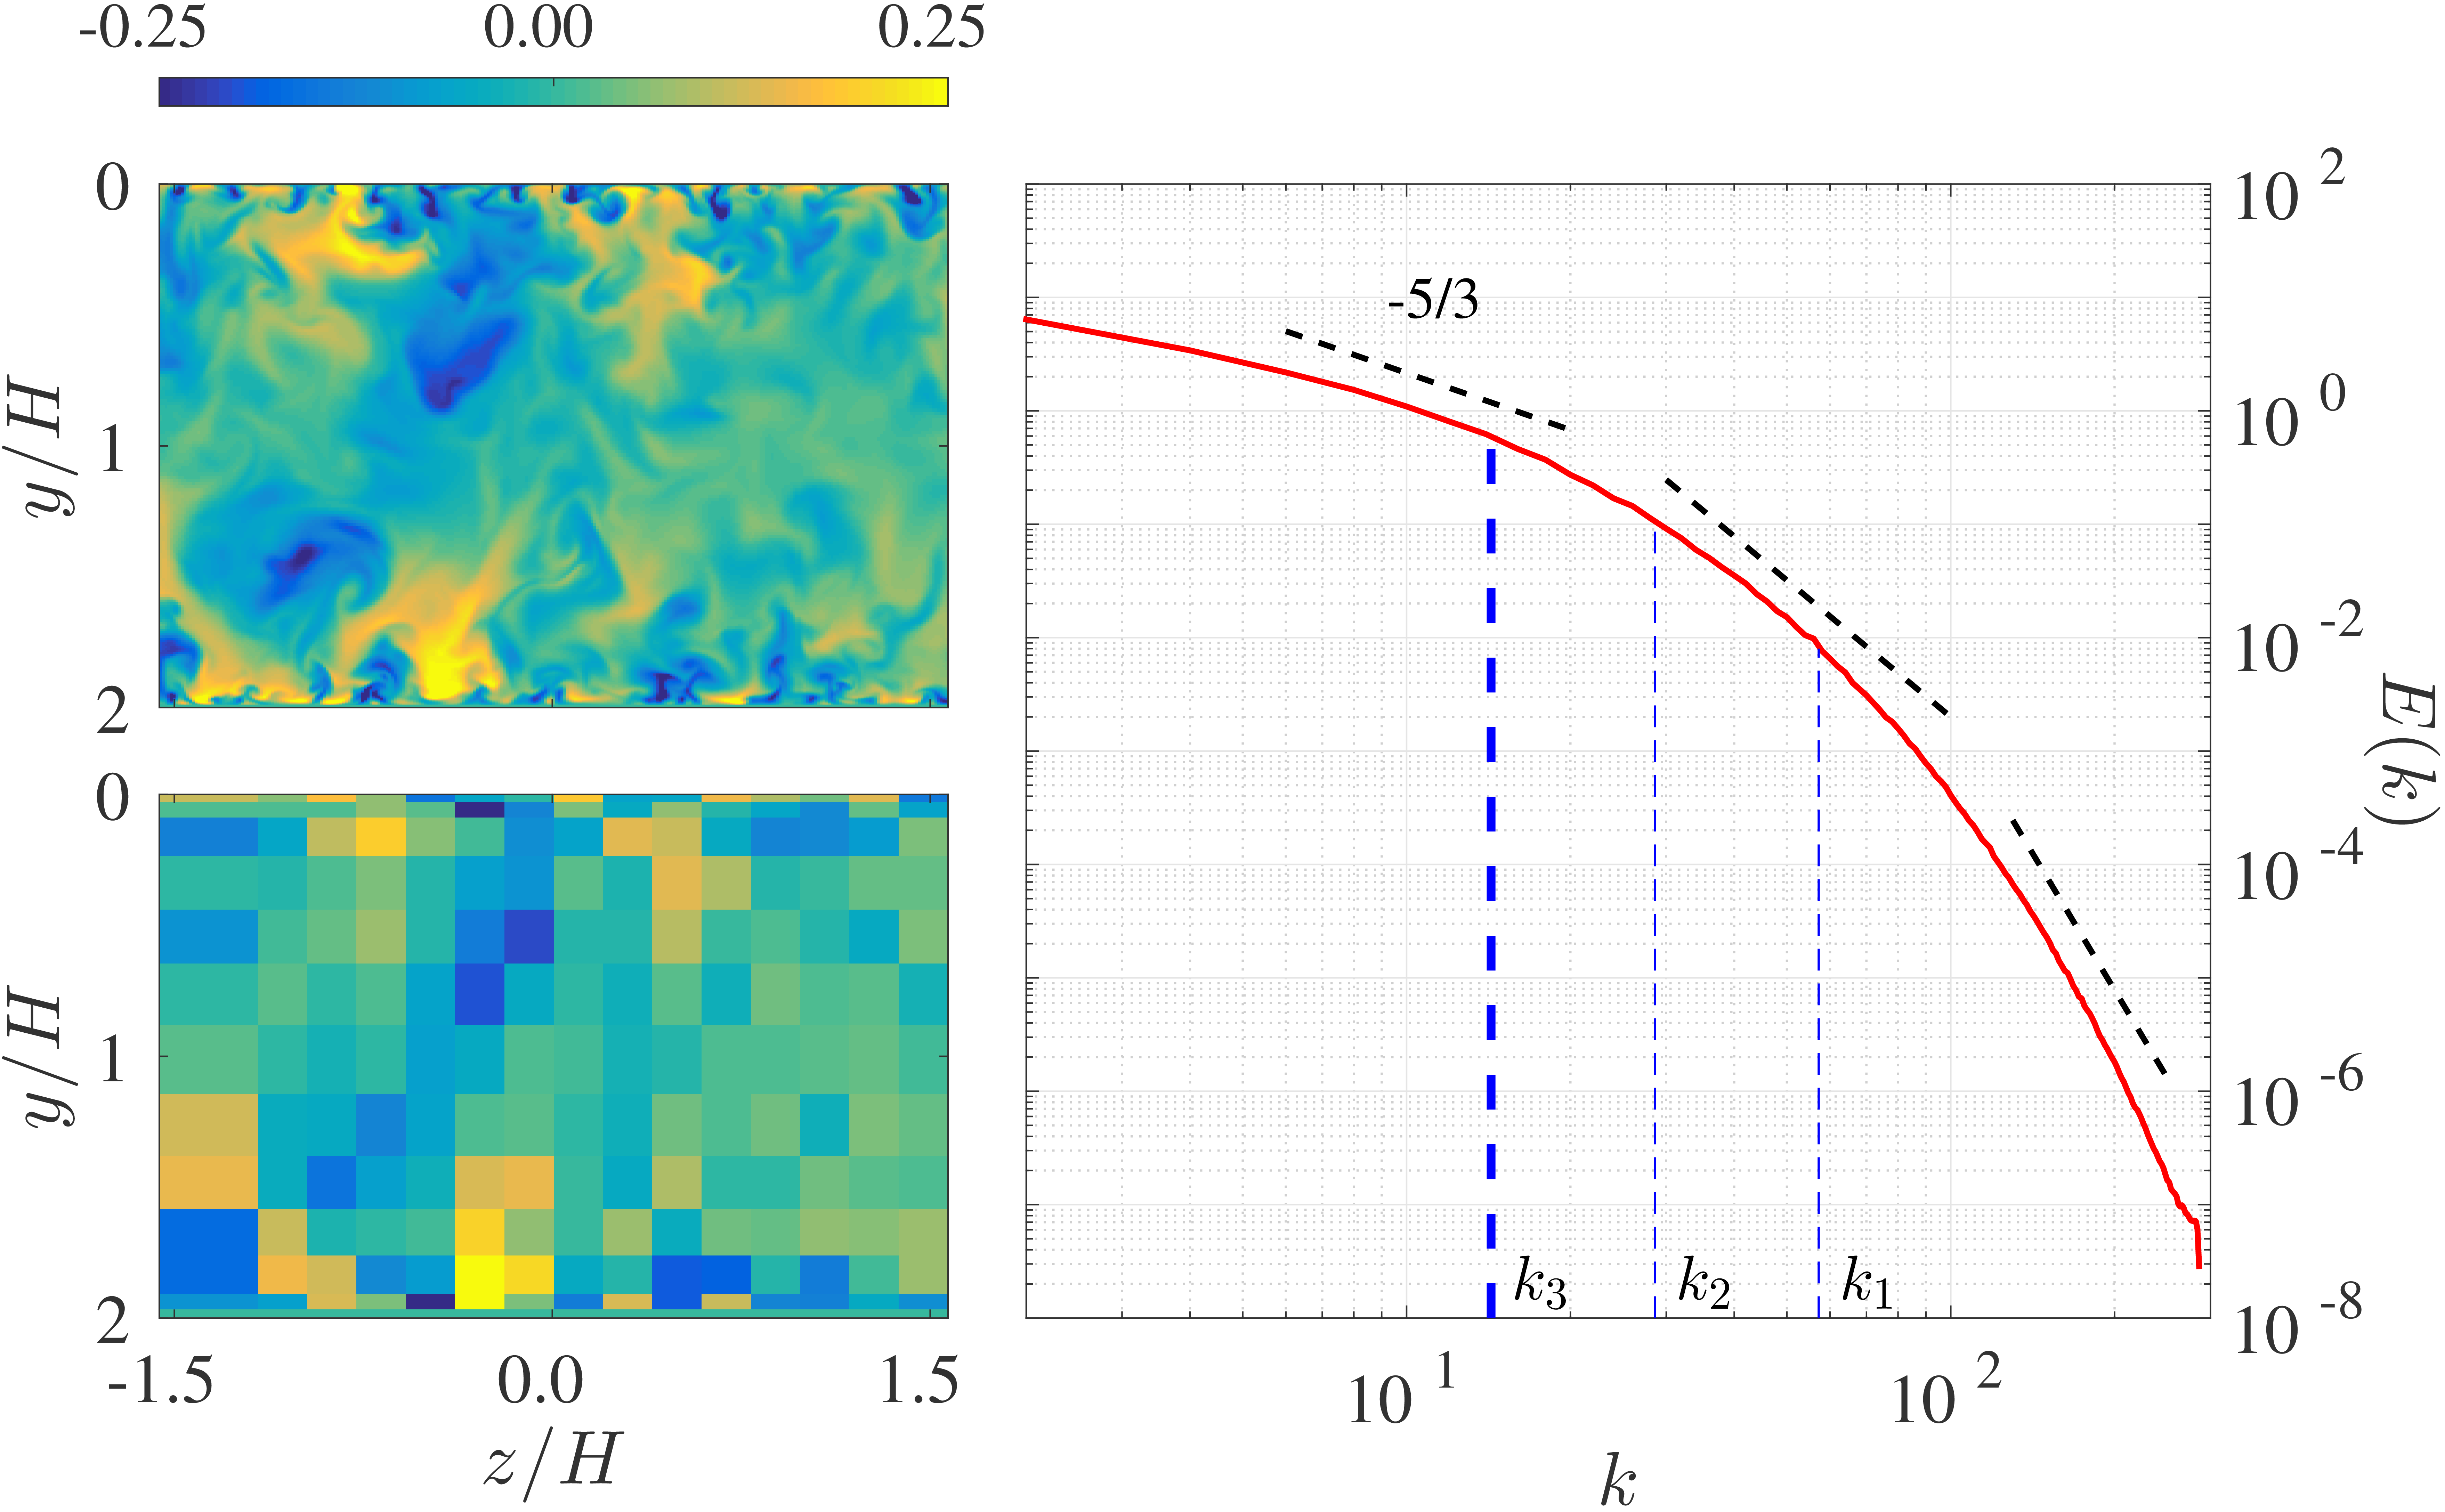
\includegraphics[width=0.85\textwidth]{./figures/turbulence/channel/samplevels_spectrum_spanwise_refDNS_kc3.png}}
			\caption*{Subsample by $ 20 \times 20 $ ($ k_3 $)}
		\end{overprint}				
	\end{figure} 		
\end{frame}

\begin{frame}
\frametitle{Problem 1: mapping functions between small \& large scales}

	\begin{figure}
		\begin{overprint}
			\onslide<1>	
			\centerline{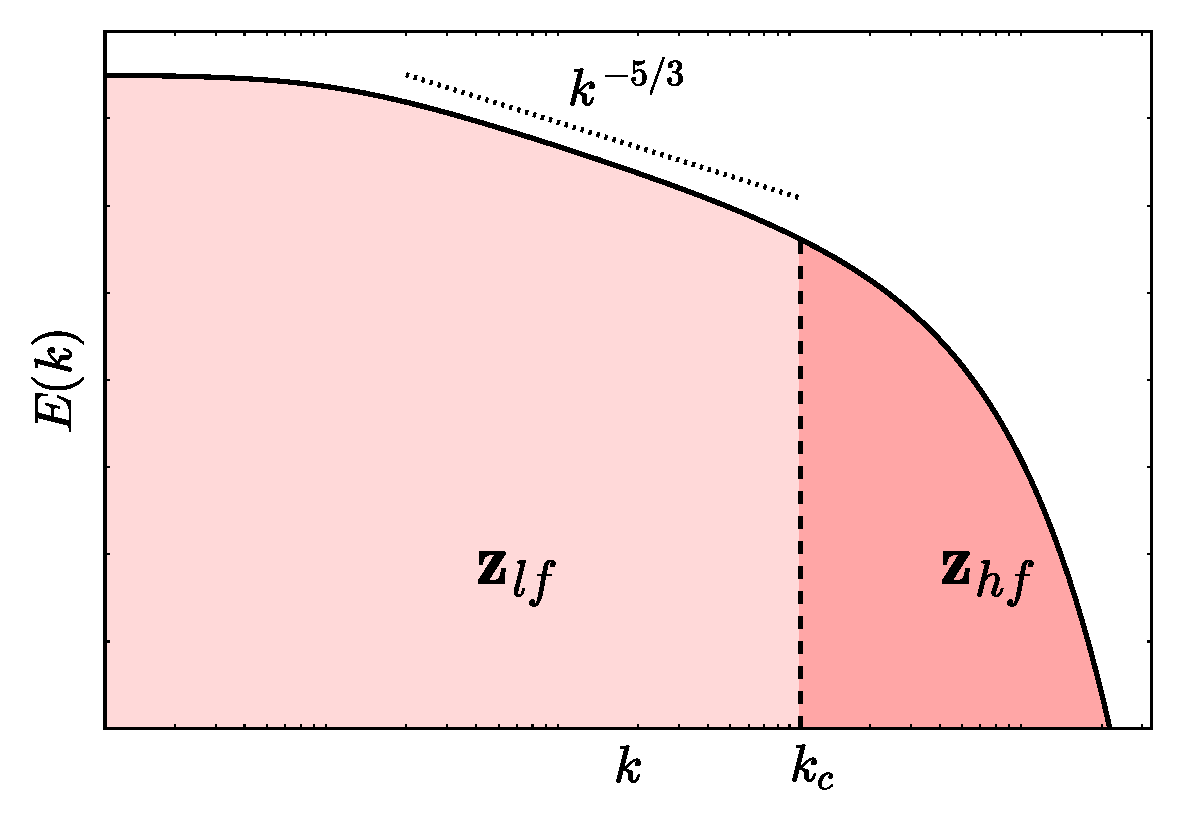
\includegraphics[width=0.75\textwidth]{./figures/turbulence/turbulence_spectra_long}}
			\onslide<2>	
			\centerline{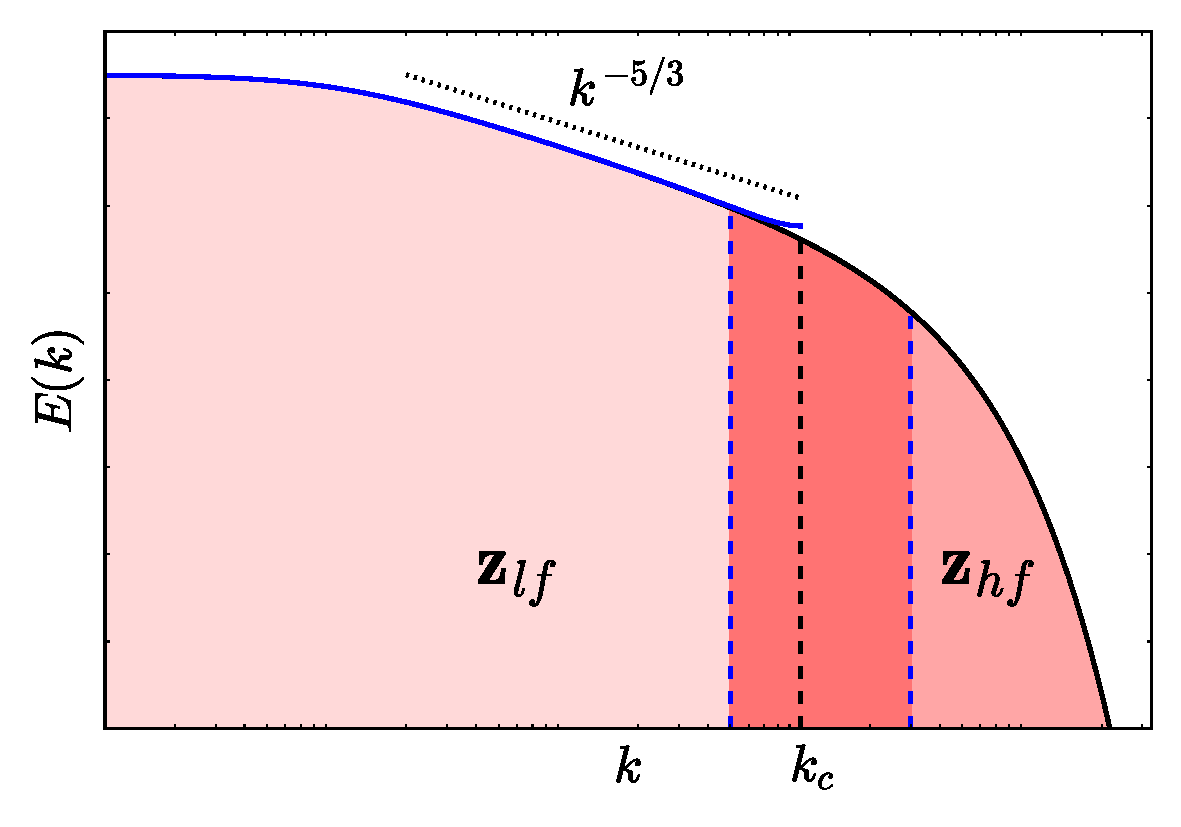
\includegraphics[width=0.75\textwidth]{./figures/turbulence/turbulence_spectra_long_alias}}			
		\end{overprint}	
	\end{figure}
\end{frame}

\begin{frame}
\frametitle{Problem 2: fusion of complementary measurements}
	\begin{figure}
		\begin{overprint}
			\onslide<1>	
			\centerline{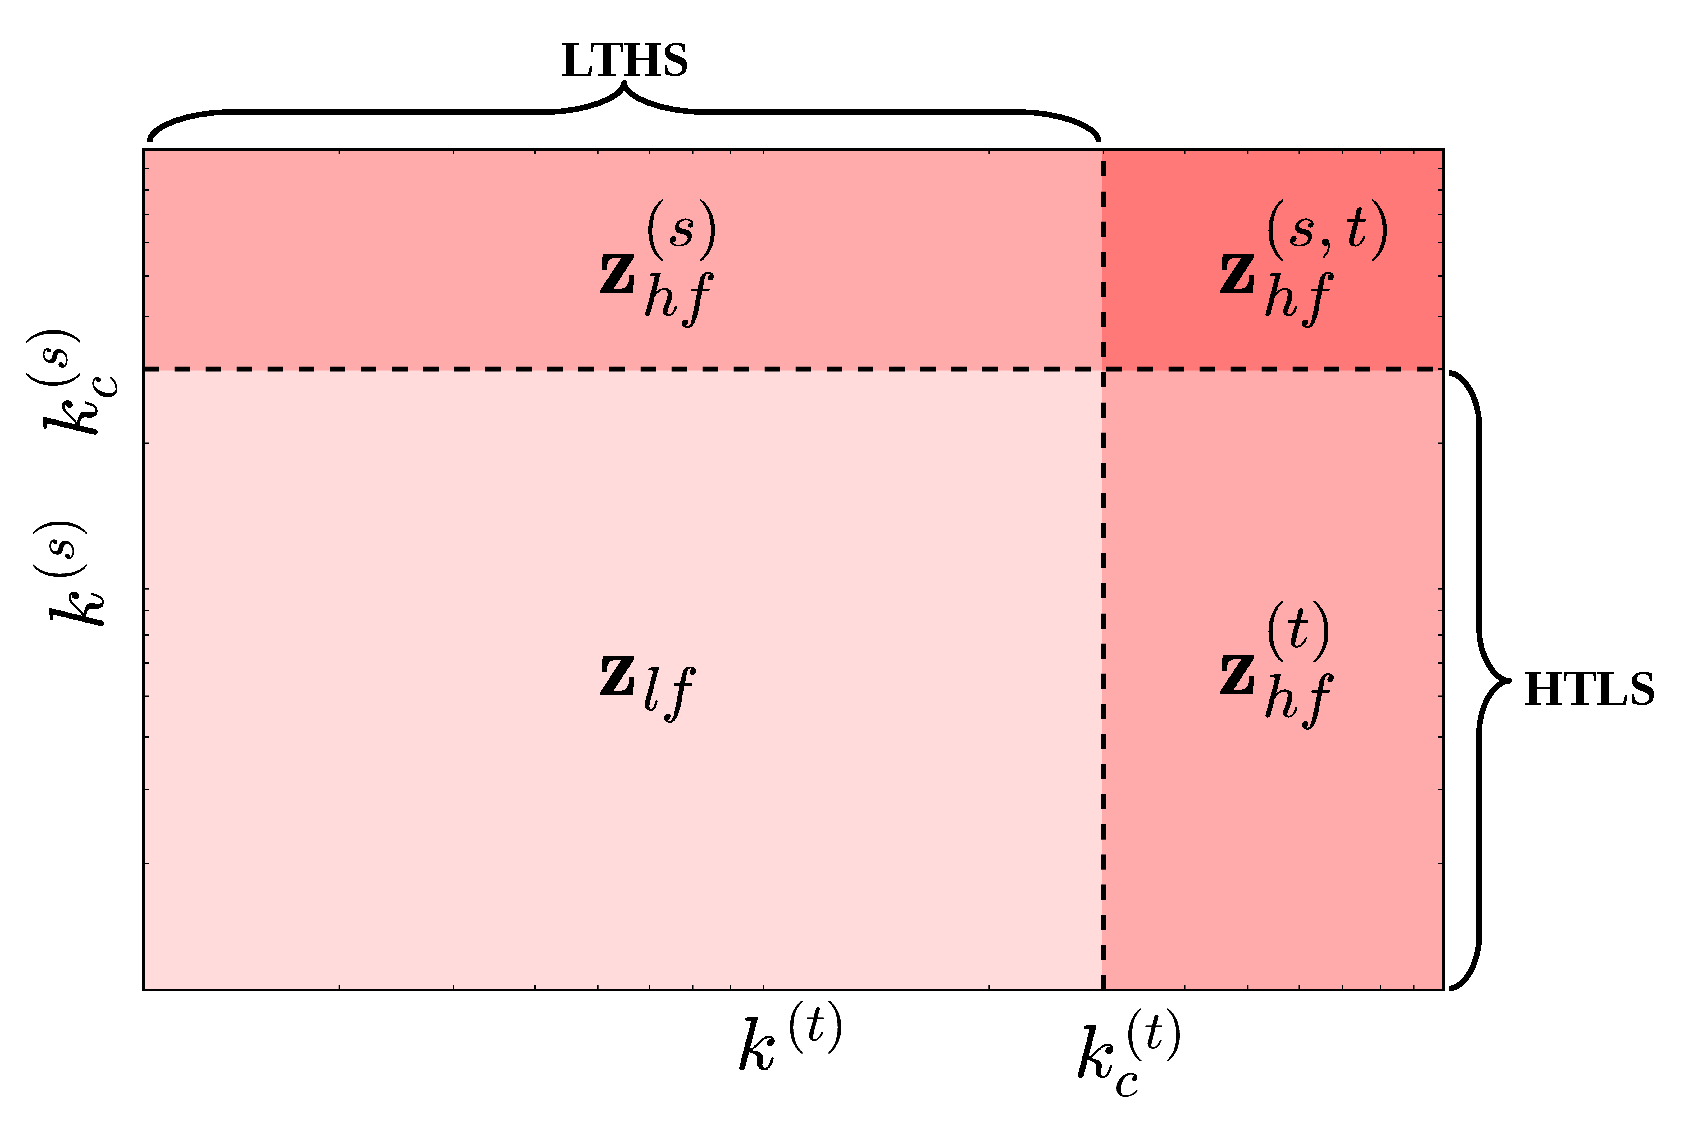
\includegraphics[width=0.85\textwidth]{./figures/turbulence/space_time_wavedomain_long.pdf}}
			\onslide<2>
			\centerline{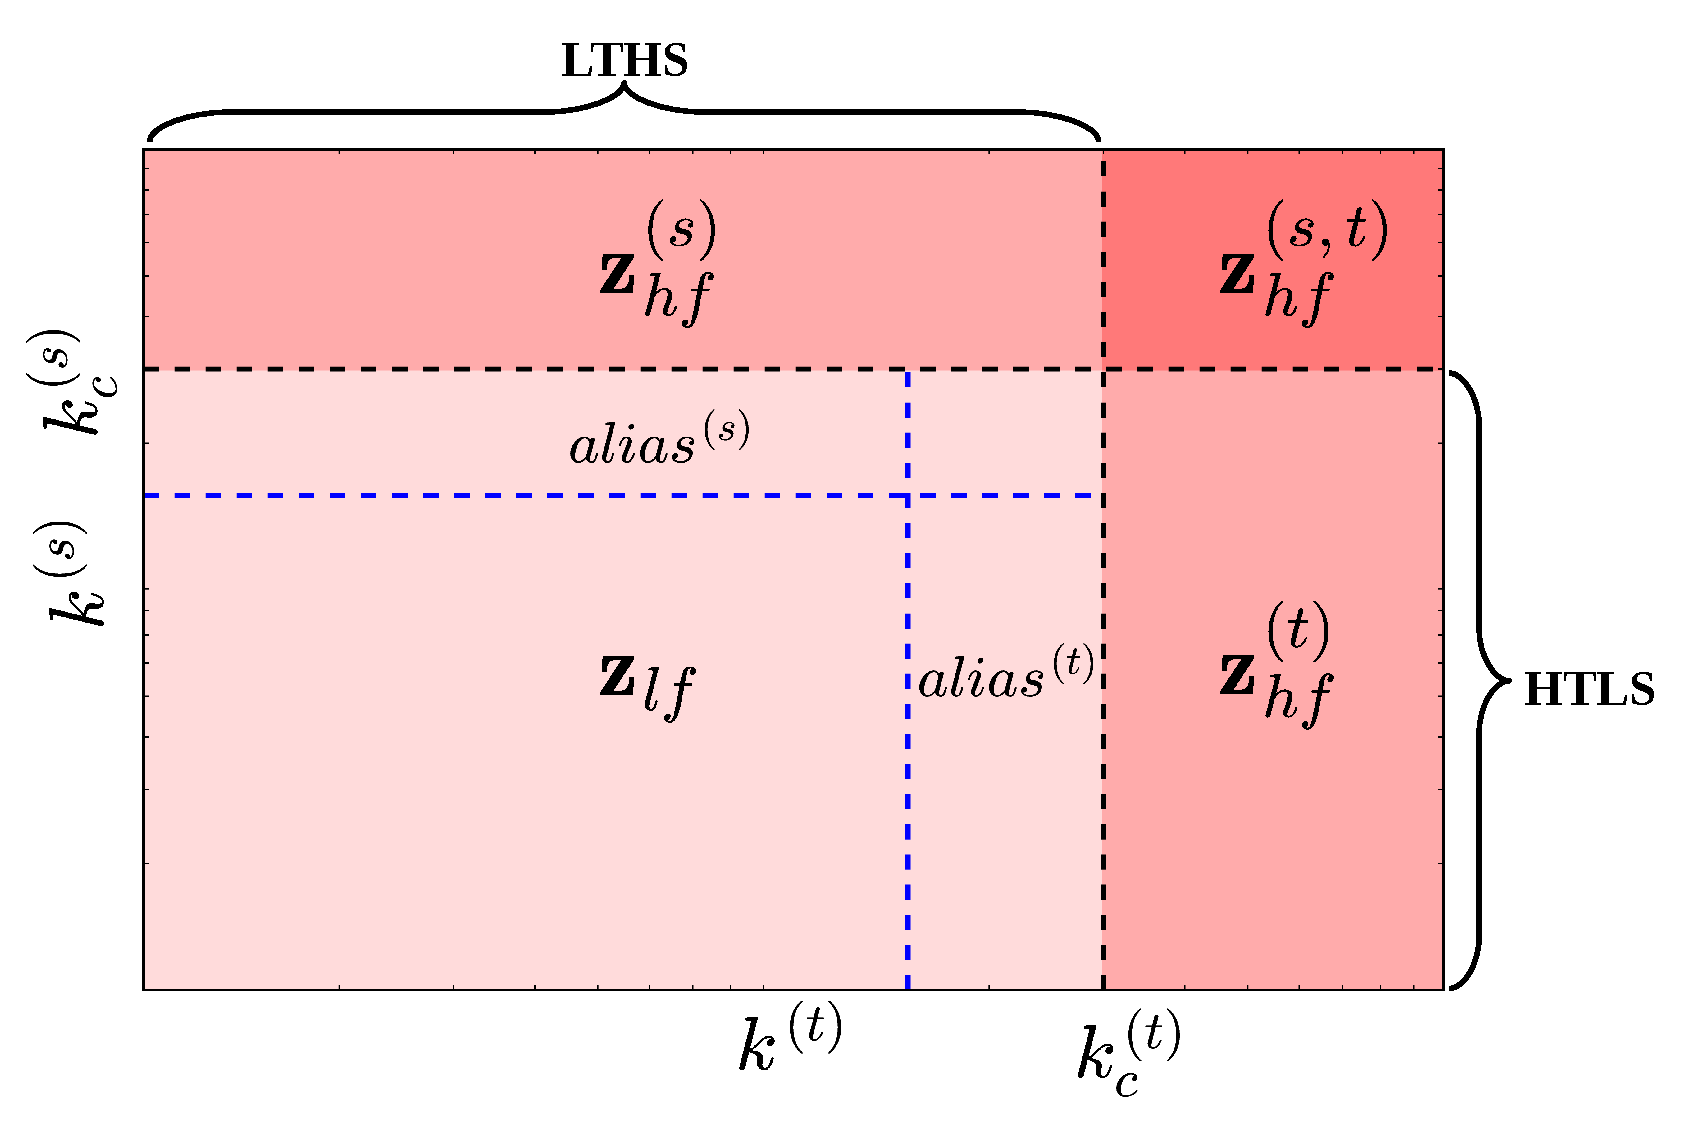
\includegraphics[width=0.85\textwidth]{./figures/turbulence/space_time_wavedomain_long_alias.pdf}}
		\end{overprint}			
	\end{figure}
\end{frame}

\subsection[Datasets]{Datasets for numerical experiments}
\begin{frame}
\frametitle{Numerical datasets}
	\begin{overprint}
		\onslide<1>
		Two numerical datasets of full resolution are used:
		\begin{enumerate}[(i. )]
			\item \textbf{\color{red} Isotropic turbulence}: 37 blocks of 3D field of $ 96^3 $ ($ Re_\lambda = 90$, $ 384^3 $) \\
			\item {\color{black!20} \textbf{\color{red!20} Turbulent channel flow}: 10000 snapshots of $ 257 \times 288 $, $ Re_\tau = 550 $}
		\end{enumerate}
		\begin{figure}
			\centering
			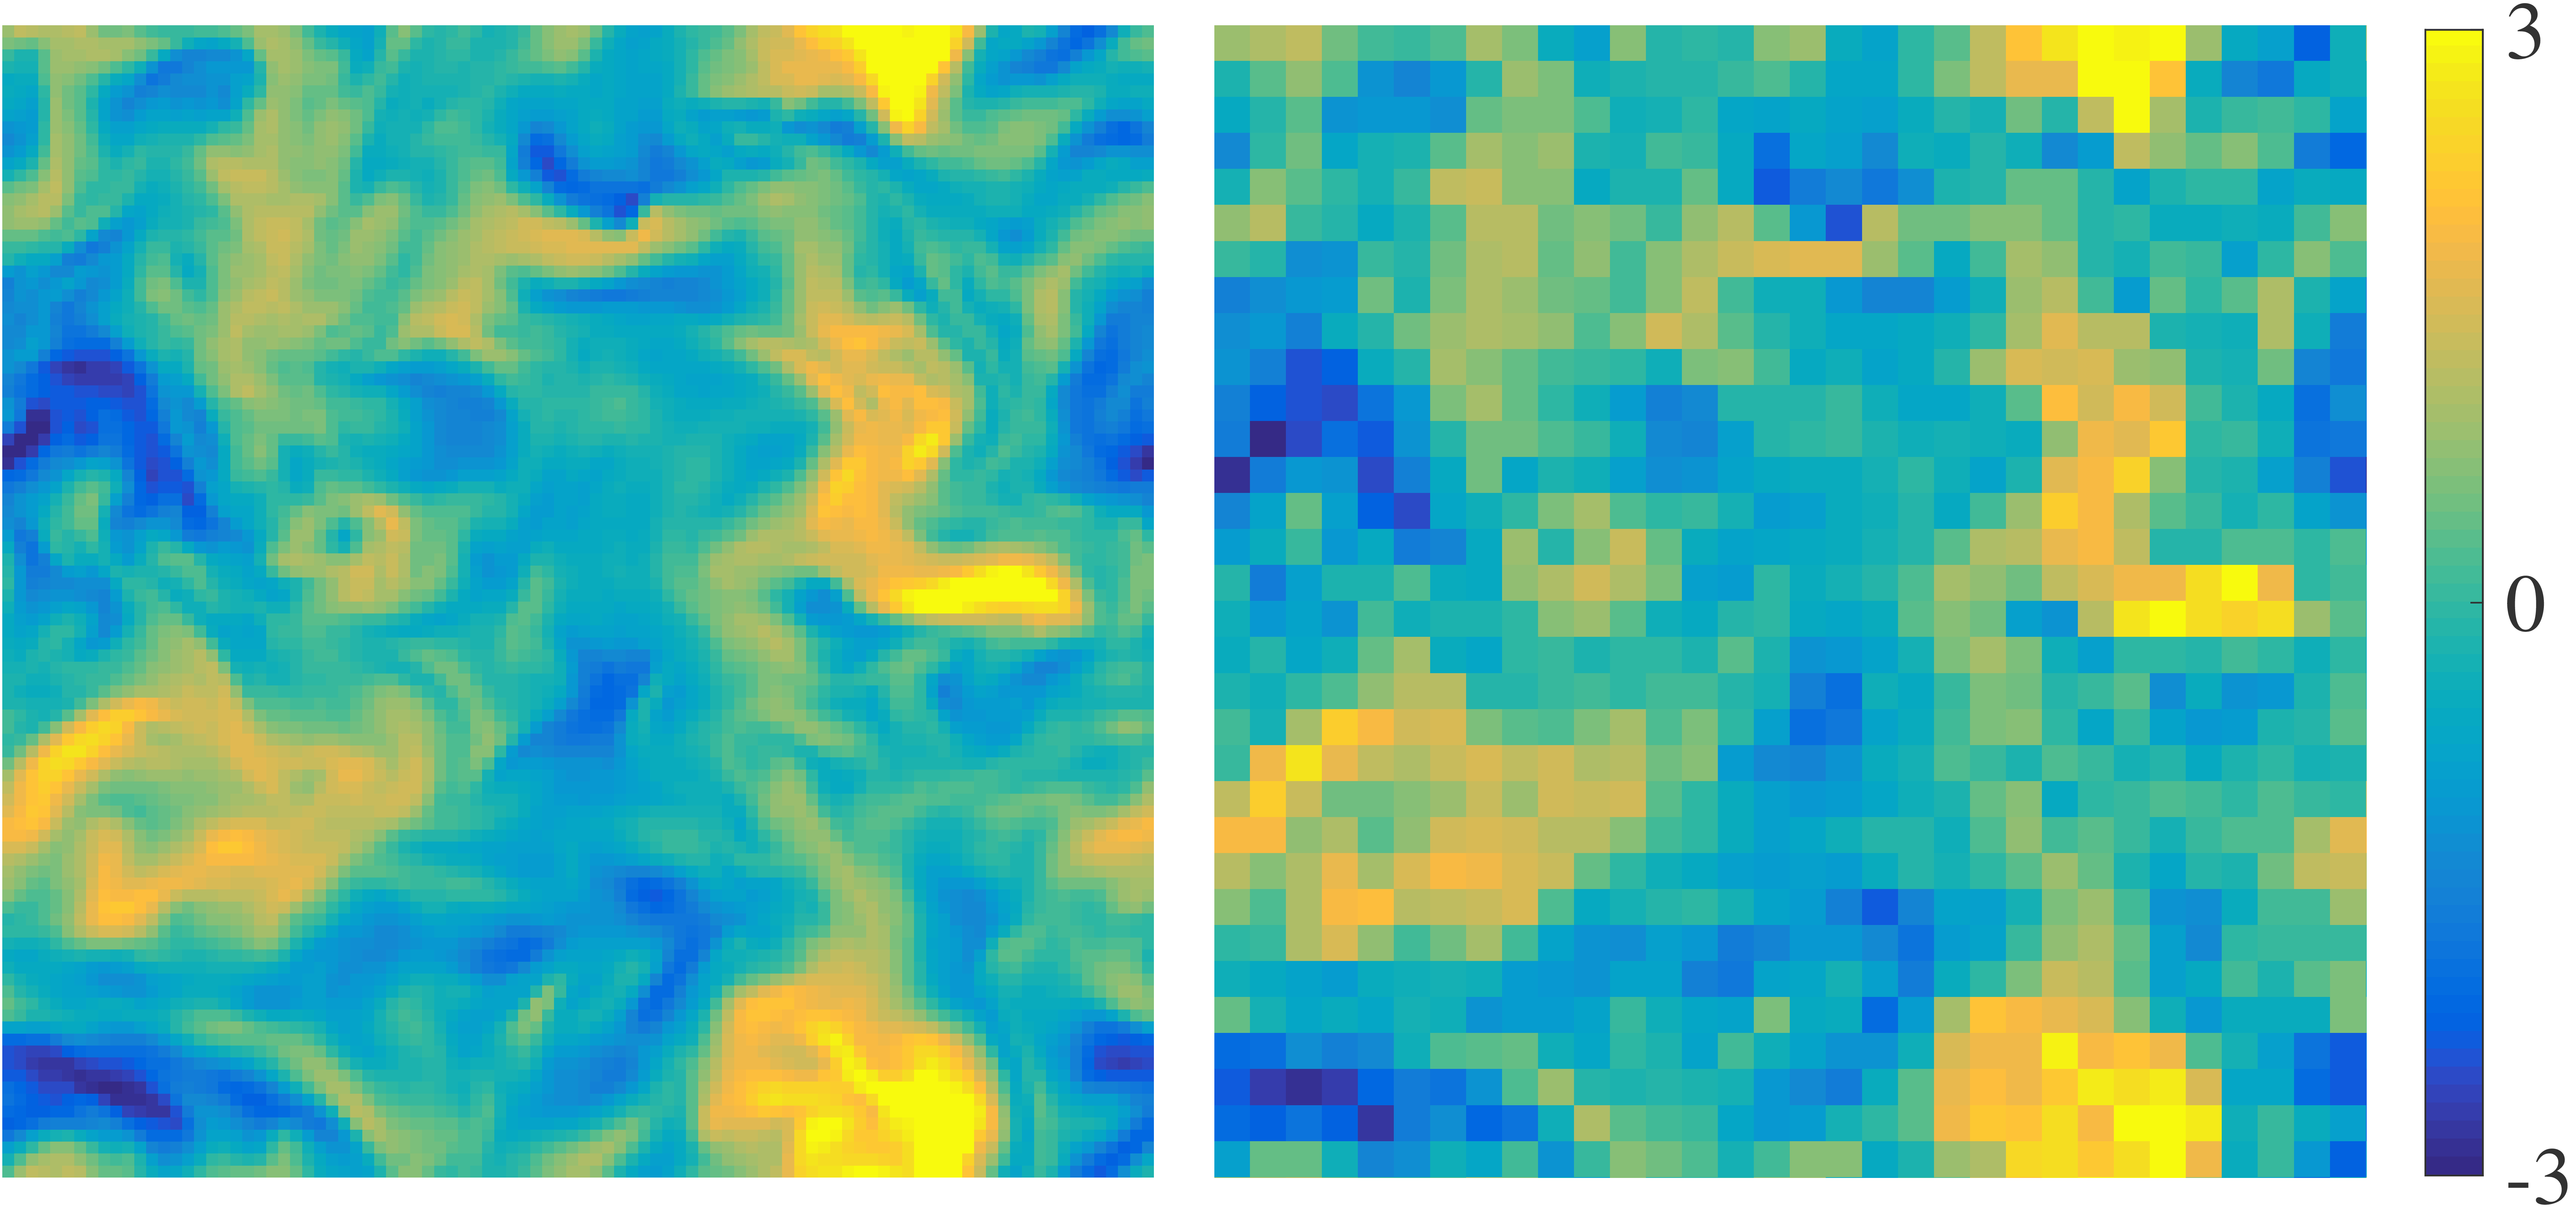
\includegraphics[height=4.2cm]{./figures/turbulence/isotropic/u_HR_2D.png}
			\caption*{Sample streamwise velocity field of isotropic turbulence at $ Re_\lambda = 90$}
		\end{figure}		
	
		\onslide<2>
		Two numerical datasets of full resolution are used:
		\begin{enumerate}[(i. )]
			\item {\color{black!20} \textbf{\color{red!20} Isotropic turbulence}: 37 blocks of 3D field of $ 96^3 $ ($ Re_\lambda = 90$, $ 384^3 $)} \\
			\item \textbf{\color{red} Turbulent channel flow}: 10000 snapshots of $ 257 \times 288 $, $ Re_\tau = 550 $
		\end{enumerate}
		\begin{figure}
			\centering
			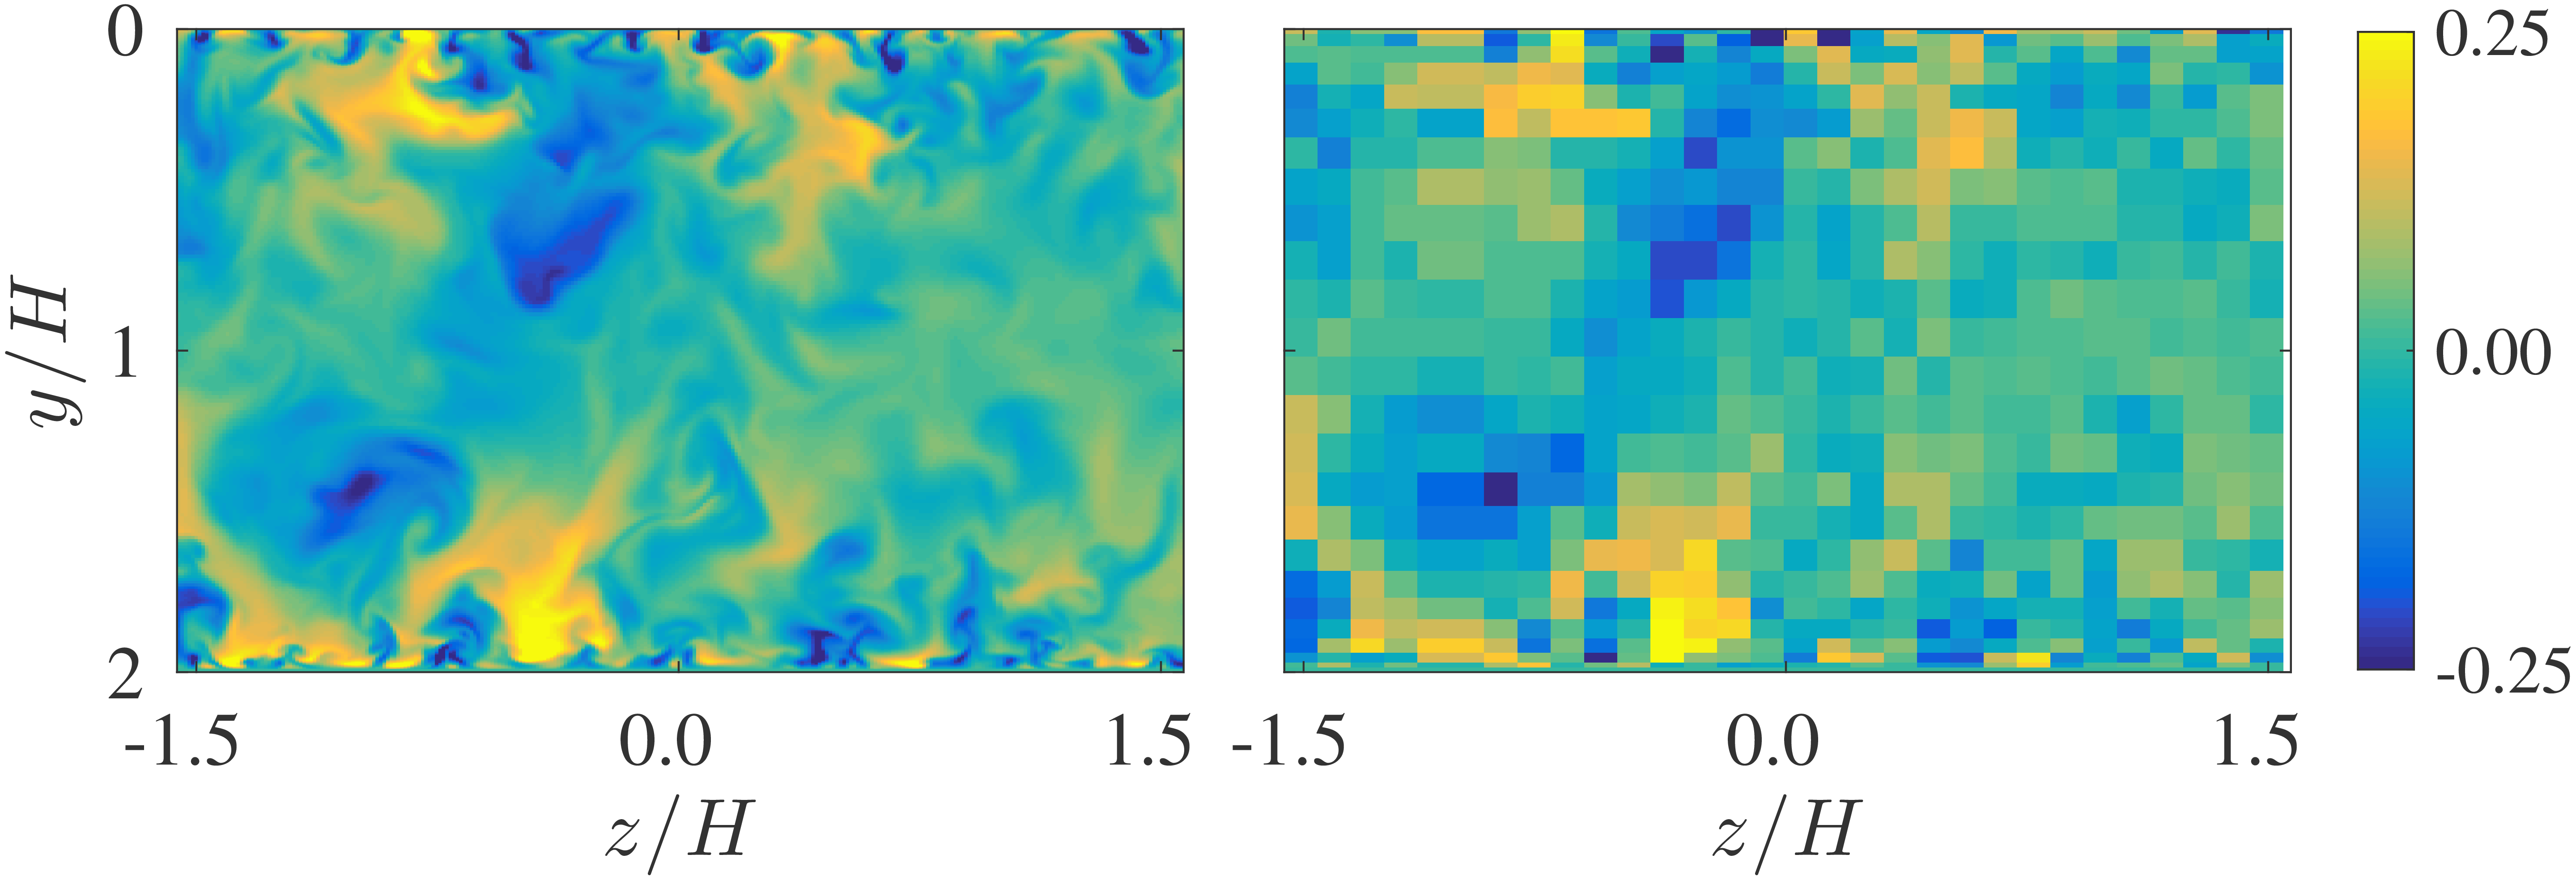
\includegraphics[height=4.2cm]{./figures/turbulence/channel/samplesnap_2D.png}
			\caption*{Sample streamwise velocity field of the channel flow at $ Re_\tau = 550$}
		\end{figure}		
	\end{overprint}
\end{frame}

% % % % % % % % % % % % % % % % % % % % % % % % % % % % % % % % % % % % % % % % % % % % % %
% % % % % % % % % % % % % % % % % % % % % % % % % % % % % % % % % % % % % % % % % % % % % %
% % % % % % % % % % % % % % % % % % % % % % % % % % % % % % % % % % % % % % % % % % % % % % 

\section[Approaches]{The proposed approaches}
\subsection[Related approaches]{Related approaches}
\begin{frame}
\frametitle{Approaches in the literature}
	\begin{block}{\textbf{Reconstruction methods in turbulence studies}:}
		\begin{itemize}
			\item \textbf{Least-square} regression {\footnotesize \cite{durgesh2010multi}}
			\item \textbf{POD} reduced-order model {\footnotesize \cite{bonnet1994stochastic}}
			\item \textbf{Data assimilation} using Kalman filter {\footnotesize \cite{papadakis2010data,tu2013integration}}
			\item \textbf{Physical priors}: div-curl regularization {\footnotesize\cite{corpetti2002dense}}, vortex-in-cell {\footnotesize \cite{schneiders2014time}}
		\end{itemize}
	\end{block}
	\vfill
	\pause
	\begin{figure}
		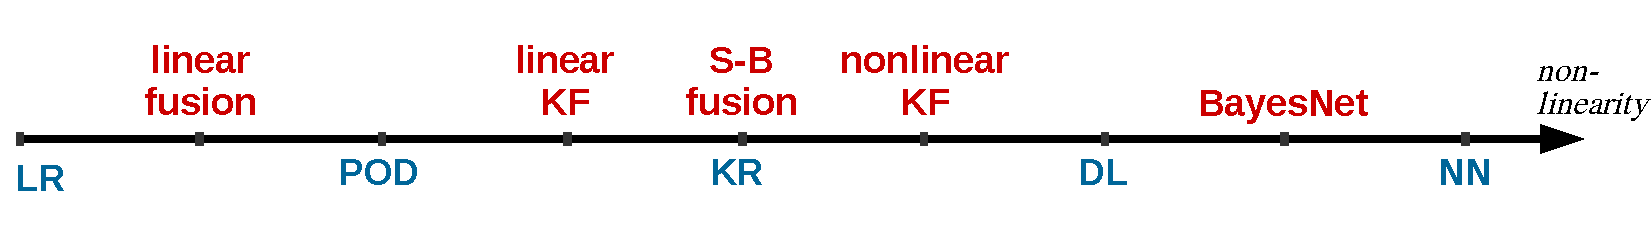
\includegraphics[width=\textwidth]{./figures/turbulence/models_spectrum.pdf}
	\end{figure}	
			
\end{frame}

\begin{frame}
\frametitle{Approaches in the present work}	
	\begin{block}{\textbf{Approach 1: learn a mapping function between scales}}
	\textbf{Objective}: $ \z_\ell \in {\rm I\!R}^\dimsl \mapsto  \z_h \in {\rm I\!R}^\dimsh $, $ \dimsh \gg \dimsl$ 
		\begin{itemize}
			\item \textbf{\color{red} Regression}: as set of coefficients\\
			\item \textbf{\color{red} Coupled dictionary learning}: coupled representations of LR/HR\\
		\end{itemize}
	\end{block}
	\vfill
	\begin{block}{\textbf{Approach 2: fusion of complementary measurements}}
	\textbf{Objective}: find $ \z$ given two measurements $ \x$ and $ \y$
		\begin{itemize}
			\item \textbf{\color{red} Non-local means}: self similarity of flow structures\\
			\item \textbf{\color{red} Bayesian fusion}: \textit{maximum a posteriori} estimate $p \left(\z|\x,\y\right)$	
		\end{itemize}
	\end{block}	
\end{frame}


% % % % % % % % % % % % % % % % % % % % % % % % % % % % % % % % % % % % % % % % % % % % % %
\subsection{Mapping functions between large and small scales}

\begin{frame}
\frametitle{Regression}	
	\begin{tcolorbox}[colback=red!5!white,colframe=red!75!black]	
		Learn $ f $ from training samples $ \left(\y_t, \z_t\right) $: 
		\begin{equation*}
			f:  \y_t \mapsto  \hat{\z}_t = f(\y_t) + \n^{(t)} \approx B^{\mytrans}\y_t 
		\end{equation*}
 	\end{tcolorbox}	
 	\begin{itemize} \itemsep0em
 	\item Linear regression:
 	\begin{equation*}
	 	\B= \argmin_\B{ \{ \underbrace{\Vert \Y\B-\Z\Vert^2_2}_{\text{data misfit}} + \underbrace{\lambda g(\B)}_{\text{penalty}} \} }
 	\end{equation*}
	\begin{itemize}
		\item \textbf{\color{red}Ridge regression}: $ g(\B) = \Vert \B\Vert^2_2 $
		\item \textbf{\color{red}LASSO}: $ g(\B) = \Vert \B\Vert_1 $
	\end{itemize} 	
	
	\item Nonlinear regression: projection into kernel space (\textbf{\color{red}KRR})
	\item Parameter estimation: \emph{bias-variance} trade-off, \textit{k-fold} cross validation
	\end{itemize} 	
\end{frame}

\begin{frame}
	\frametitle{Dictionary learning: a generalization of POD} 
	\begin{itemize}
		\item Data representation: linear transformation via a ``\emph{dictionary}''
		\begin{equation*}
			\X  = \dict \dictco
		\end{equation*}

		\item Dictionary learning: $ \dict $ is \emph{redundant} (or \emph{overcomplete}), $ \dictco $ is \emph{sparse}
		\begin{figure}
		\centering
		\vspace*{-0.0cm}
		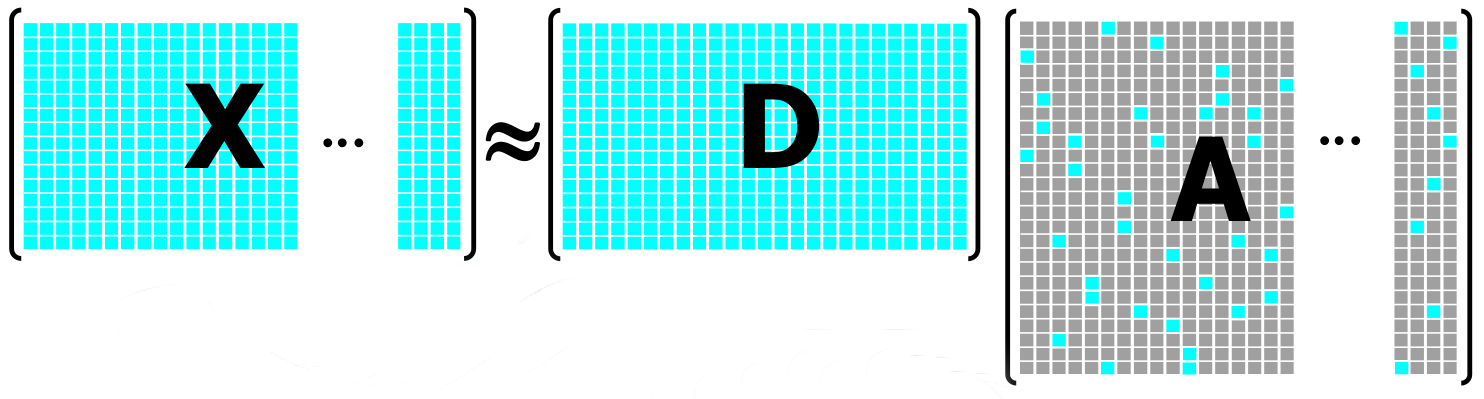
\includegraphics[width=0.9\textwidth]{./figures/DL/dict_rep.png}
		\vspace*{-0.5cm}	
		\end{figure}
		{\hfill \tiny (photo credit: Rubinstein)}
				
		\item Dictionary learning as an alternating optimization problem:
		\begin{equation*}
			\left(\dict, \dictco\right)  = \argmin_{\dict,\dictco} \left\lbrace \Vert \X-\dict \dictco\Vert^2_2 + \lambda \Vert \dictco \Vert_1 \right\rbrace
		\end{equation*}
	\end{itemize}
\end{frame}

\begin{frame}
	\frametitle{Orthogonal vs redundant bases} 
	\begin{minipage}{\textwidth}
		\begin{minipage}[b]{0.41\textwidth}
			\begin{figure}
				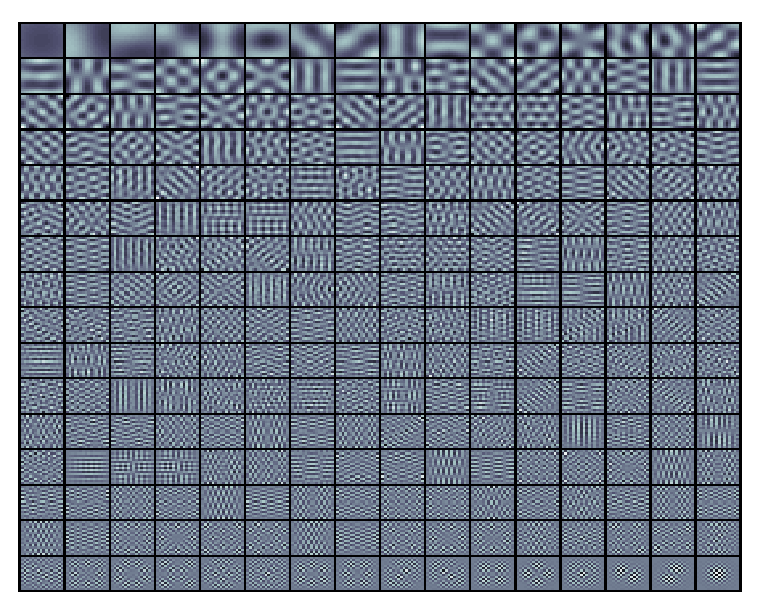
\includegraphics[width=\columnwidth]{./figures/DL/dictionary_PCA_patchsize04.eps}
			\end{figure}
		\end{minipage}
		\hfil
		\begin{minipage}[b]{0.57\textwidth}
			\begin{figure}
				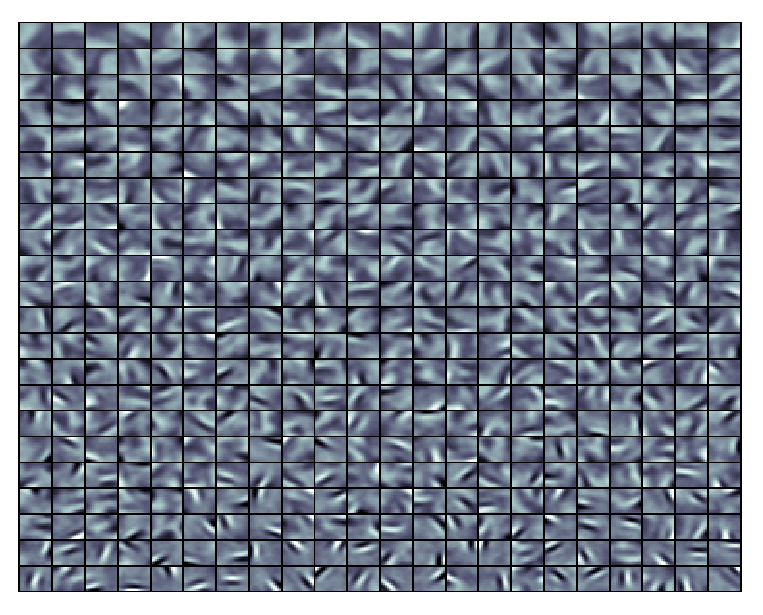
\includegraphics[width=\columnwidth]{./figures/DL/dictionary_ODL_patchsize04_full.eps}
			\end{figure}
		\end{minipage}	
	\vspace{0.5cm}	
	\centering \scriptsize Dictionaries learned by POD and DL from the set of HR patches of size $ 16 \times 16 $
	\end{minipage}
\end{frame}

\begin{frame}
	\frametitle{Reconstruct HR fields using coupled dictionary learning} 
	\begin{itemize} \itemsep0em
		\item Motivated by single image super-resolution {\footnotesize \cite{yang2010image}}
		\item Two steps: \emph{learning} (offline) and \emph{reconstruction} (online)
	\end{itemize}
	\vspace{-0.25cm}
	\begin{figure} 
		\begin{overprint}
		\onslide<1>	\centering
		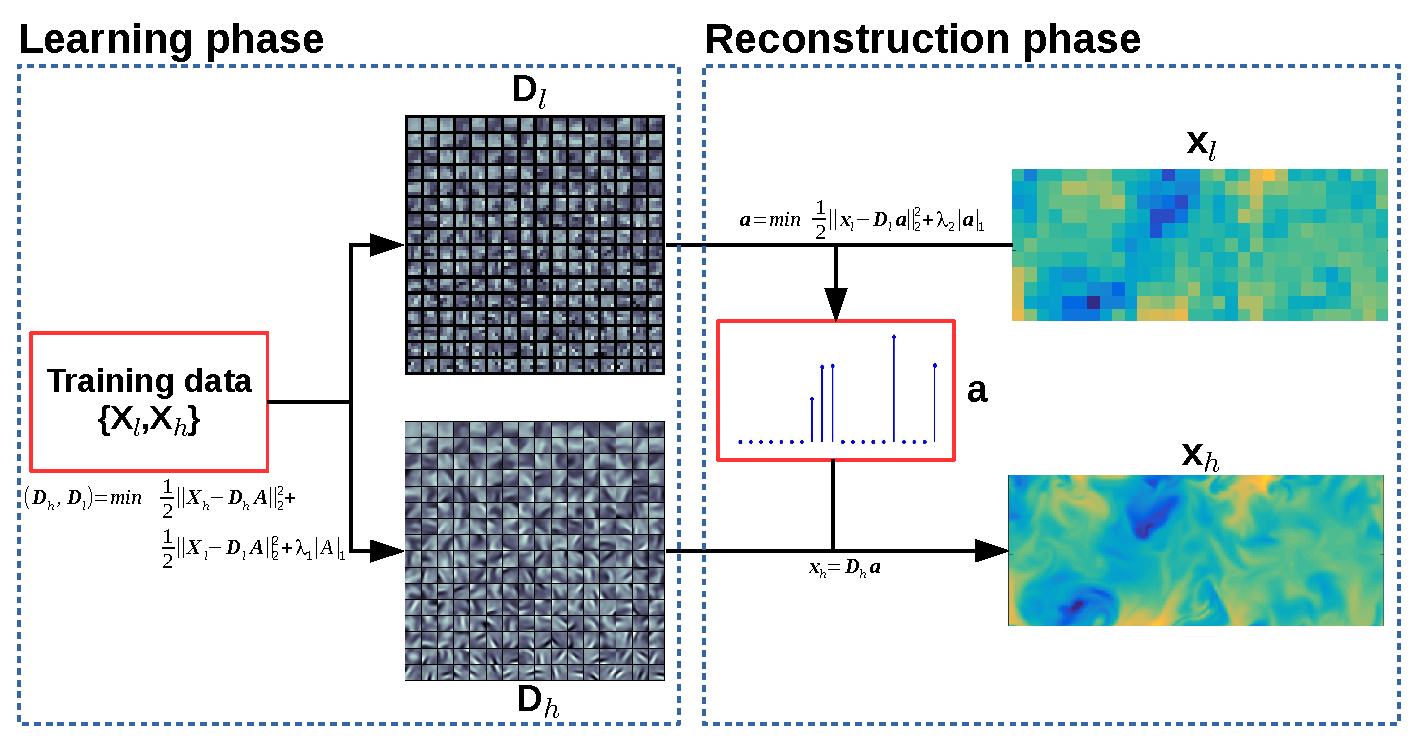
\includegraphics[width=\textwidth]{./figures/DL/SR_skeme.pdf}
		\onslide<2>	\centering
		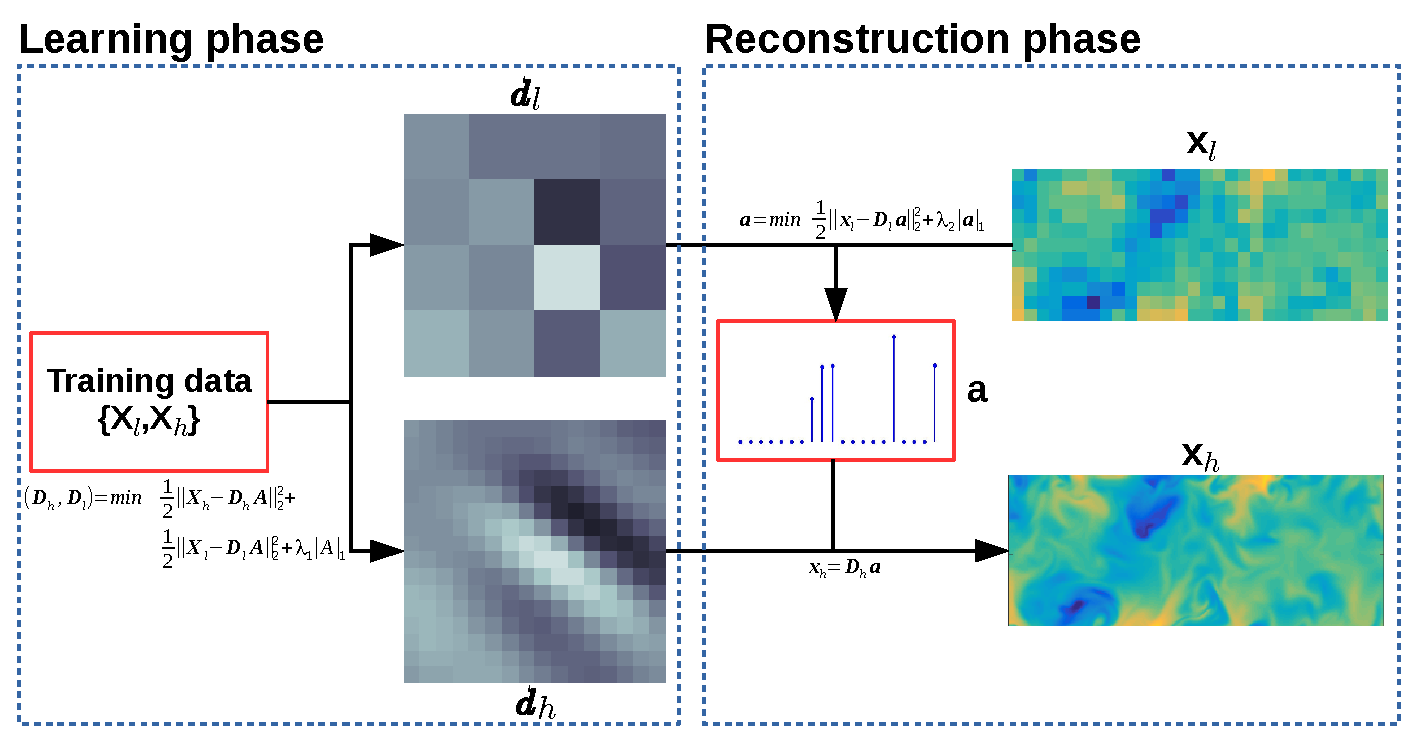
\includegraphics[width=\textwidth]{./figures/DL/SR_skeme_zoom.pdf}		
		\onslide<3>	\centering
		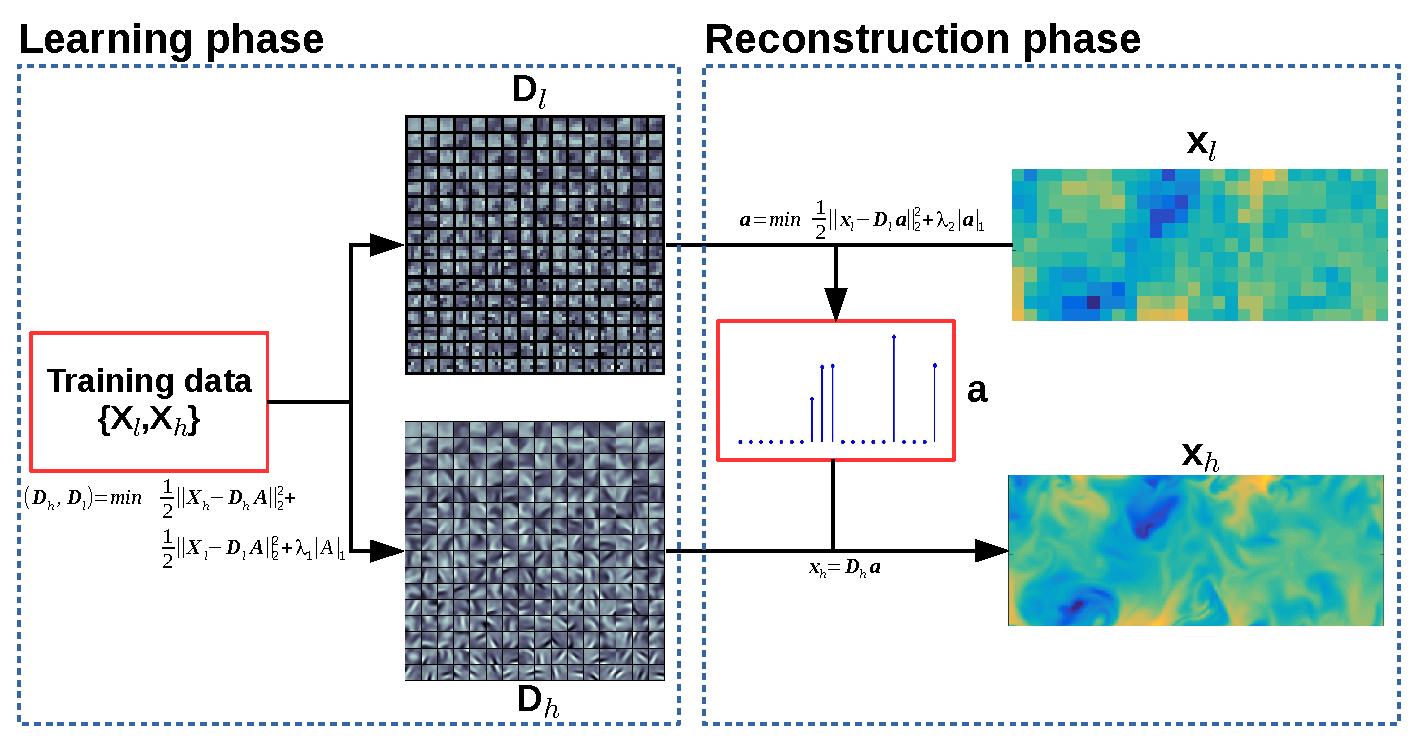
\includegraphics[width=\textwidth]{./figures/DL/SR_skeme.pdf}
		\end{overprint}
	\end{figure}
\end{frame}

\begin{frame}
	\frametitle{Numerical experiment setup for coupled dictionary learning} 
	\begin{itemize} %\itemsep0em
	\item \textbf{Subsampling}: $ \y_t \mydef \Sub_s\z_t $
	
	\item \textbf{Downsampling case}: $ \y_t \mydef \Sub_s\LPF_s\z_t $
	\item \textbf{Patch-based approach}: localized information
	\item \textbf{Parameters}: patch size, number of patches, sparsity constraints (for the learning and reconstruction step)
	\item \textbf{Preprocessing methods} by coupling:
		\begin{itemize}
			\item High and low resolution, $ \left\lbrace \textcolor{red}{\z_t}, \textcolor{blue}{\y_t} \right\rbrace $
			\item Reference and interpolated high resolution, $ \left\lbrace \textcolor{red}{\z_t}, \textcolor{blue}{\Interp_s\y_t} \right\rbrace $
			\item Residual and features (derivatives), $ \left\lbrace \textcolor{red}{\z_t - \Interp_s\y_t}, \textcolor{blue}{\varmathbb{F} \Conv \Interp_s\y_t} \right\rbrace $
		\end{itemize}
	\end{itemize}
\end{frame}

\begin{frame}
	\frametitle{Results: energy spectra} 

	\begin{figure}
		\centering 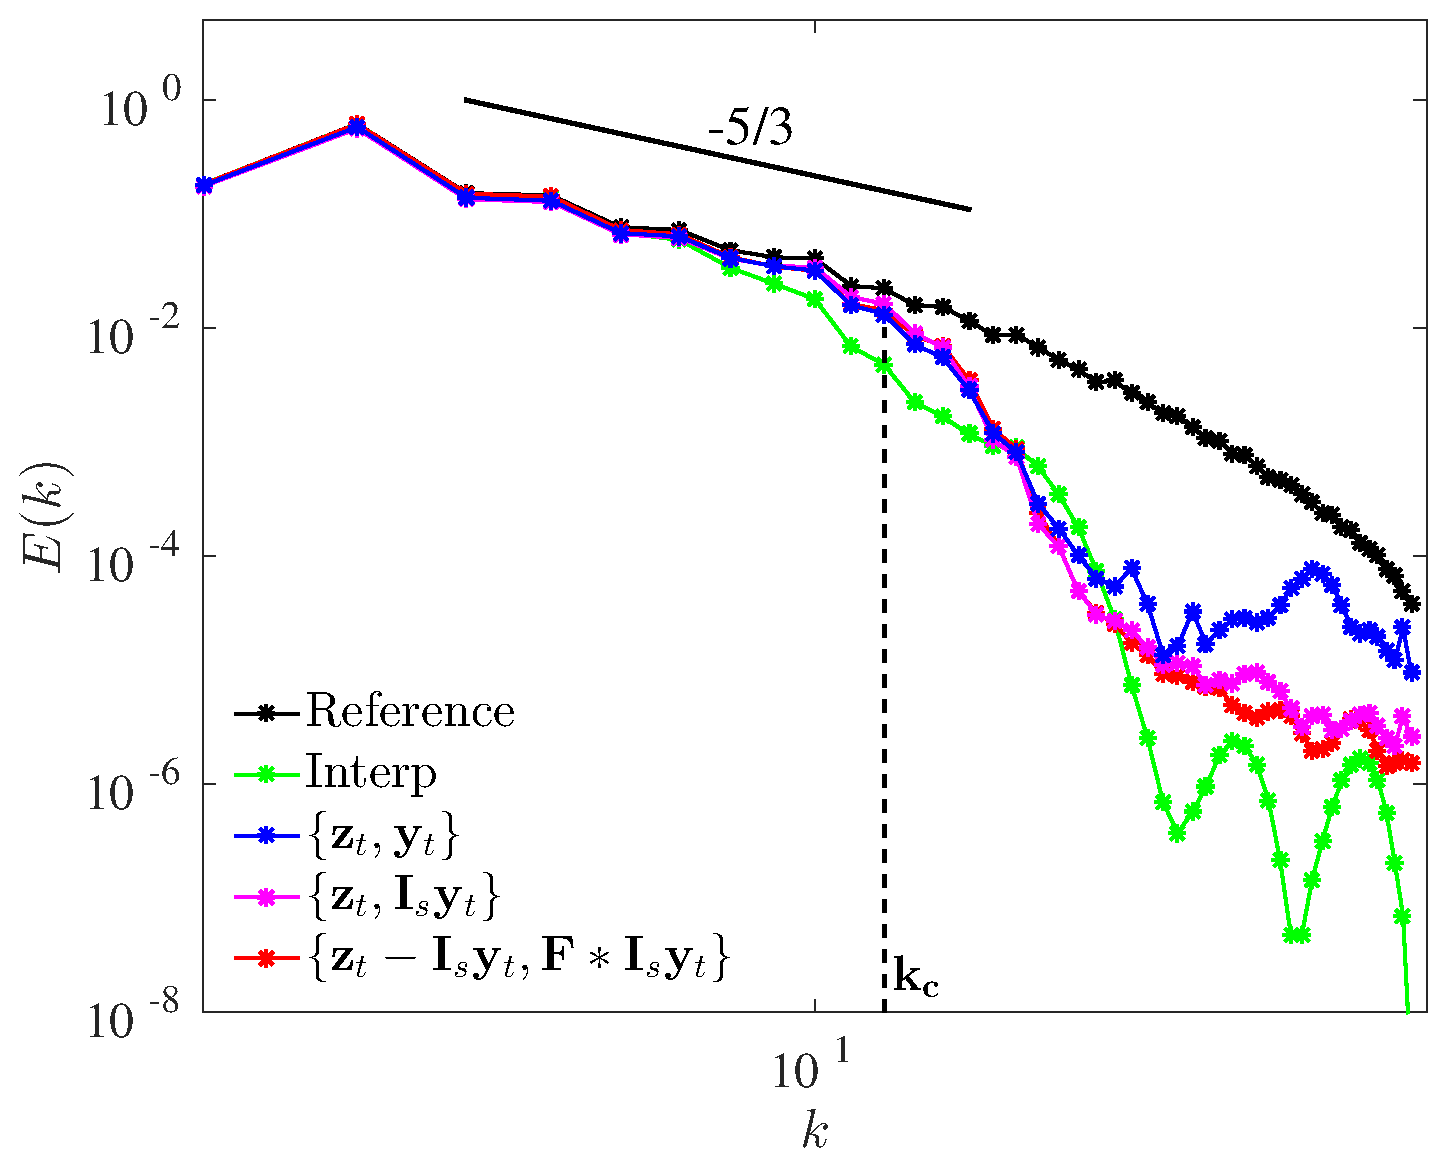
\includegraphics[width=0.65\textwidth]{./figures/DL/spectra2d_spacespacing_04.eps}
		\caption*{Energy spectra (2D) of reference, interpolation and reconstruction by 3 coupled dictionary learning approaches (sampling ratio of $ 4 \times 4 $)}
	\end{figure}
\end{frame}

\begin{frame}
	\frametitle{Results: spectra of the error} 

	\begin{figure}
		\centering
		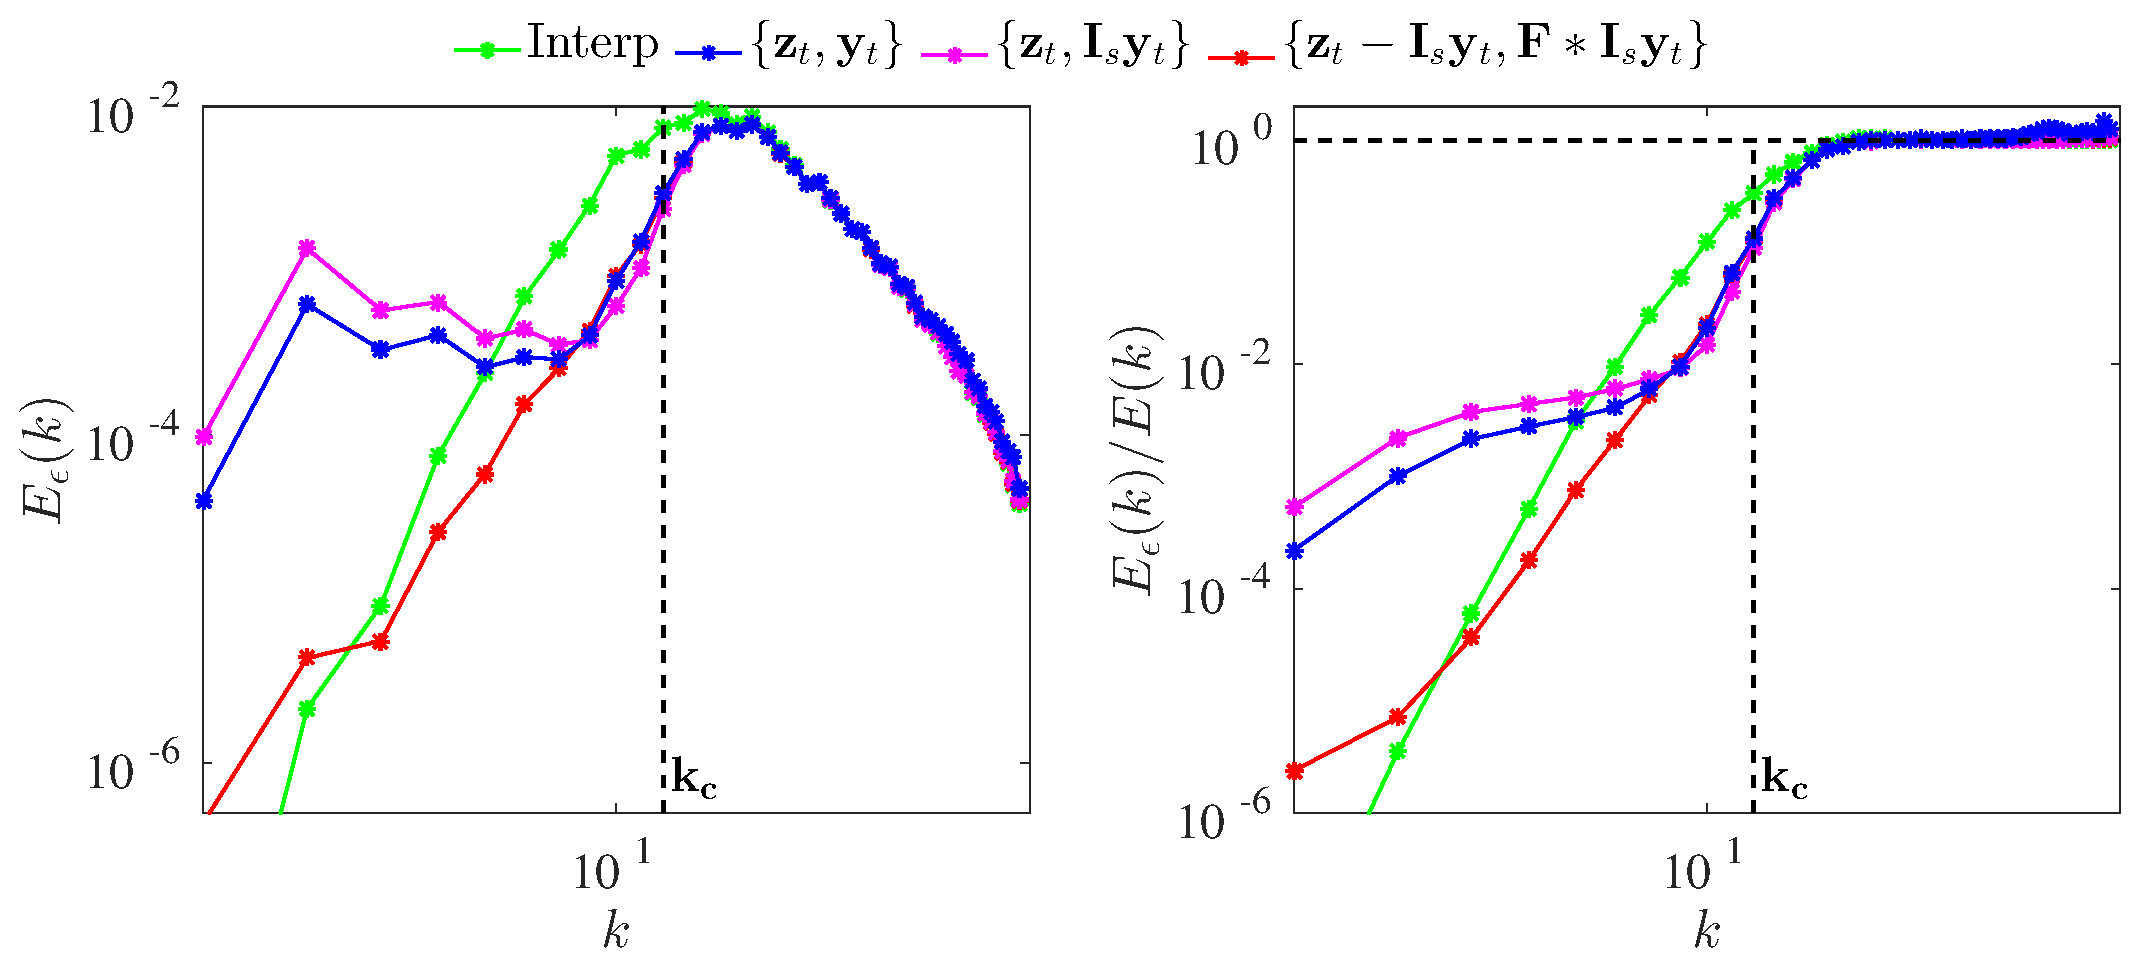
\includegraphics[width=\textwidth]{./figures/DL/errspectra2d_nonnormalized_normalized_timespacing_06_spacespacing_04.eps}
		\caption*{2D error spectra (with and without normalization) of interpolation and reconstruction by 3 coupled dictionary learning approaches (sampling ratio of $ 4 \times 4 $)}
	\end{figure}
\end{frame}

% % % % % % % % % % % % % % % % % % % % % % % % % % % % % % % % % % % % % % % % % % % % % %
\subsection{Fusion of complementary measurements}		
\begin{frame}
\frametitle{A generalization of non-local means}	
	\begin{tcolorbox}[colback=red!5!white,colframe=red!75!black]	
		\textbf{Objective}: propagating small scales from LTHS planes based on the similarity levels between large scales 
 	\end{tcolorbox}
 	\vfill
	\centering
	\only<1>{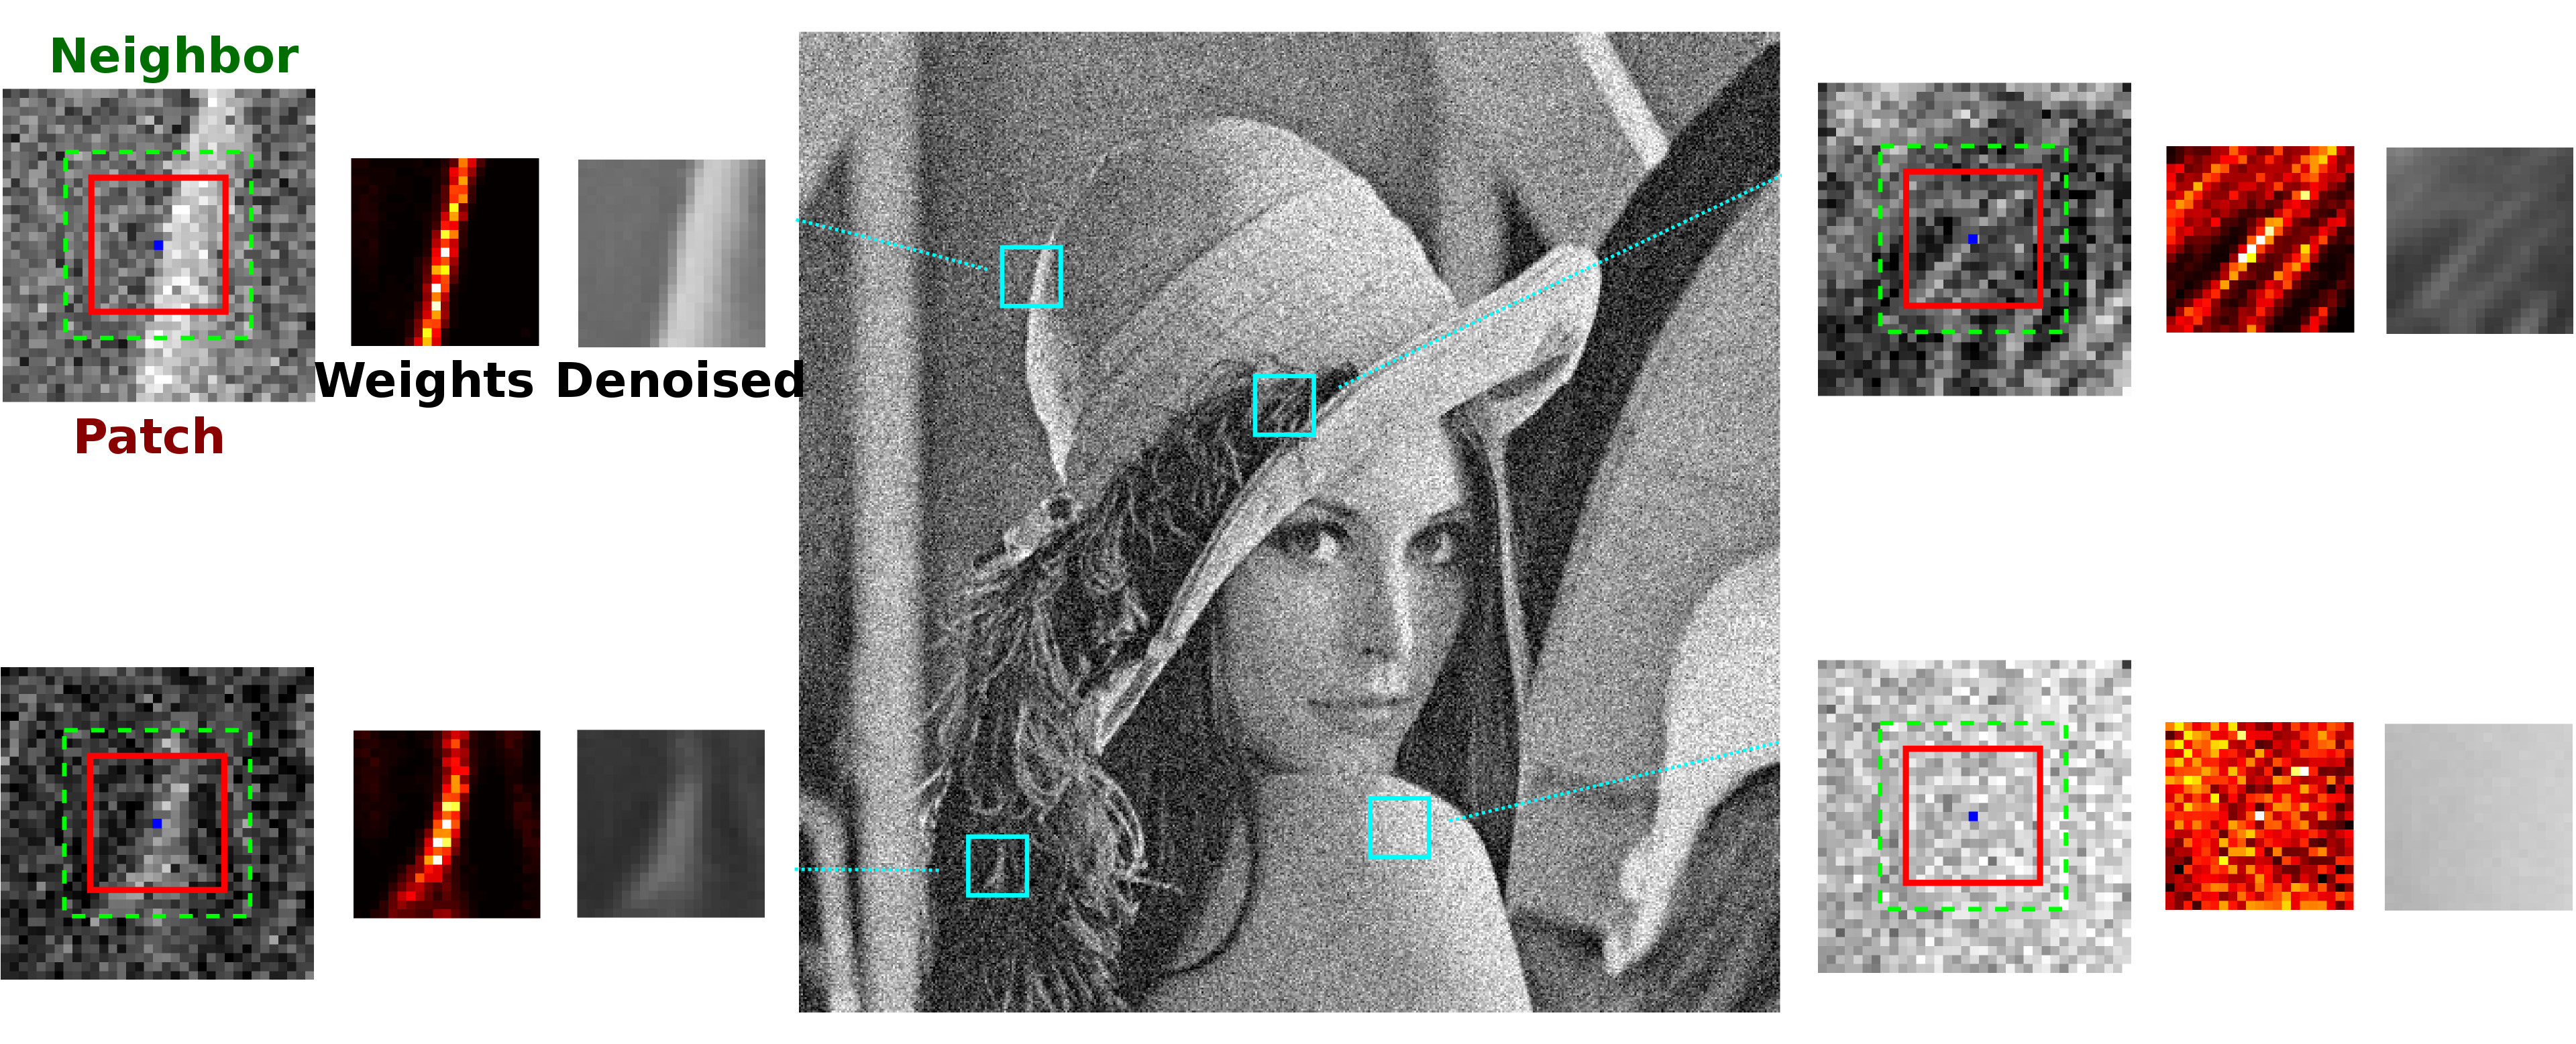
\includegraphics[height=4.75cm]{./figures/NLM/lena.png}\captionof{figure}{Non-local means for denoising \cite{buades2005review}}}
	\only<2>{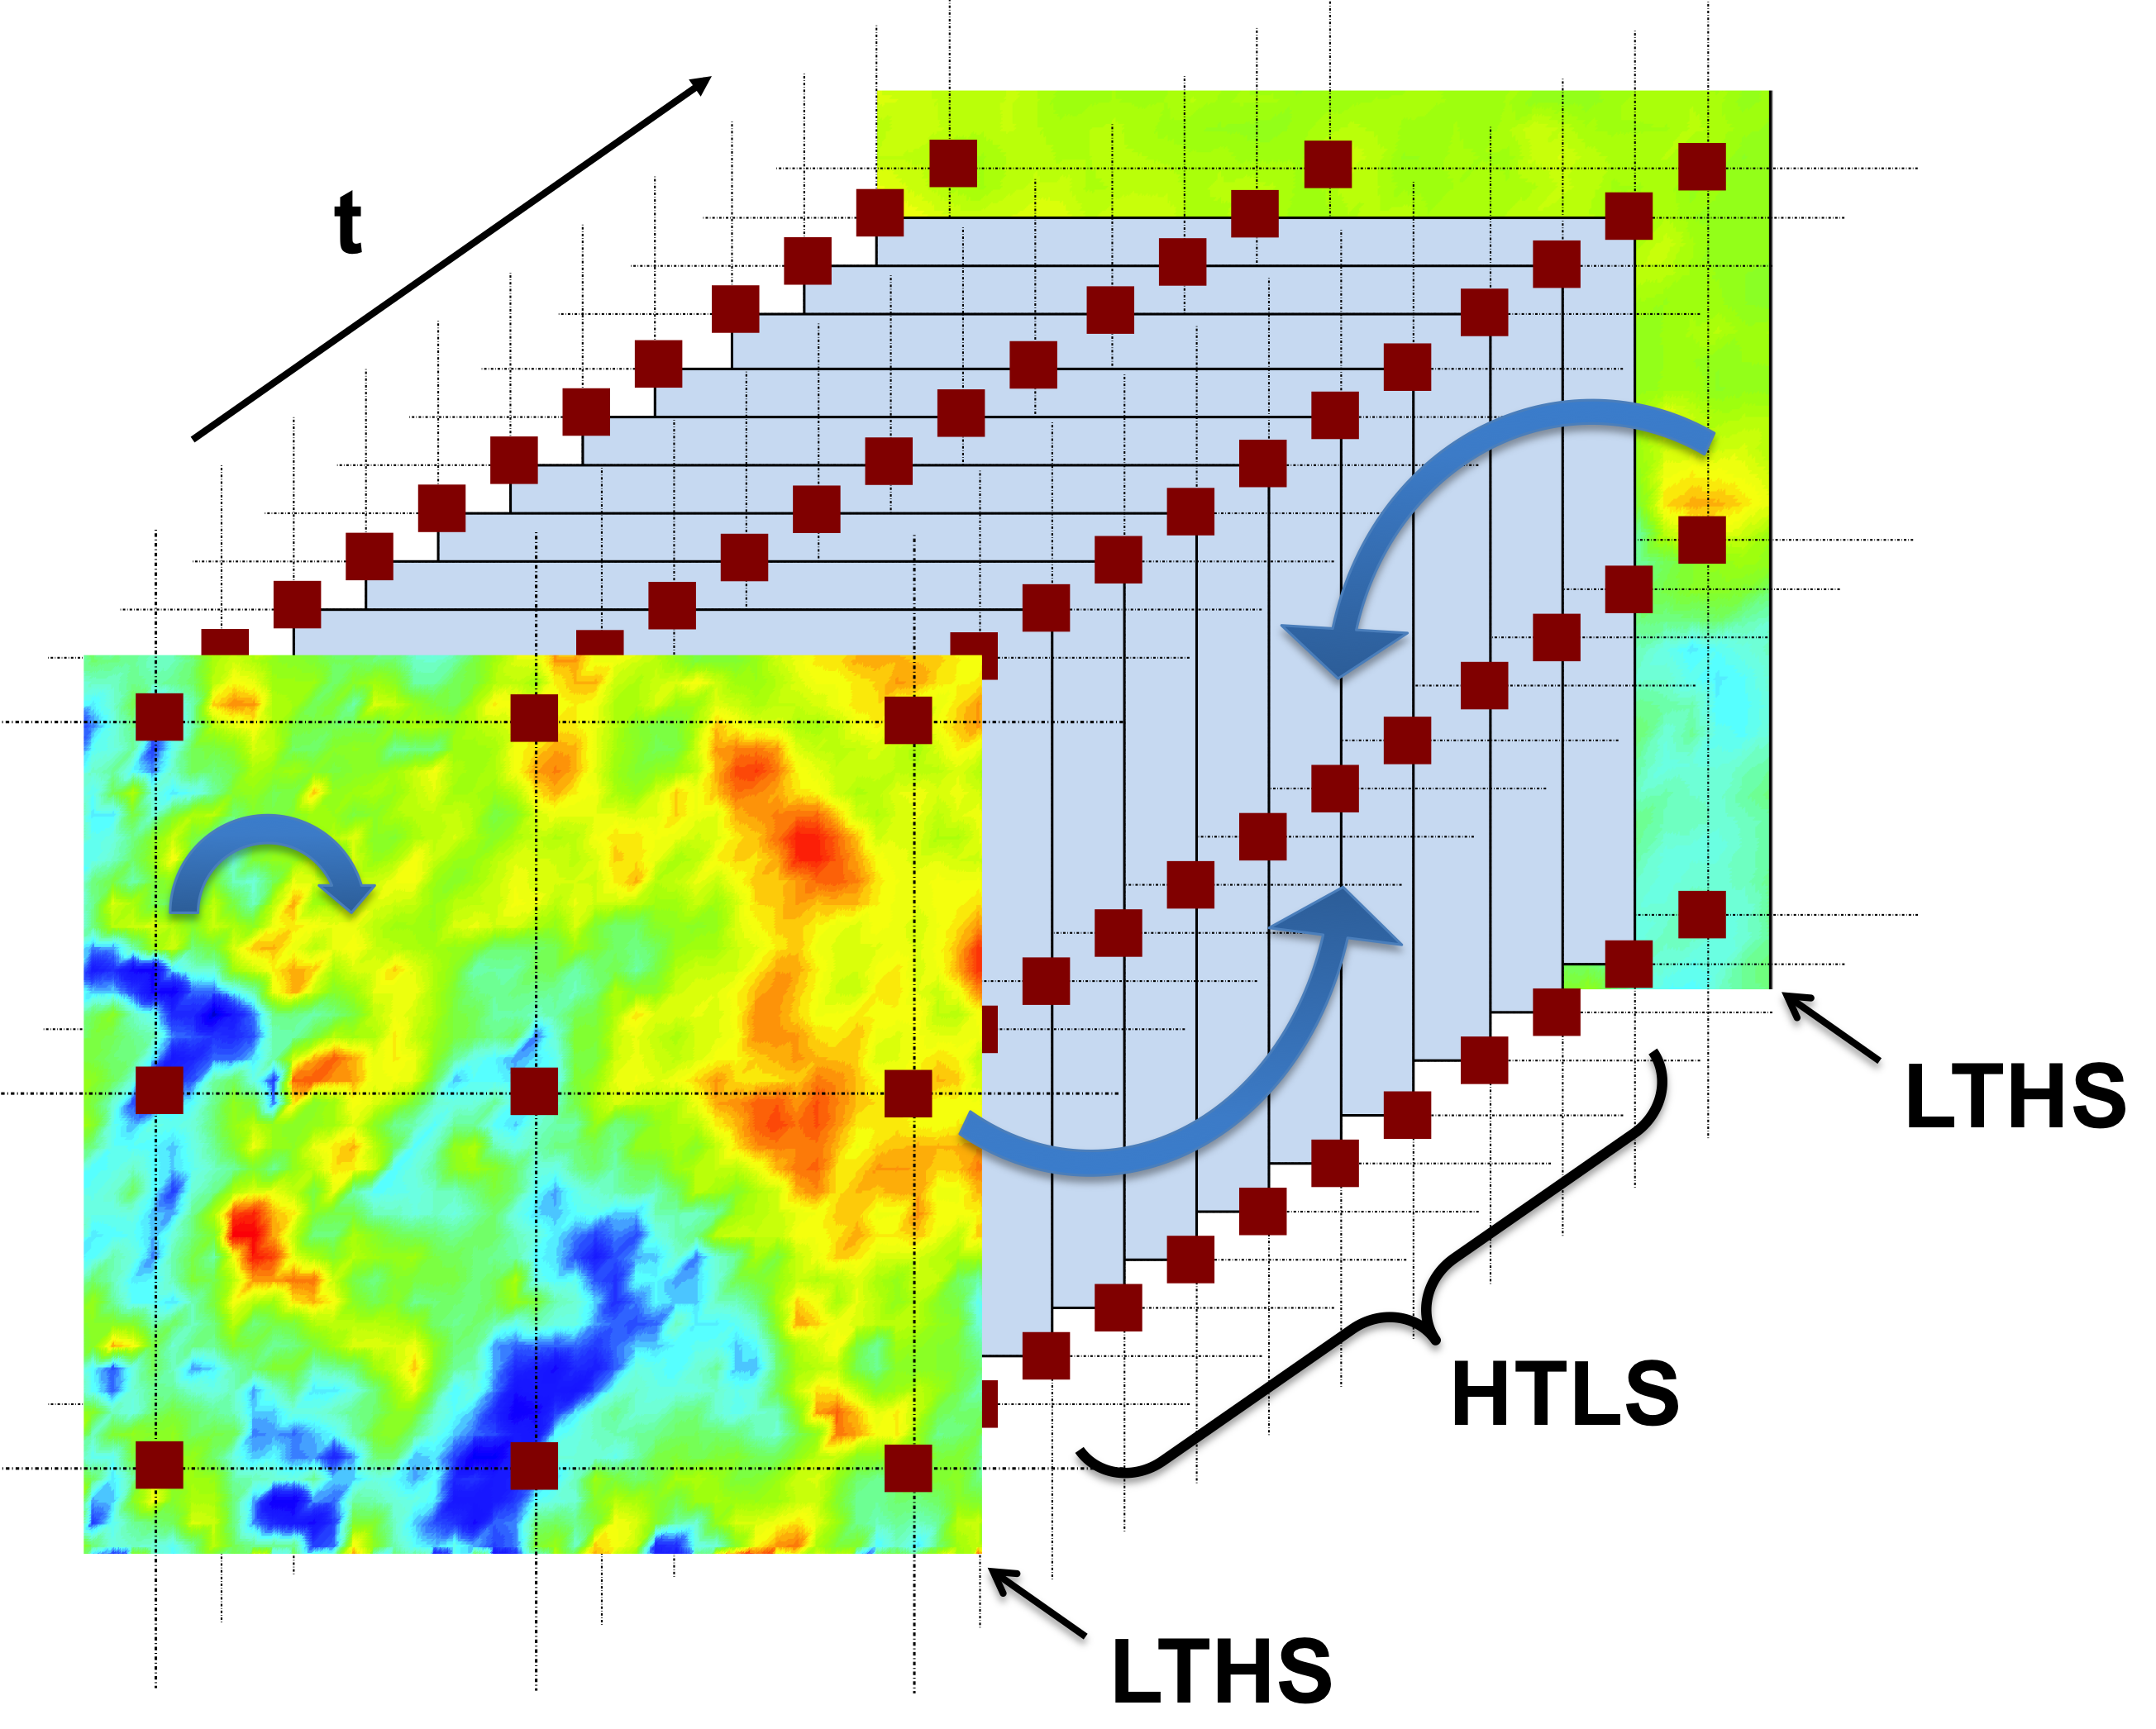
\includegraphics[height=4.75cm]{./figures/experimentalsetup/experiment_setup_fusion.png}\captionof{figure}{Propagation of small scales, inspired by video super-resolution \cite{protter2009generalizing}}}
\end{frame}

\begin{frame}
\frametitle{The principle: weighted average using non-local similarity}
	\begin{itemize}\itemsep0em
		\item \textbf{Principle}: video super-resolution {\footnotesize \cite{protter2009generalizing}}
		\begin{equation*}
			\tcbhighmath[boxrule=2pt,drop fuzzy shadow=blue]{\textcolor{blue}{\hat{\mybold{z}}_{t_\knot}}[k]=\frac{\sum_{t\in\neighbor_{t_\knot}}\sum_{i\in\neighbor_k}w[k,i,t]\textcolor{blue}{\mybold{y}_t}[i]}{\displaystyle \sum_{t\in\neighbor_{t_\knot}}\sum_{i\in\neighbor_k}w[k,i,t]}}
		\end{equation*}
		where $ w[k,i,t] = \myexp{ -\frac{1}{2\nlmfilparam^2} \Vert \mathcal{R}_s^k\mybold{y}_{t_\knot}-\mathcal{R}_s^i\mybold{y}_t \Vert^2_2} $
		\vspace{0.2cm}
		\item \textbf{Modification}: reconstruct small scales $ \boundHF_{t_\knot} = \mybold{x}_{t_\knot} - \Interp_s\Sub_s\mybold{x}_{t_\knot} $ only
		\begin{minipage}{\textwidth}
			\begin{minipage}{0.7\textwidth}
				\begin{equation*}
					\textcolor{blue}{\hat{\h}_t}[k]=\frac{\sum_{i\in\neighbor_k}w_0[k,i,t]\textcolor{blue}{\boundHF_{t_\knot}}[i] + \sum_{i\in\neighbor_k}w_1[k,i,t]\textcolor{blue}{\boundHF_{t_\knot+1}}[i]}{\displaystyle\sum_{i\in\neighbor_k}w_0[k,i,t] + \sum_{i\in\neighbor_k}w_1[k,i,t]}
				\end{equation*}
			\end{minipage}
			\hfill
			\begin{minipage}{0.25\textwidth}
				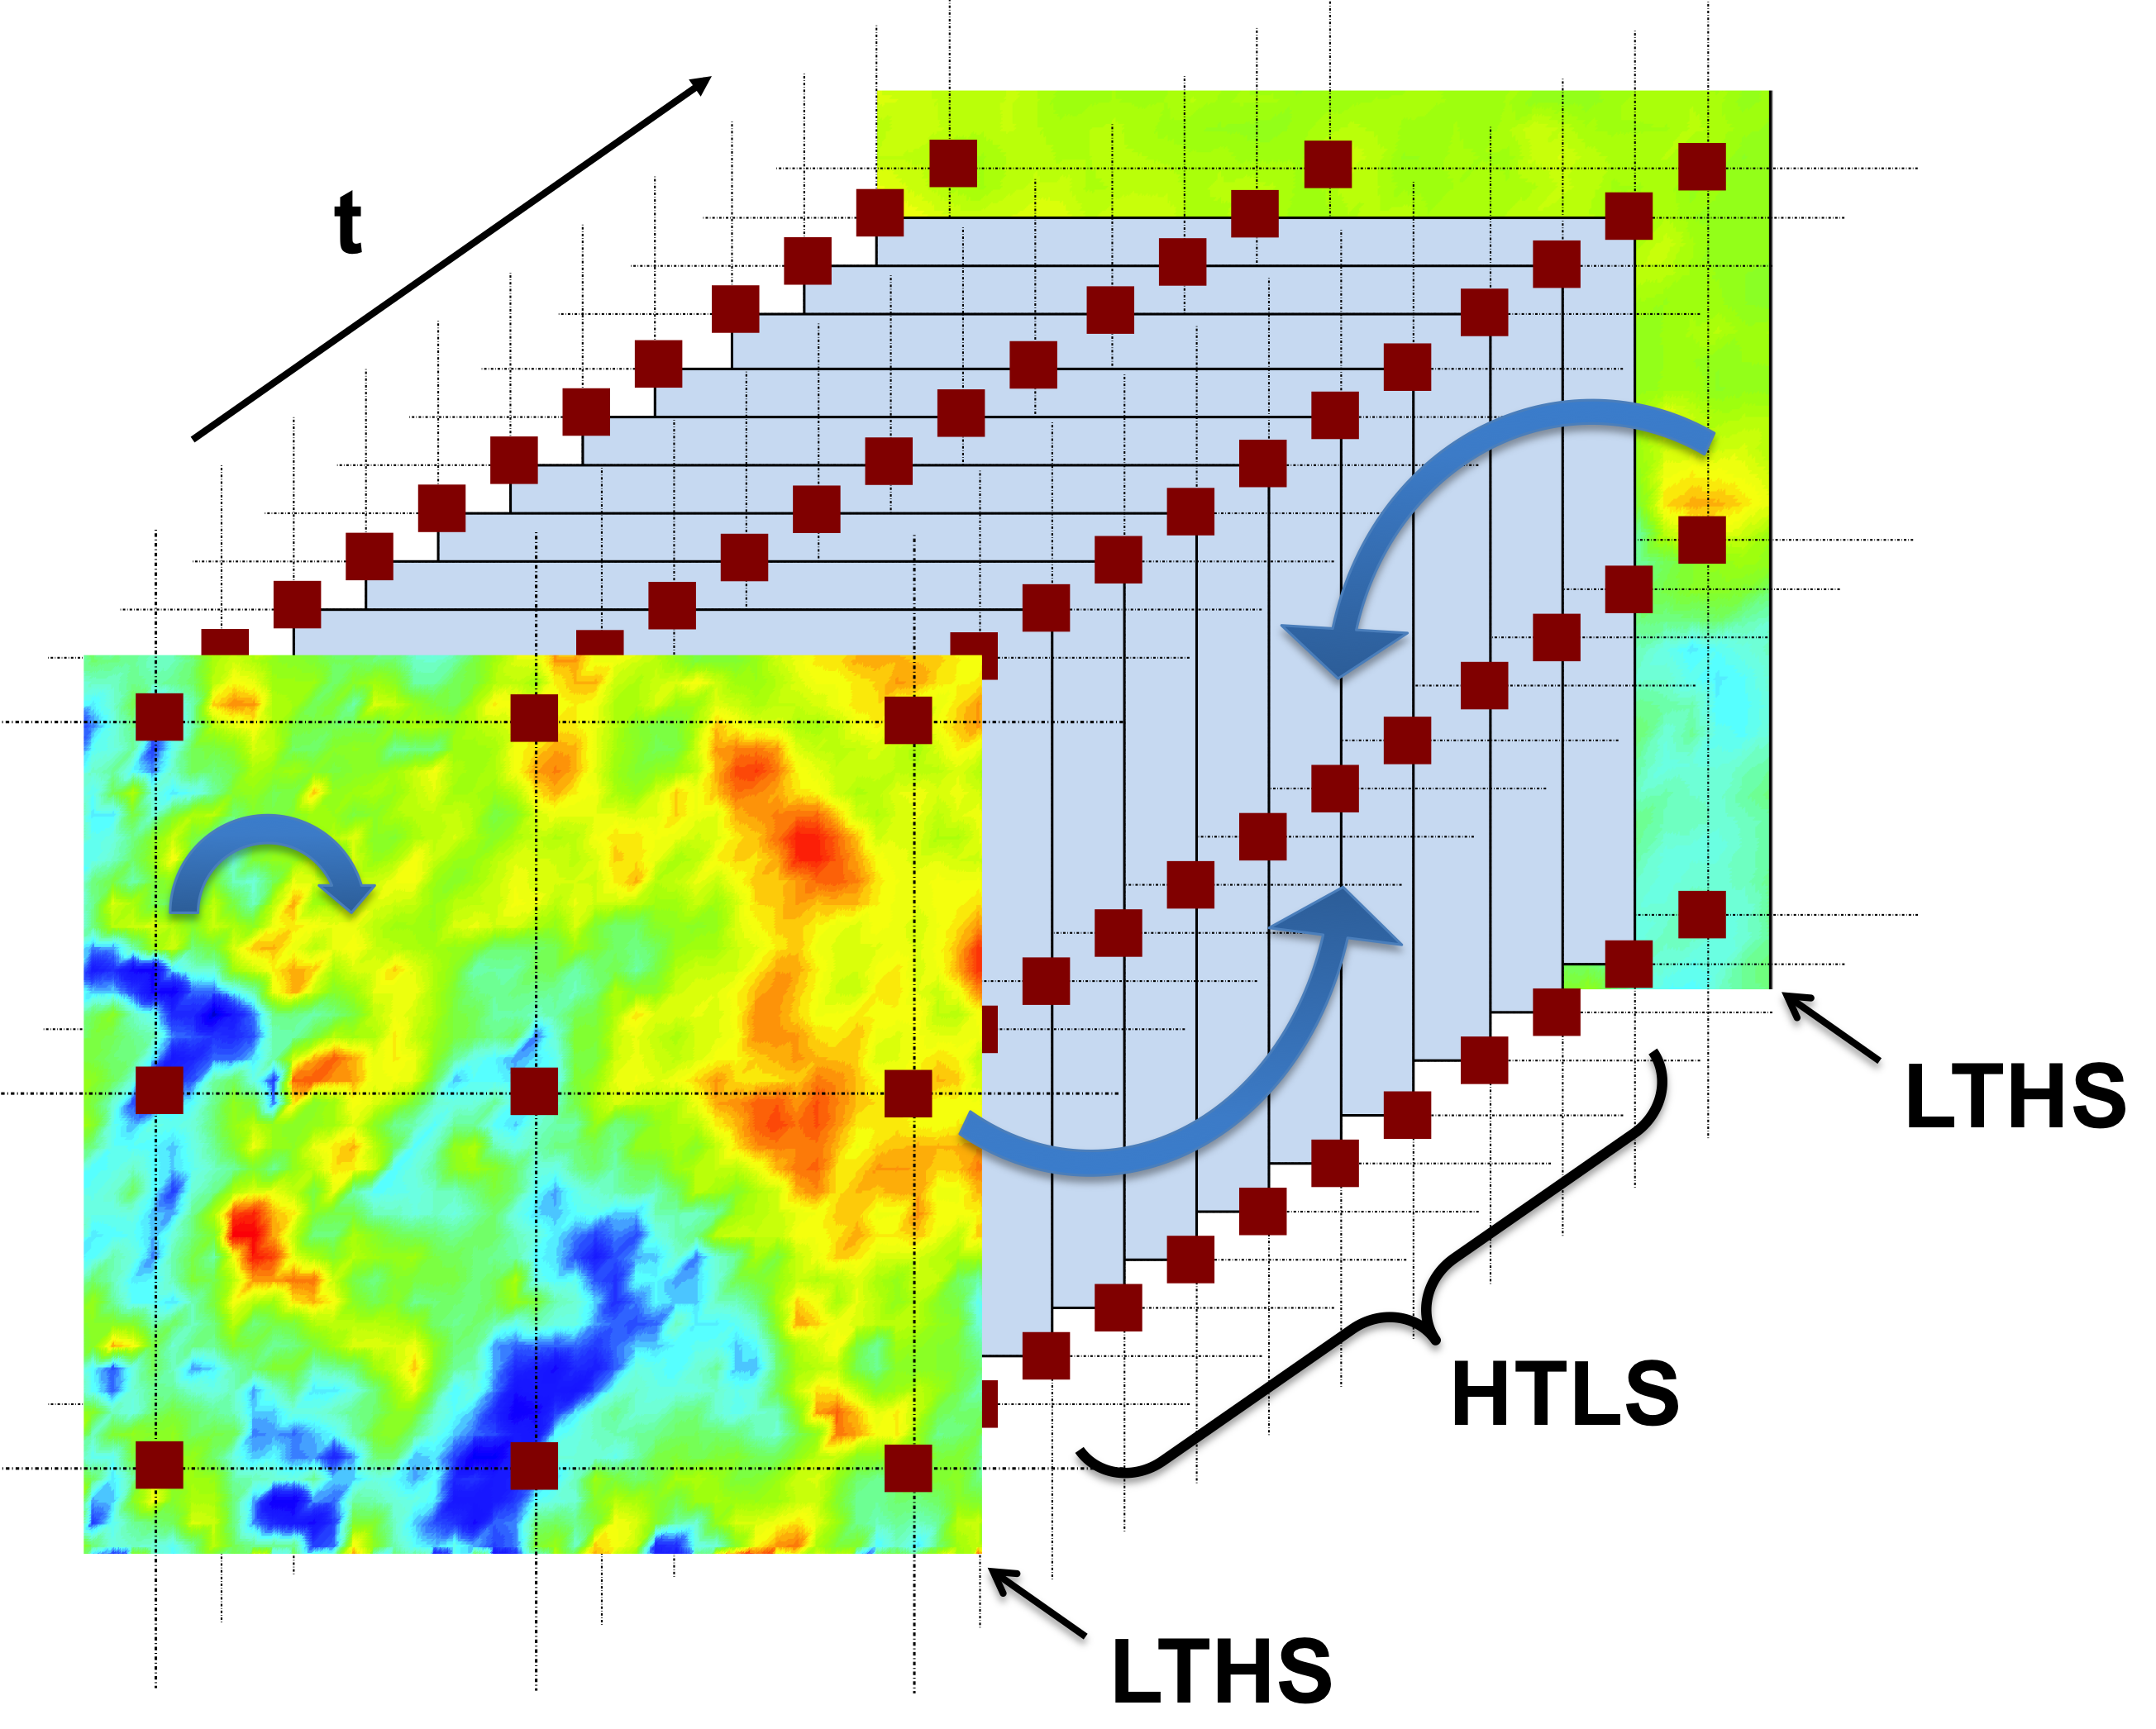
\includegraphics[height=1.75cm]{./figures/experimentalsetup/experiment_setup_fusion.png}
			\end{minipage}			
		\end{minipage}		
	\end{itemize}
\end{frame}

\begin{frame}
\frametitle{Non-local means: schemes and parameters}
	\begin{itemize}
		\item \textbf{Parameters}: 
			\begin{itemize}
				\item Filter parameter: $ \sigma $
				\item Neighbor sizes $ \# \left( \neighbor_k \right)$
				\item Patch size: $ \# \left(\mathcal{R}_s^k\mybold{y}_t\right) $
			\end{itemize}	
		\item \emph{Greedy} and \emph{non-greedy} propagation schemes
		\begin{figure}
		\centering
			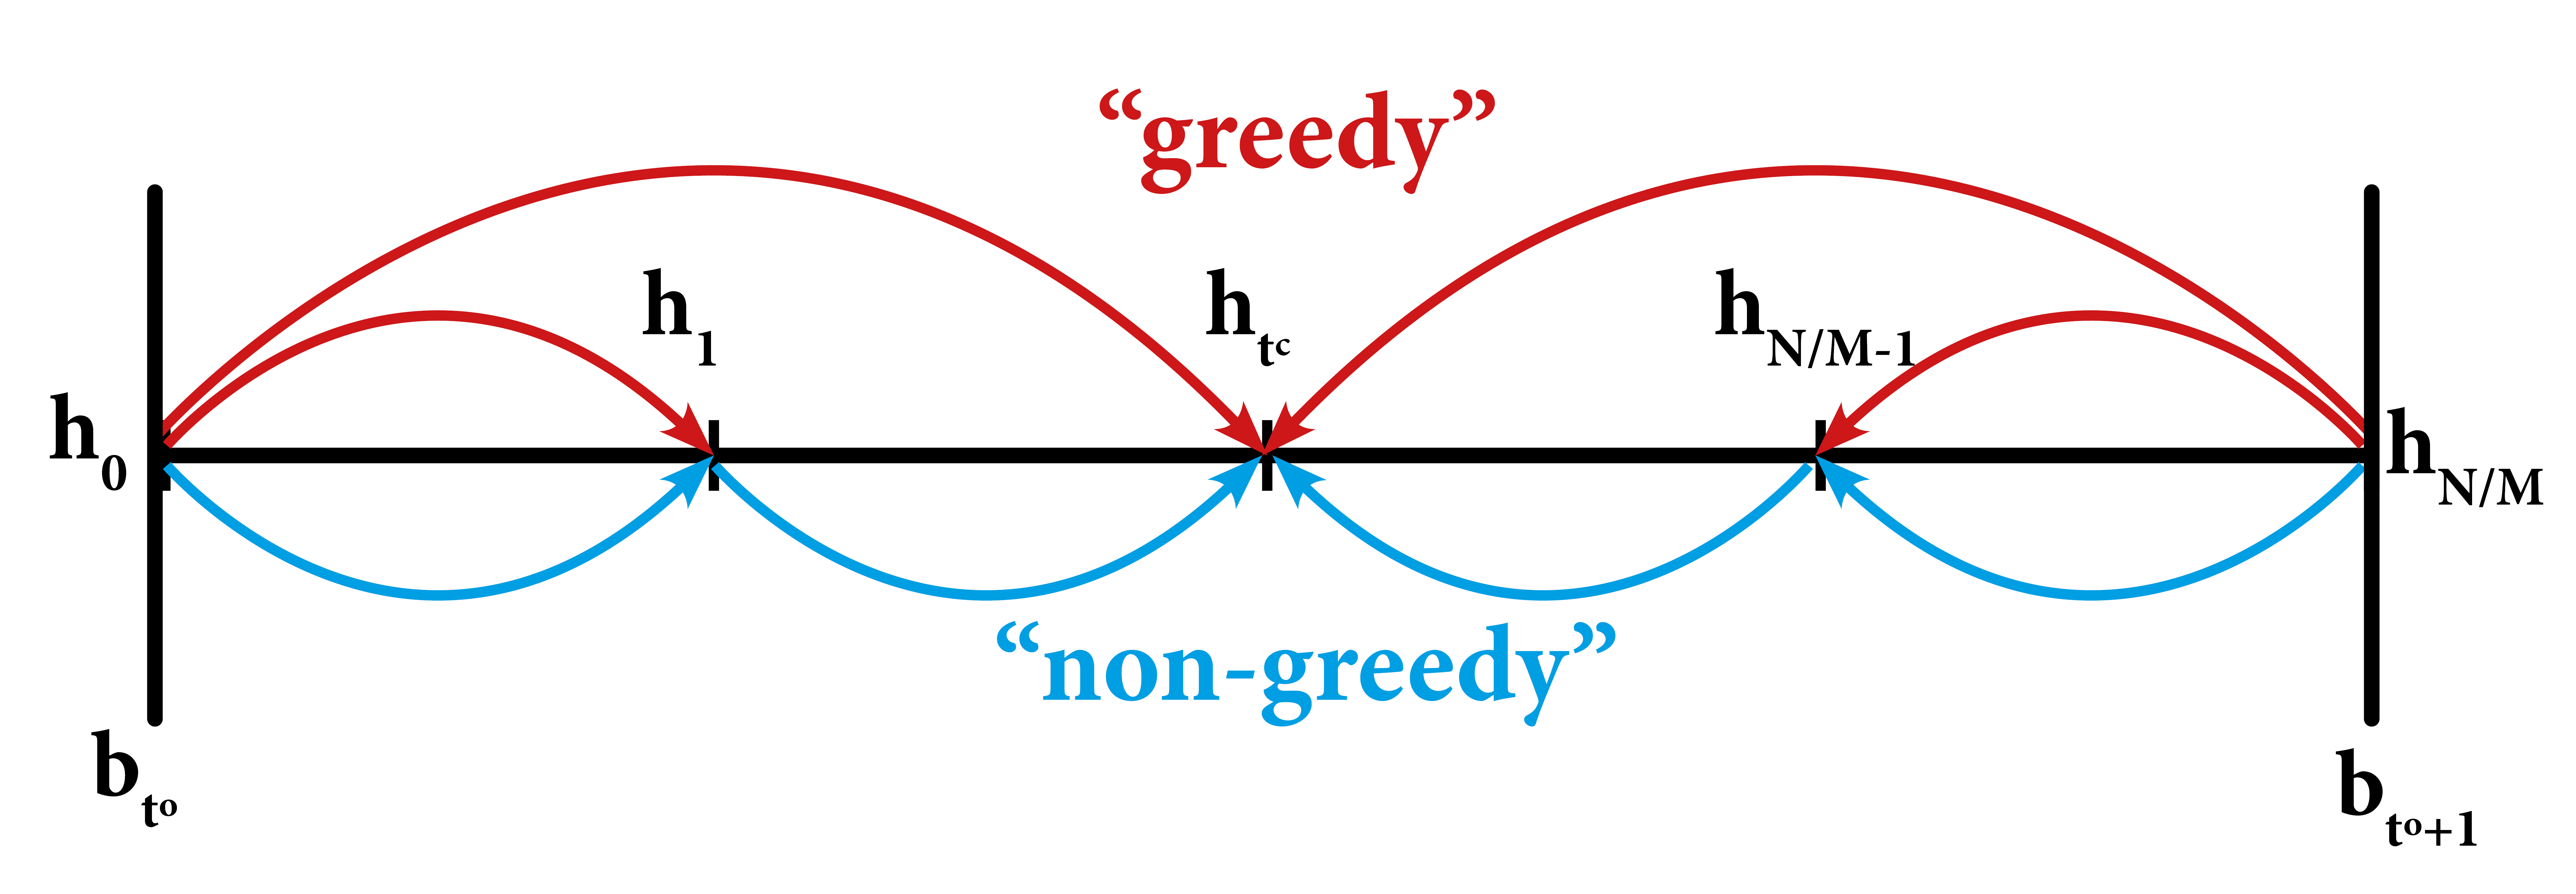
\includegraphics[width=0.8\columnwidth]{./figures/NLM/propagation_scheme.png}
			\vspace{-0.3cm}
		\end{figure}	
	\end{itemize}
\end{frame}

\begin{frame}
\frametitle{Bayesian fusion: the framework}
	\begin{itemize}\itemsep0em
		\item Motivation: fusion of multi- and hyper-spectral images {\footnotesize \cite{hardie2004map}}
		\item Bayesian fusion:  \textit{maximum a posteriori}
		\begin{equation*}
		 \hat{\z}=\argmax_{\z} \left\lbrace  p \left(\z|\x,\y\right) \right\rbrace 
		\end{equation*} 

		\item Applying \emph{Bayes' theorem}:
		\begin{equation*}
			p\left(\z|\x,\y\right) = \frac{p\left( \x,\y|\z\right)p\left( \z\right)}{p\left( \x,\y\right)} = \frac{p\left( \x|\z\right) p\left( \y|\z\right) p\left( \z\right) }{p\left( \x,\y\right)}
		\end{equation*} 	
		 
		\item \emph{Non-informative} (\emph{improper}) prior, i.e. $ p\left( \z\right) $ is constant,: 
		\begin{equation*}
				\tcbhighmath[boxrule=2pt,drop fuzzy shadow=blue]{\hat{\z} = \argmax_{\z}\left\lbrace p\left( \z|\x\right) p\left( \z|\y\right)\right\rbrace}
		\end{equation*} 	
	\end{itemize}
\end{frame}

\begin{frame}
\frametitle{Single models and closed-form fusion formula} 
	\begin{itemize}\itemsep0em
		\item Single models:
		\begin{equation*}
			\begin{split}
			\z &= \varmathbb{I}_t\x+\boldsymbol{h}_t  \:\:\:\:\: (\varmathbb{I}_t\x \indep \boldsymbol{h}_t)\\
			\z &= \varmathbb{I}_s\y+\boldsymbol{h}_s \:\:\:\: (\varmathbb{I}_s\y \indep \boldsymbol{h}_s)	
			\end{split}	
		\end{equation*}
		
		\item Multivariate Gaussian probability: 
		\begin{equation*}
			p(\z|\x) = \frac{1}{(2\pi)^{\dimsh\dimth/2}\left| \Sigma_{\boldsymbol{h}_t} \right|^{1/2} } \exp \left\lbrace -\frac{1}{2} \left( \z-\varmathbb{I}_t\x \right)^{\mytrans} \Sigma_{\boldsymbol{h}_t}^{-1} \left( \z-\varmathbb{I}_t\x \right)\right\rbrace
		\end{equation*}	
		{\centering ($ \Sigma_{\boldsymbol{h}_t}= \boldsymbol{h}_t \boldsymbol{h}_t^{\mytrans}$: covariance matrix)}
		
		\item Closed-form solution:
		\begin{equation*}
		\tcbhighmath[boxrule=2pt,drop fuzzy shadow=blue]{\textcolor{blue}{\hat{\z}}=\left(\Sigma_{\boldsymbol{h}_s}^{-1}+\Sigma_{\boldsymbol{h}_t}^{-1}\right)^{-1} \left(\Sigma_{\boldsymbol{h}_s}^{-1}\textcolor{blue}{\varmathbb{I}_s\y}+\Sigma_{\boldsymbol{h}_t}^{-1}\textcolor{blue}{\varmathbb{I}_t\x}\right)}
		\end{equation*} 	
	\end{itemize}
\end{frame}

\begin{frame}
\frametitle{Simplification and interpretation of the fusion formula} 
	\textbf{Simplification}: $ \Sigma_{\boldsymbol{h}_s} $ and $ \Sigma_{\boldsymbol{h}_t} $ are diagonal
	\begin{equation*}
		\tcbhighmath[boxrule=2pt,drop fuzzy shadow=blue]{\textcolor{blue}{\hat{\z }}[i,t]=\frac{\mybold{\sigma}^2_{\h_s}[i,t]}{\mybold{\sigma}^2_{\h_s}[i,t]+\mybold{\sigma}^2_{\h_t}[i,t]}\textcolor{blue}{\Interp_t\x} [i,t]+\frac{\mybold{\sigma}^2_{\h_t}[i,t]}{\mybold{\sigma}^2_{\h_s}[i,t]+\mybold{\sigma}^2_{\h_t}[i,t]}\textcolor{blue}{\Interp_s\y} [i,t]}
	\end{equation*} 
	\pause
	\begin{minipage}{\columnwidth}
		\begin{minipage}{0.55\columnwidth} 
			\textbf{Interpretation}: $ \hat{\z}$ is fused from 2 data sources $\Interp_t\x$ and $\Interp_s \y$ via weighted coefficients $ \boldsymbol{\sigma}^2_{\boldsymbol{h}_s} $ and $ \boldsymbol{\sigma}^2_{\boldsymbol{h}_t} $ (learned from $ \x $ and $ \y $ only).
		\end{minipage}	
		\hspace{0.5cm}
		\begin{minipage}{0.3\columnwidth}
			\begin{figure}
				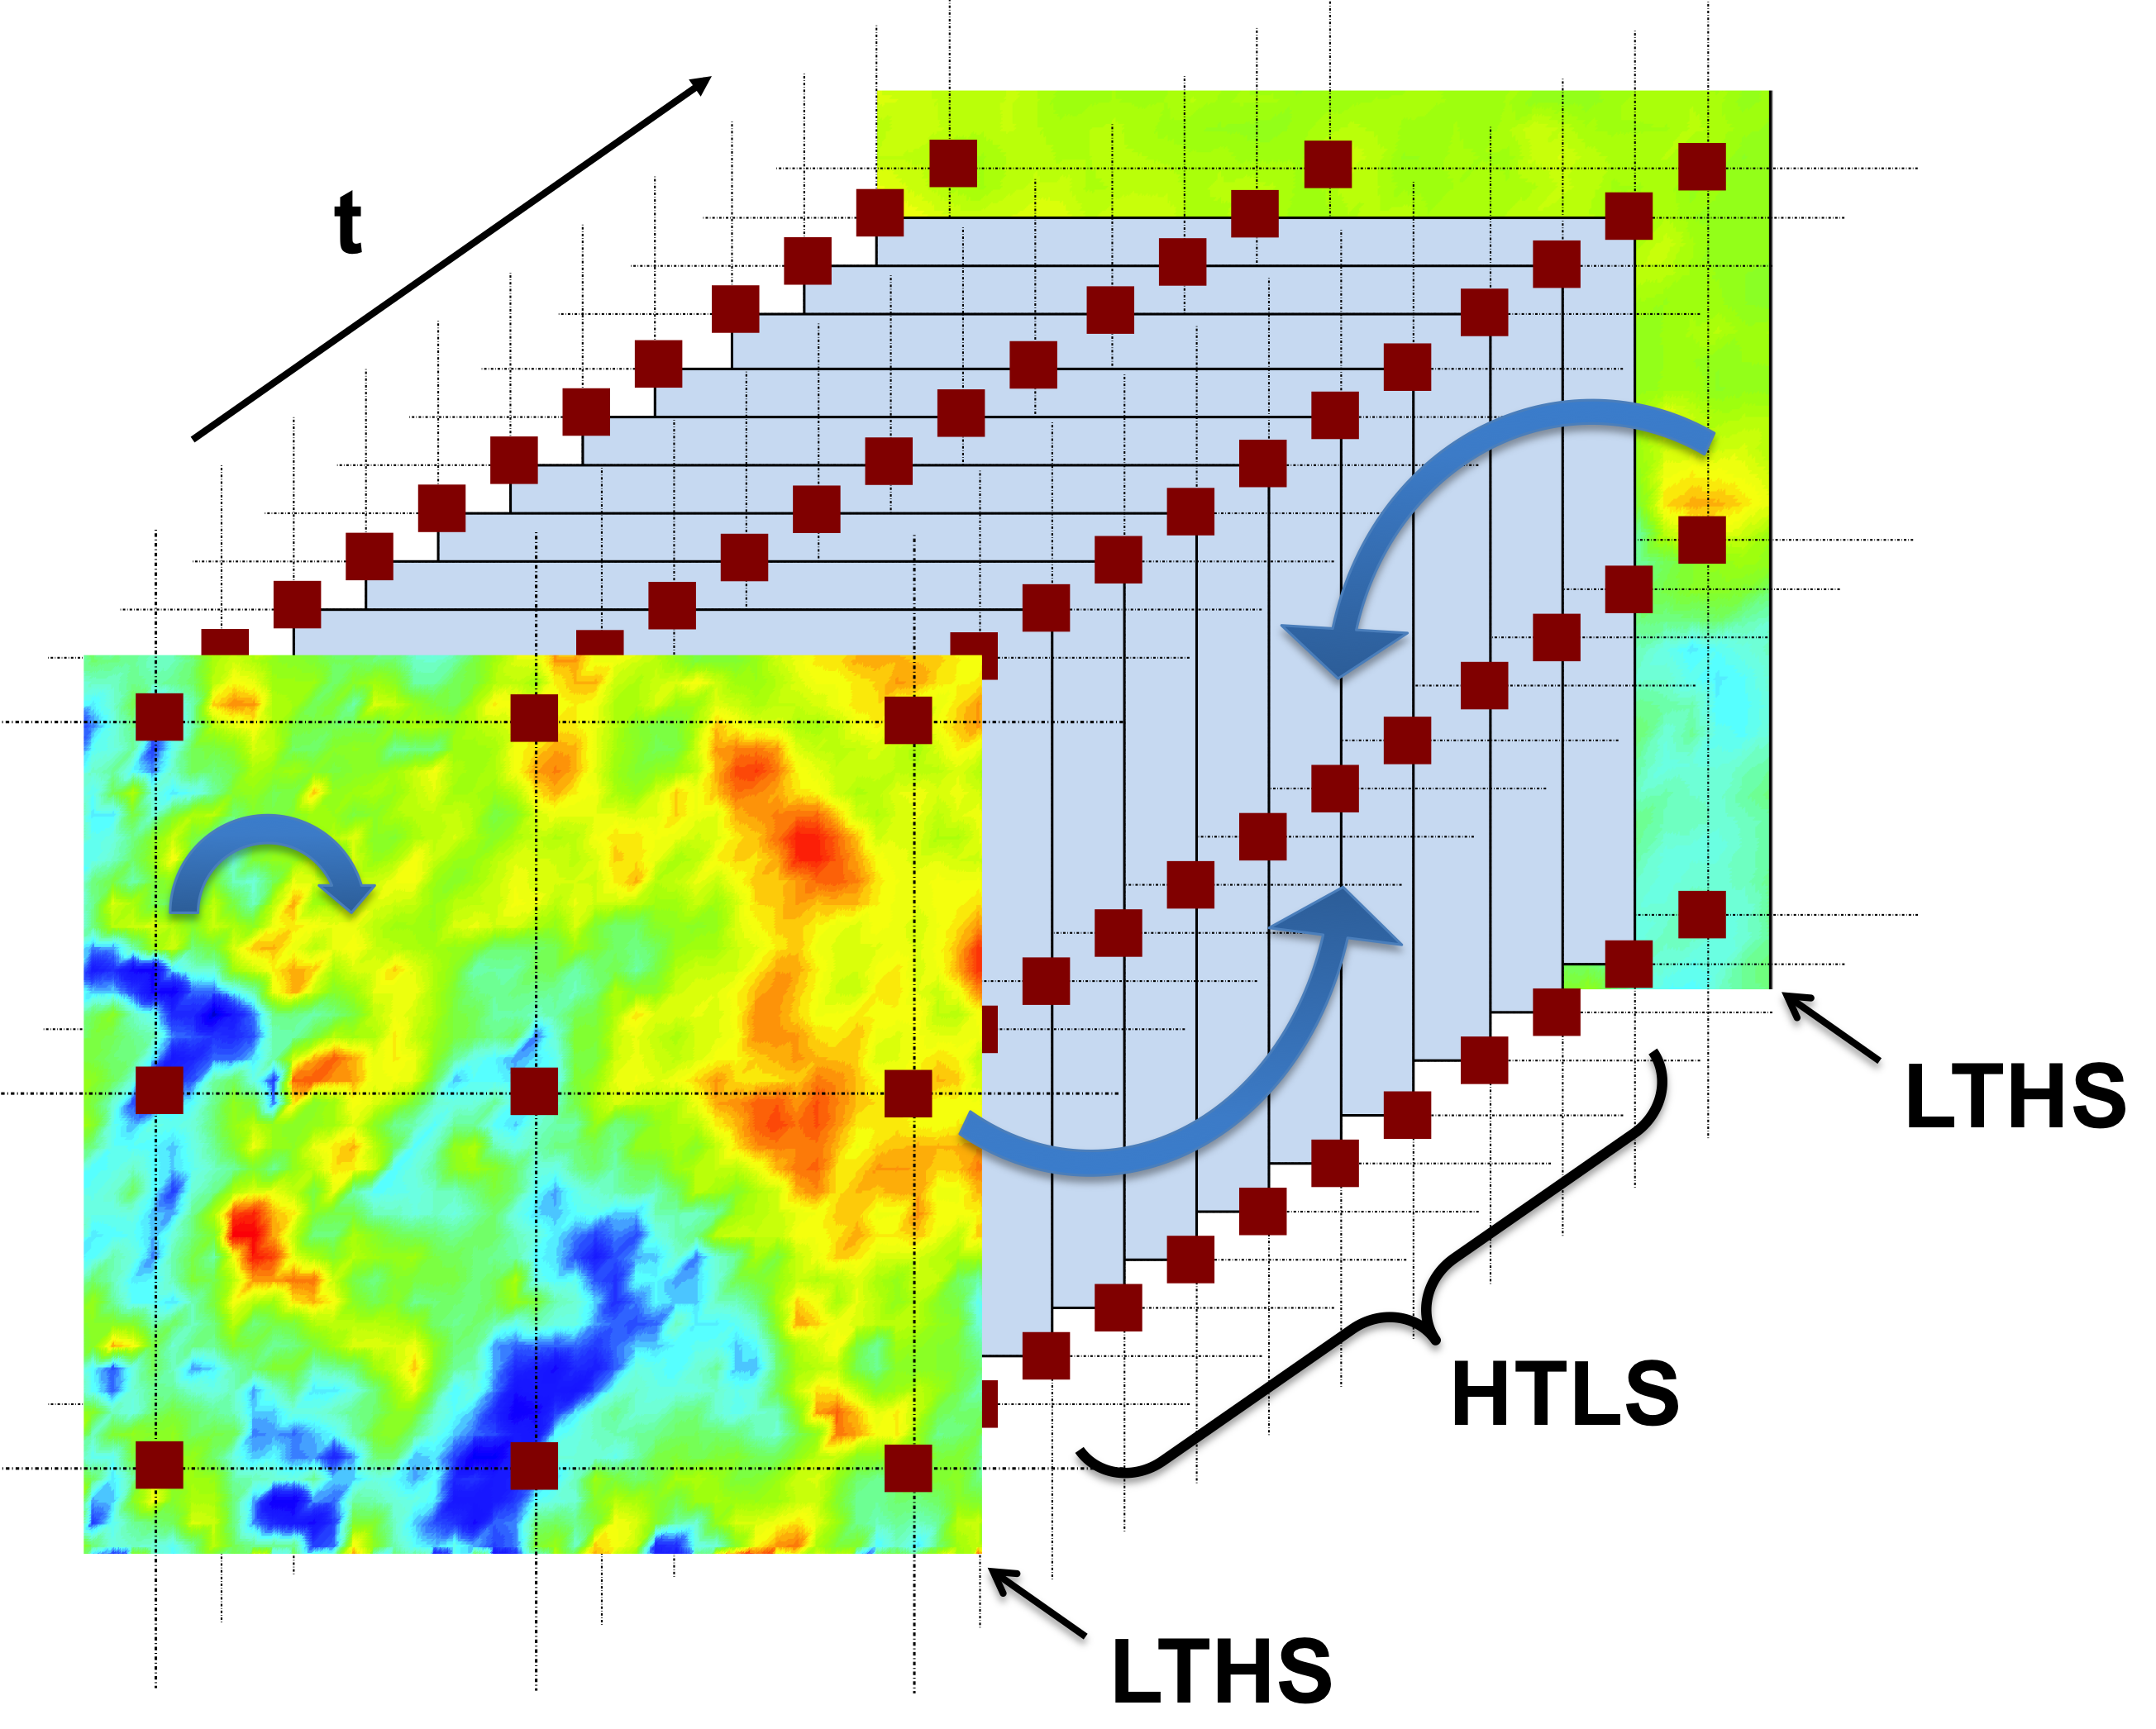
\includegraphics[width=\columnwidth]{./figures/experimentalsetup/experiment_setup_fusion.png}
			\end{figure}
		\end{minipage}
	\end{minipage}
\end{frame}


% % % % % % % % % % % % % % % % % % % % % % % % % % % % % % % % % % % % % % % % % % % % % %
% % % % % % % % % % % % % % % % % % % % % % % % % % % % % % % % % % % % % % % % % % % % % %
% % % % % % % % % % % % % % % % % % % % % % % % % % % % % % % % % % % % % % % % % % % % % % 
\section[Models performances]{Analyses of models performances}
\begin{frame}
\frametitle{Models performances: loss of energy and NRMSE}
	*$ \z $, $ \hat{\z} $ and $ \LPF \z $ are reference, reconstructed and filtered fields

	\begin{minipage}{\textwidth}
		\begin{minipage}{0.5\textwidth}
			\begin{itemize}
			\item Loss of energy:
			\begin{equation*}
				\Delta\kappa=\frac{\sum\limits_{j\in \varmathbb{J}} \z _j^2-\sum\limits_{j\in \varmathbb{J}}{[\LPF\z ]_j^2}}{\displaystyle \sum\limits_{j\in \varmathbb{J}}\z _j^2}
			\end{equation*} 
			\end{itemize}
		\end{minipage}		
		\begin{minipage}{0.5\textwidth}
			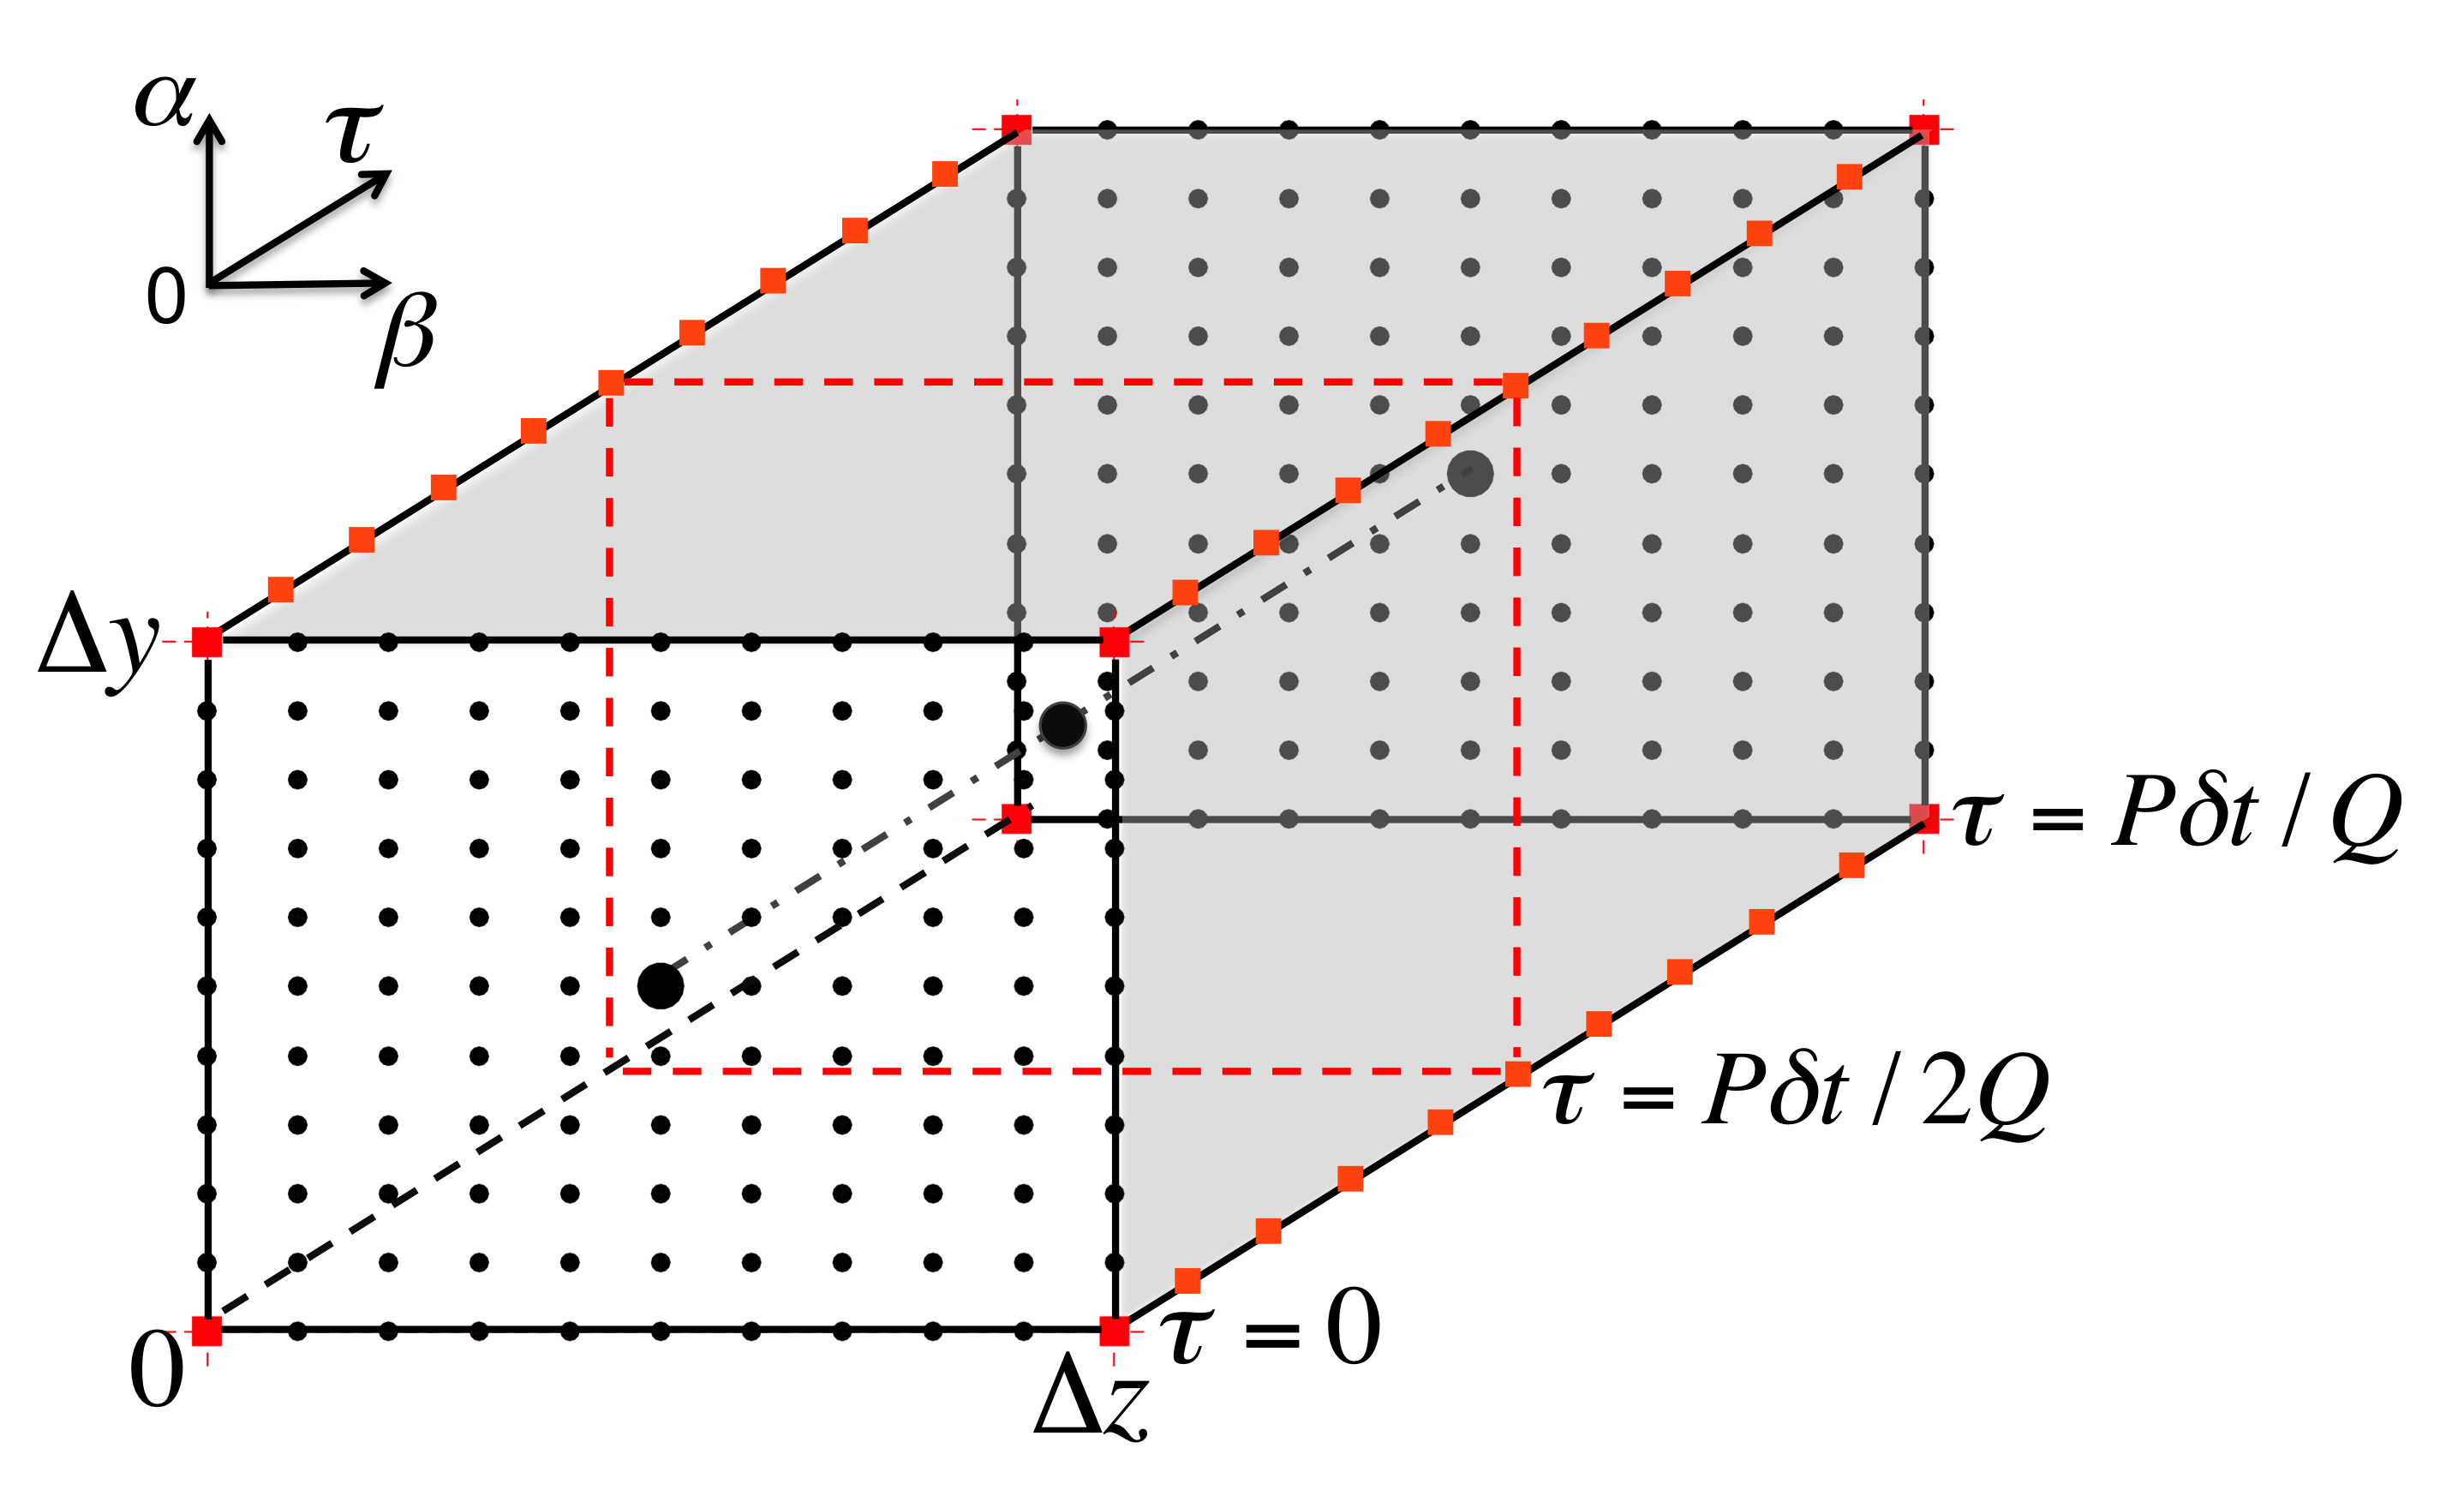
\includegraphics[width=\columnwidth]{./figures/experimentalsetup/elementblock.png}
		\end{minipage}		
	\end{minipage}
	\begin{itemize}	
		\item Normalized Root Mean Squared Error (NRMSE):
		\begin{equation*}
		\epsilon = \left(\frac{ \sum\limits_{t} \sum\limits_{j\in \varmathbb{J}}(\hat{\mybold{z}}_{t,j}-\mybold{z}_{t,j})^2}{\sum\limits_{t} \sum\limits_{j\in \varmathbb{J}}\mybold{z}_{t,j}^2}\right)^{1/2}
		\end{equation*} 
	\end{itemize}		
\end{frame}

\subsection[Isotropic turbulence]{On isotropic turbulence dataset}
\begin{frame}
\frametitle{NRMSEs on isotropic turbulence data}
	\vspace{-0.35cm}
	\begin{figure}
		\hfill \hspace{0cm} 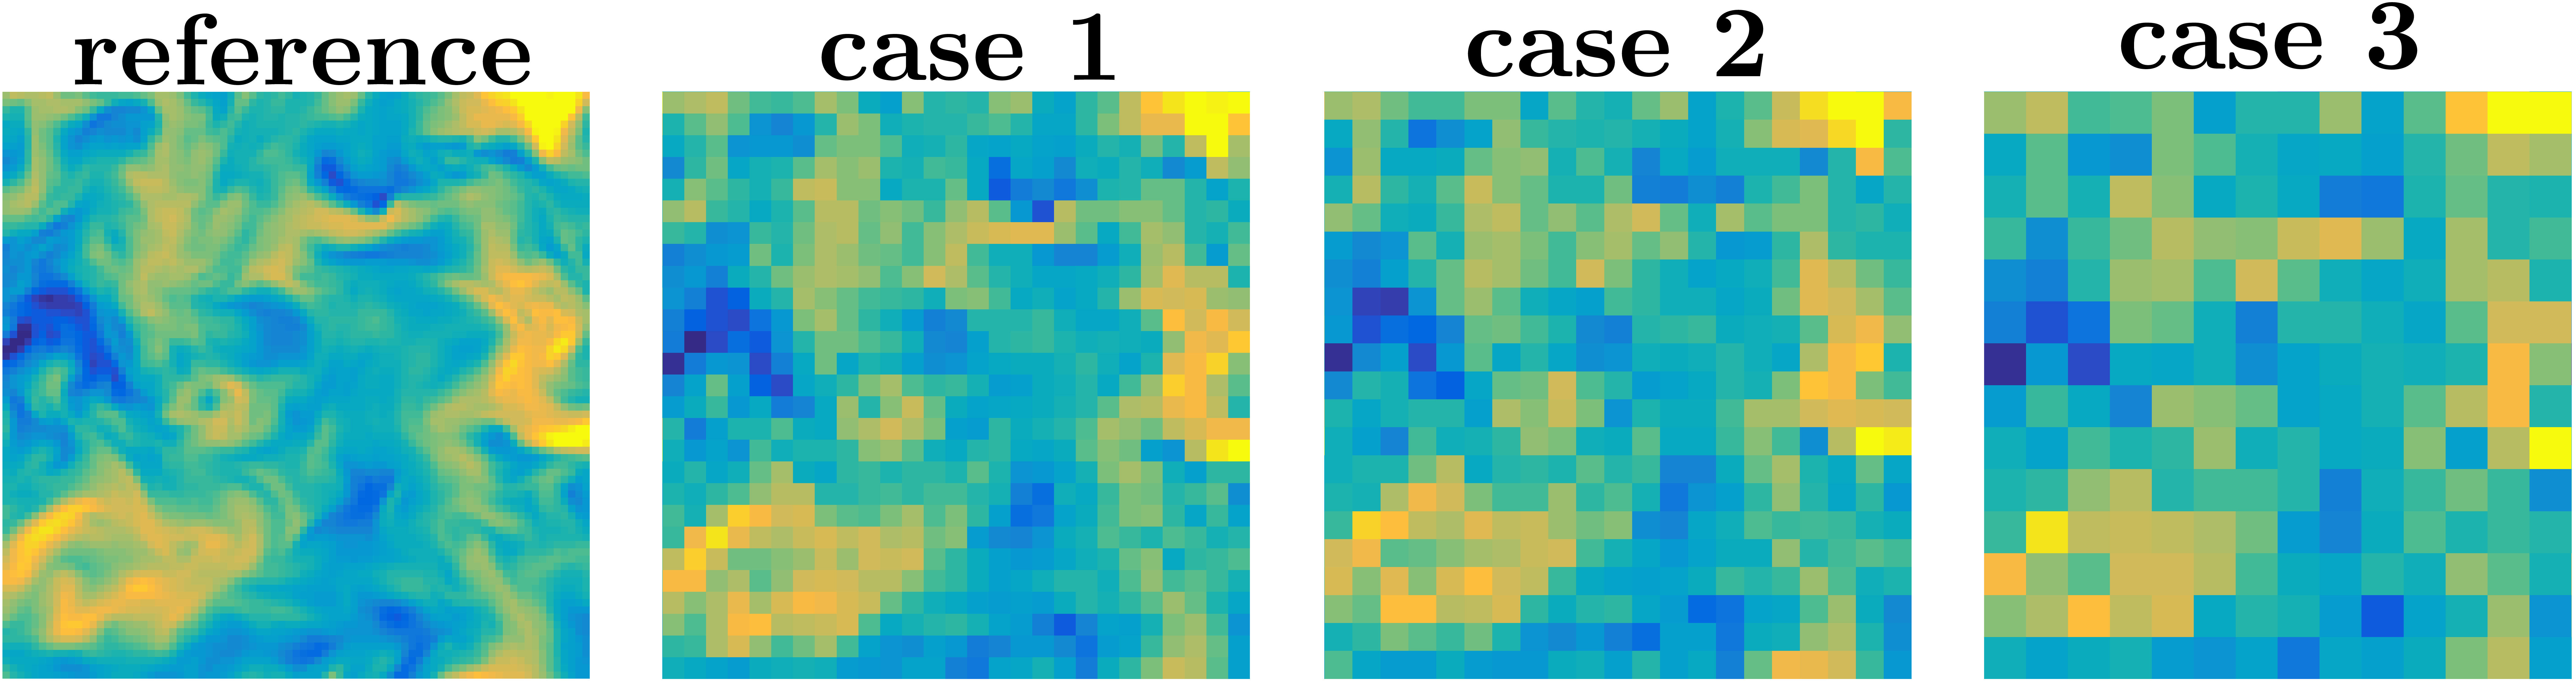
\includegraphics[width=0.5\textwidth]{./figures/turbulence/isotropic/samplesnap_2D_variousratios.png}
	\end{figure}
	\vspace{-0.7cm}
	\begin{overprint}
		\onslide<1>
		\begin{table}
		\centering
			\begin{footnotesize}
			\begin{tabular}{rcccccccc} 
				\toprule 
				&&\multicolumn{3}{c}{$\overline{\epsilon}$}&\multicolumn{1}{c}{}&\multicolumn{3}{c}{$\epsilon_{max}$}\\
				\cmidrule{3-5} \cmidrule{7-9}
				&& {Case 1} & {Case 2} & {Case 3} & & {Case 1} & {Case 2} & {Case 3}\\
				{Method}& {\thead{$(\frac{\dimsh}{\dimsl},\frac{\dimth}{\dimtl})$ \\ $\Delta \kappa$}} & {\thead{($ 3^2,4 $) \\ $ 1 \%$}} & {\thead{($ 4^2,6 $) \\ $ 3 \%$}} & {\thead{($ 6^2,8 $) \\ $ 7 \%$}} & & {\thead{($ 3^2,4 $) \\ $ 1 \%$}} & {\thead{($ 4^2,6 $) \\ $ 3 \%$}} & {\thead{($ 6^2,8 $) \\ $ 7 \%$}}\\
				\midrule 
				\myrowcolour
				$ \Interp_s \y $ && 0.19 & 0.28 & 0.43 & & 0.22 & 0.35 &  0.52 \\ 
				\myrowcolour
				$ \Interp_t \x $ && 0.13 & 0.23 & 0.31 & & 0.19 & 0.28 &  0.42 \\ 	\midrule 
				RR && 0.14 & 0.23 & 0.35 & & 0.20 & 0.34 &  0.50 \\
				KRR && 0.13 & 0.23 & 0.34 & & 0.20 & 0.34 &  0.49 \\ 	\midrule 
				Greedy propag && 0.11 & 0.20 & 0.32 & & 0.18 & 0.33 &  0.51 \\
				Non-greedy propag && 0.11 & 0.19 & 0.30 & & 0.17 & 0.31 &  0.46 \\	
				Fusion (LG)  && 0.11 & 0.18 & 0.27 & & 0.17 &  0.26 &  0.41 \\
		    	Fusion (BF)  && 0.11 & 0.18 & 0.26 & & 0.17 &  0.26 &  0.40 \\ \bottomrule
			\end{tabular}
			\end{footnotesize}
		\end{table}


		\onslide<2>
		\begin{table}
		\centering
			\begin{footnotesize}
			\begin{tabular}{rcccccccc} 
				\toprule 
				&&\multicolumn{3}{c}{$\overline{\epsilon}$}&\multicolumn{1}{c}{}&\multicolumn{3}{c}{$\epsilon_{max}$}\\
				\cmidrule{3-5} \cmidrule{7-9}
				&& {Case 1} & {Case 2} & {Case 3} & & {Case 1} & {Case 2} & {Case 3}\\
				{Method}& {\thead{$(\frac{\dimsh}{\dimsl},\frac{\dimth}{\dimtl})$ \\ $\Delta \kappa$}} & {\thead{($ 3^2,4 $) \\ $ 1 \%$}} & {\thead{($ 4^2,6 $) \\ $ 3 \%$}} & {\thead{($ 6^2,8 $) \\ $ 7 \%$}} & & {\thead{($ 3^2,4 $) \\ $ 1 \%$}} & {\thead{($ 4^2,6 $) \\ $ 3 \%$}} & {\thead{($ 6^2,8 $) \\ $ 7 \%$}}\\
				\midrule 
				$ \Interp_s \y $ && 0.19 & 0.28 & 0.43 & & 0.22 & 0.35 &  0.52 \\ 
				$ \Interp_t \x $ && 0.13 & 0.23 & 0.31 & & 0.19 & 0.28 &  0.42 \\ 	\midrule 
				\myrowcolour			
				RR && 0.14 & 0.23 & 0.35 & & 0.20 & 0.34 &  0.50 \\
				\myrowcolour			
				KRR && 0.13 & 0.23 & 0.34 & & 0.20 & 0.34 &  0.49 \\ 	\midrule 
				Greedy propag && 0.11 & 0.20 & 0.32 & & 0.18 & 0.33 &  0.51 \\
				Non-greedy propag && 0.11 & 0.19 & 0.30 & & 0.17 & 0.31 &  0.46 \\	
				Fusion (LG)  && 0.11 & 0.18 & 0.27 & & 0.17 &  0.26 &  0.41 \\
		    	Fusion (BF)  && 0.11 & 0.18 & 0.26 & & 0.17 &  0.26 &  0.40 \\ \bottomrule	
			\end{tabular}
			\end{footnotesize}
		\end{table}
		
				    	
		\onslide<3>
		\begin{table}
		\centering
			\begin{footnotesize}
			\begin{tabular}{rcccccccc} 
				\toprule 
				&&\multicolumn{3}{c}{$\overline{\epsilon}$}&\multicolumn{1}{c}{}&\multicolumn{3}{c}{$\epsilon_{max}$}\\
				\cmidrule{3-5} \cmidrule{7-9}
				&& {Case 1} & {Case 2} & {Case 3} & & {Case 1} & {Case 2} & {Case 3}\\
				{Method}& {\thead{$(\frac{\dimsh}{\dimsl},\frac{\dimth}{\dimtl})$ \\ $\Delta \kappa$}} & {\thead{($ 3^2,4 $) \\ $ 1 \%$}} & {\thead{($ 4^2,6 $) \\ $ 3 \%$}} & {\thead{($ 6^2,8 $) \\ $ 7 \%$}} & & {\thead{($ 3^2,4 $) \\ $ 1 \%$}} & {\thead{($ 4^2,6 $) \\ $ 3 \%$}} & {\thead{($ 6^2,8 $) \\ $ 7 \%$}}\\
				\midrule  
				$ \Interp_s \y $ && 0.19 & 0.28 & 0.43 & & 0.22 & 0.35 &  0.52 \\ 
				$ \Interp_t \x $ && 0.13 & 0.23 & 0.31 & & 0.19 & 0.28 &  0.42 \\ 	\midrule 			
				RR && 0.14 & 0.23 & 0.35 & & 0.20 & 0.34 &  0.50 \\
				KRR && 0.13 & 0.23 & 0.34 & & 0.20 & 0.34 &  0.49 \\ 	\midrule 
				\myrowcolour
				Greedy propag && 0.11 & 0.20 & 0.32 & & 0.18 & 0.33 &  0.51 \\
				\myrowcolour
				Non-greedy propag && 0.11 & 0.19 & 0.30 & & 0.17 & 0.31 &  0.46 \\	
				\myrowcolour
				Fusion (LG)  && 0.11 & 0.18 & 0.27 & & 0.17 &  0.26 &  0.41 \\
				\myrowcolour
		    	Fusion (BF)  && 0.11 & 0.18 & 0.26 & & 0.17 &  0.26 &  0.40 \\ \bottomrule
			\end{tabular}
			\end{footnotesize}
		\end{table}
		
		\onslide<4>
		\begin{table}
		\centering
			\begin{footnotesize}
			\begin{tabular}{rcccccccc} 
				\toprule 
				&&\multicolumn{3}{c}{$\overline{\epsilon}$}&\multicolumn{1}{c}{}&\multicolumn{3}{c}{$\epsilon_{max}$}\\
				\cmidrule{3-5} \cmidrule{7-9}
				&& {Case 1} & {Case 2} & {Case 3} & & {Case 1} & {Case 2} & {Case 3}\\
				{Method}& {\thead{$(\frac{\dimsh}{\dimsl},\frac{\dimth}{\dimtl})$ \\ $\Delta \kappa$}} & {\thead{($ 3^2,4 $) \\ $ 1 \%$}} & {\thead{($ 4^2,6 $) \\ $ 3 \%$}} & {\thead{($ 6^2,8 $) \\ $ 7 \%$}} & & {\thead{($ 3^2,4 $) \\ $ 1 \%$}} & {\thead{($ 4^2,6 $) \\ $ 3 \%$}} & {\thead{($ 6^2,8 $) \\ $ 7 \%$}}\\
				\midrule 
				$ \Interp_s \y $ && 0.19 & 0.28 & 0.43 & & 0.22 & 0.35 &  0.52 \\ 
				$ \Interp_t \x $ && 0.13 & 0.23 & 0.31 & & 0.19 & 0.28 &  0.42 \\ 	\midrule 			
				RR && 0.14 & 0.23 & 0.35 & & 0.20 & 0.34 &  0.50 \\
				KRR && 0.13 & 0.23 & 0.34 & & 0.20 & 0.34 &  0.49 \\ 	\midrule 
				\myrowcolour
				Greedy propag && \textbf{0.11} & 0.20 & 0.32 & & 0.18 & 0.33 &  0.51 \\
				\myrowcolour
				Non-greedy propag && \textbf{0.11} & 0.19 & 0.30 & & \textbf{0.17} & 0.31 &  0.46 \\	
				\myrowcolour
				Fusion (LG)  && \textbf{0.11} & \textbf{0.18} & 0.27 & & \textbf{0.17} &  \textbf{0.26} &  0.41 \\
				\myrowcolour
		    	Fusion (BF)  && \textbf{0.11} & \textbf{0.18} & \textbf{0.26} & & \textbf{0.17 } &  \textbf{0.26} &  \textbf{0.40} \\ \bottomrule	    		
		\end{tabular}
		\end{footnotesize}
	\end{table}
	\end{overprint}
\end{frame}

\begin{frame}
\frametitle{Spectra of reconstructed fields by various methods}
	\begin{figure}
		\includegraphics[width=\textwidth]{./figures/comparisons/isotropic/spectra_sspacing3_tspacing4_spectra2d_sidelegends.eps}
	\end{figure}
\end{frame}


\subsection[Channel flow]{On turbulent channel flow dataset}

\begin{frame}
\frametitle{NRMSEs on turbulent channel flow data}
	\vspace{-1cm}
	\begin{figure}
		\hfill \includegraphics[width=0.5\textwidth]{./figures/turbulence/channel/samplesnap_2D_variousratios.png}
	\end{figure}
	\vspace{-1.25cm}
	\begin{table}
	\centering
	\begin{small}
		\begin{tabular}{rcccccccc} 
			\toprule 
			&&\multicolumn{3}{c}{$\overline{\epsilon}$}&\multicolumn{1}{c}{}&\multicolumn{3}{c}{$\epsilon_{max}$}\\
			\cmidrule{3-5} \cmidrule{7-9}
			&& {Case 1} & {Case 2} & {Case 3} & & {Case 1} & {Case 2} & {Case 3}\\
			{Method}& {\thead{$(\frac{\dimsh}{\dimsl},\frac{\dimth}{\dimtl})$ \\ $\Delta \kappa$}} & {\thead{($ 5^2,4 $) \\ $ 1 \%$}} & {\thead{($ 10^2,10 $) \\ $ 8 \%$}} & {\thead{($ 20^2,20 $) \\ $ 20 \%$}} & & {\thead{($ 5^2,4 $) \\ $ 1 \%$}} & {\thead{($ 10^2,10 $) \\ $ 8 \%$}} & {\thead{($ 20^2,20 $) \\ $ 20 \%$}}\\ \midrule
			$ \Interp_s \y $ && 0.14 & 0.36 & 0.68 & & 0.16 & 0.47 &  0.85 \\ 
			$ \Interp_t \x $ && 0.11 & 0.32 & 0.54 & & 0.18 & 0.55 &  0.85 \\
			\myrowcolour
			RR && 0.12 & 0.34 & 0.64 & & 0.15 & 0.49 &  0.78 \\
			\myrowcolour
	    	Fusion (BF) && \textbf{0.08} & \textbf{0.25} & \textbf{0.46} & & \textbf{0.13} &  \textbf{0.43} &  \textbf{0.73} \\ 
			\bottomrule
		\end{tabular}
	\end{small}
	\end{table}
	\vspace{-0.2cm}
	\hfill \scriptsize *Errors are estimated in the middle of the channel, $ y/H = [0.5,1.5] $
\end{frame}

\begin{frame}
\frametitle{NRMSEs as functions of position in space}
	\begin{figure}
		\includegraphics[width=0.725\textwidth]{./figures/comparisons/channel/error_MAP_newOM1_boxin4HWs_outer.png}\
		\caption*{NRMSEs averaged over all points at $ y/H=[0.5,1.5] $ and $ (\alpha,\beta) = (\Delta \alpha/2,\Delta \beta/2) $}		
	\end{figure}
\end{frame}

\begin{frame}
\frametitle{NRMSEs as functions of position in time}
	\begin{figure}
		\includegraphics[width=0.8\textwidth]{./figures/comparisons/channel/error_MAP_newOM1_middlepoint_outer.eps}
		\caption*{NRMSEs averaged over all blocks bounded by 4 HTLS measurements at $ y/H=[0.5,1.5] $ and $ \tau = \dimth/2\dimtl $}
	\end{figure}
\end{frame}

\begin{frame}
\frametitle{A sample velocity field}
	\begin{overprint}
		\onslide<1>
			\begin{figure}
				\includegraphics[width=\textwidth]{./figures/comparisons/channel/improper_outer_spacespacing_10_timespacing_10_subplots_t002.png}
				\caption*{A snapshot of reconstructed and reference streamwise velocity field at $ \tau = 2 $}
			\end{figure}
		\onslide<2>
			\begin{figure}
				\includegraphics[width=\textwidth]{./figures/comparisons/channel/improper_outer_spacespacing_10_timespacing_10_subplots_t006.png}
				\caption*{A snapshot of reconstructed and reference streamwise velocity field at $ \tau = \dimth/2\dimtl  = 6$}
			\end{figure}				
	\end{overprint}
\end{frame}

\begin{frame}
\frametitle{A sample time evolution}
	\begin{figure}
		\includegraphics[width=\textwidth]{./figures/comparisons/channel/improper_point_spacespacing_10_timespacing_10_yid129_zid149.eps}
		\caption*{A time evolution of reconstructed and reference streamwise velocity at the center of the channel, $ y/H=1 $ and $ (\alpha,\beta) = (\Delta \alpha/2,\Delta \beta/2)$}
	\end{figure}
\end{frame}



% % % % % % % % % % % % % % % % % % % % % % % % % % % % % % % % % % % % % % % % % % % % % %
% % % % % % % % % % % % % % % % % % % % % % % % % % % % % % % % % % % % % % % % % % % % % %
% % % % % % % % % % % % % % % % % % % % % % % % % % % % % % % % % % % % % % % % % % % % % % 
\section{Conclusions and perspectives}
\subsection[Conclusions]{Conclusions}
\begin{frame}
\frametitle{Conclusions}
\begin{itemize}
	\item Adaptive single models over-perform single interpolation methods
	\item Benefits are observed by combining complementary information
	\item Problems of sampling and aliasing should be considered in future sensing systems
	\item Problems in turbulence are essentially different from image processing
	\item Turbulence is hard, but complex learning algorithms are promising
	\item Learning is powerful, but physics is also crucial
\end{itemize}	
\end{frame}

\subsection[Perspectives]{Suggestions for future works}
\begin{frame}
\frametitle{Suggestions for future works}
\begin{enumerate}[(i)]
	\item \textbf{On the models}
	\begin{itemize}
		\item Using physical prior: Navier-Stokes, divergence-free, turbulence spectra
		\item Highly nonlinear mapping functions with deep neural network, potentially combined with sparse prior
		\item Ensemble of models: further exploit the advantages of all models
		\item Combine fusion and dictionary learning: ADMM 
		\begin{equation*}
			\z = \dict \dictco \:\:\:\: s.t. \:\:\:\: \{\dict,\dictco\} = \argmin_{\dict,\dictco} \left\lbrace \frac{1}{2} \Vert \Sub_t\dict \dictco -\x \Vert^2_{\Sigma_{\h_t}} + \frac{1}{2} \Vert \Sub_s\dict\dictco -\y \Vert^2_{\Sigma_{\h_s}} + \lambda \Vert \dictco \Vert_1 \right\rbrace
		\end{equation*}
	\end{itemize}
\end{enumerate}	
\end{frame}

\begin{frame}
\frametitle{Suggestions for future works}
\begin{enumerate}[(i)]
	\setcounter{enumi}{1}
	\item \textbf{Co-conception design}
	\begin{itemize}
		\item Reconstruction of three-component velocity fields and cross-component quantities (cross-correlation, vorticity)
		\item Handle aliasing
		\item Increase the resolution of PIV measurements by different setups
		\item Design new challenging measurements
	\end{itemize}
\end{enumerate}	
\end{frame}

\subsection[Contributions]{Contributions}
\begin{frame}
\frametitle{Main contributions}
	\begin{minipage}{\textwidth}
		\begin{minipage}[t]{0.425\textwidth}
				This work has resulted in:
				
				{\scriptsize Nguyen et al., (2015). ``A Bayesian fusion model for space-time reconstruction of finely resolved velocities in turbulent flows from low resolution
				measurements''. In: \textit{Journal of Statistical Mechanics: Theory and Experiment} 2015.10, P10008.}
				
				%\hfill\begin{minipage}{\dimexpr\textwidth-0.5cm}
				%\footnotesize Nguyen et al., (2015). ``A Bayesian fusion model for space-time recon-
				%struction of finely resolved velocities in turbulent flows from low resolution
				%measurements''. In: \textit{Journal of Statistical Mechanics: Theory and Experi-
				%ment} 2015.10, P10008.
				%\end{minipage}
				
				and has presented at:
				\begin{itemize}\itemsep0em
					\item \scriptsize 15th European Turbulence conference, Delft, Netherlands
					\item \scriptsize GDR Turbulence, Grenoble, France
				\end{itemize}
				
				Codes are available at:
				
				{\tiny \url{https://github.com/linhvannguyen/}}
				
		\end{minipage}
		\hfill
		\begin{minipage}[t]{0.55\textwidth}
		\begin{figure}[t]
			\vspace*{-0.3cm}
			\includegraphics[width=\columnwidth]{./figures/github.png}
		\end{figure}
		\end{minipage}
	\end{minipage}
\end{frame}


\appendix
\backupbegin
\section{Appendices}
\subsection{References}
\begin{frame}[allowframebreaks]
\frametitle{References}
	\begin{footnotesize}
	\beamertemplatebookbibitems
	\bibliographystyle{apalike}
	\bibliography{bibliographie.bib}
	\end{footnotesize}
\end{frame}

\subsection{Regression}
\begin{frame}
\frametitle{Regression}		
	\begin{tcolorbox}[colback=red!5!white,colframe=red!75!black]	
		\textbf{Parameter estimation} (regularization parameters, size of training data): \emph{bias-variance} trade-off, \textit{k-fold} cross validation 
 	\end{tcolorbox}
 	
	\begin{figure}
	\centering
	\begin{minipage}{.4\textwidth}
	  \includegraphics[height=4.75cm]{./figures/Regression/RR_validationcurve.eps}
	  \caption{Validation curve}
	\end{minipage}
	\hfil
	\begin{minipage}{.4\textwidth}
	  \includegraphics[height=4.75cm]{./figures/Regression/RR_learningcurve.eps}
	  \caption{Learning curve}	
	\end{minipage}
	\end{figure}
\end{frame}	

\subsection{Dictionary learning}
\begin{frame}
	\frametitle{Dictionary learning: error vs sparsity} 
	\begin{figure}
	\centering
		\includegraphics[width=0.95\textwidth]{./figures/DL/Sparsity_vs_NRMSE_PCA_ODL_KSVD_WL_Dau_patchsize04.eps}
		\caption{Sparsity vs error outside the training data}
	\end{figure}
\end{frame}

\subsection{Bayesian fusion}
\begin{frame}
	\frametitle{MAP} 
	\begin{figure}
	\centering
		\includegraphics[width=0.6\textwidth]{./figures/Bayes/MAP.png}
		\caption{Sparsity vs error outside the training data}
	\end{figure}
\end{frame}


\subsection{Results}
\begin{frame}
	\frametitle{Pdfs of velocity increments} 
	\begin{figure}
	\centering
		\includegraphics[height=4.5cm]{./figures/comparisons/channel/pdf_org.pdf}
		\hfill
		\includegraphics[height=4.5cm]{./figures/comparisons/channel/pdf_fusion.pdf}
		\caption{Probability density functions of velocity increments: reference and fusion}
	\end{figure}
\end{frame}

\begin{frame}
	\frametitle{Error map} 
	\begin{figure}
	\centering
		\includegraphics[height=5cm]{./figures/DNSdataset/fusion/errorsmap_average_allscales.png}
		\caption{A map of errors as functions of energy losses}
	\end{figure}
\end{frame}


\begin{frame}
	\frametitle{NLM propagation} 
	\begin{figure}
	\centering
		\includegraphics[height=6.5cm]{./figures/NLM/interpdiff/NLmean_interps_NRMSE_vary_spacespacing.eps}
		\caption{NRMSE when varying the sampling ratio in space}
	\end{figure}
\end{frame}


\begin{frame}
	\frametitle{NLM propagation} 
	\begin{figure}
	\centering
		\includegraphics[height=6.5cm]{./figures/NLM/interpdiff/NLmean_interps_NRMSE_vary_timespacing.eps}
		\caption{NRMSE when varying the sampling ratio in time}
	\end{figure}
\end{frame}
\backupend


\end{document} 